% !TEX program = pdflatex
% !TeX encoding = utf8
% !TeX spellcheck = pl-PL

%%%%%%%%%%%%%%%%%%%%%%%%%%%%%%%%%%%%%%%%%%%%%%%%%%%%%%%%%%%%%%%%%%%%%%%%%%%
% Wybierz rodzaj pracy dyplomowej oraz wydział
% Pick thesis type and faculty
%%%%%%%%%%%%%%%%%%%%%%%%%%%%%%%%%%%%%%%%%%%%%%%%%%%%%%%%%%%%%%%%%%%%%%%%%%%
\documentclass[thesis=mgr,faculty=ee]{EE-dyplom} 

% thesis=[inz|mgr|bsc|msc]
%  * inz - praca inżynierska
%  * mgr - praca magisterska
%  * bsc - bachelor thesis
%  * msc - master thesis

% Skróty nazw wydziałów zgodne z domenami internetowymi
% Abbreviations of Faculties according to Internet subdomains
% faculty=[
%	arch,
%	gik,
%	ee,
%	wip
%	]

%%%%%%%%%%%%%%%%%%%%%%%%%%%%%%%%%%%%%%%%%%%%%%%%%%%%%%%%%%%%%%%%%%%%%%%%%%%
% Konfiguracja - do personalizacji
% Configuration - to be personalized
%%%%%%%%%%%%%%%%%%%%%%%%%%%%%%%%%%%%%%%%%%%%%%%%%%%%%%%%%%%%%%%%%%%%%%%%%%%
\instytut{Instytut Elektrotechniki Teoretycznej i Systemów Informacyjno-Pomiarowych}
\kierunek{Elektrotechnika}
\specjalnosc{Systemy wbudowane}
\title{Badanie właściwości statystycznych generatora bitów losowych zaimplementowanego w układzie FPGA}
\engtitle{Study of the statistical properties of a random bit generator implemented in an FPGA system}
\album{318887}
\author{inż. Gerard Boruszewicz}
\promotor{dr inż. Łukasz Makowski}
\date{2026}
\longdate{2077-07-27}

%%%%%%%%%%%%%%%%%%%%%%%%%%%%%%%%%%%%%%%%%%%%%%%%%%%%%%%%%%%%%%%%%%%%%%%%%%%
% Streszczenie pracy i abstract.
% In case of thesis in English swap the order - English version goes first.
%%%%%%%%%%%%%%%%%%%%%%%%%%%%%%%%%%%%%%%%%%%%%%%%%%%%%%%%%%%%%%%%%%%%%%%%%%%
\streszczeniepracy{

W pracy przedstawiono projekt, implementację oraz analizę statystyczną generatora bitów
losowych opartego na oscylatorach pierścieniowych, zrealizowanego w układzie
programowalnym FPGA Xilinx Spartan-7 na płytce rozwojowej Arty S7-25. Źródłem entropii
jest jitter przebiegów generowanych przez łańcuchy inwerterów o zróżnicowanej długości,
zamknięte w pętle sprzężenia zwrotnego. Bity pozyskiwane są metodą detekcji zboczy
w próbkowanych przebiegach, gromadzone w buforze i przekazywane do komputera interfejsem
UART z zastosowaniem mechanizmu potwierdzania gotowości.

Zasadniczą część pracy stanowi analiza wpływu decyzji projektowych na właściwości
statystyczne uzyskiwanego strumienia. Zbadano cztery konfiguracje generatora, różniące
się liczbą oscylatorów, sposobem ich rozmieszczenia w strukturze układu, obecnością
operacji różnicy symetrycznej na wyjściach oraz zastosowaniem korekcji rozkładu metodą
von  Neumanna. Dla każdej z nich zarejestrowano serię o długości $10\,485\,760$ bitów
i poddano ją trzem niezależnym badaniom: analizie odchylenia rozkładu z wykorzystaniem
testu monobitowego, analizie autokorelacji oraz analizie dwuwymiarowych map rozkładu słów
wielobitowych. Narzędzia do akwizycji i analizy danych opracowano w języku Python.

Wyniki wykazały, że zastosowane metody prowadzą do odmiennego uszeregowania badanych
konfiguracji. Ręczne rozproszenie oscylatorów w strukturze układu zredukowało odchylenie
rozkładu z  jedenastu do jednego odchylenia standardowego, jednocześnie pogarszając wynik
autokorelacji o blisko dwa rzędy wielkości. Zwiększenie liczby oscylatorów wraz
z łączeniem ich wyjść operacją różnicy symetrycznej ograniczyło amplitudę zależności
czasowych blisko dwudziestoośmiokrotnie, natomiast korekcja metodą von Neumanna usunęła
uporządkowaną strukturę współczynników autokorelacji oraz nierównomierność rozkładu
wartości słów. Analiza wskazała warstwę serializacji strumienia jako mechanizm
odpowiedzialny za zasadniczą część wykrytych odstępstw od losowości oraz wykazała, że
ocena źródła entropii oparta na jednej metryce statystycznej jest niewystarczająca. 

} % koniec streszczenia

\slowakluczowe{generator liczb losowych, TRNG, oscylator pierścieniowy, FPGA,
VHDL, jitter, entropia, analiza statystyczna, korekcja von  Neumanna, UART}

\thesisabstract{

This thesis presents the design, implementation and statistical analysis of a random bit
generator based on ring oscillators, implemented in a Xilinx Spartan-7 field-programmable
gate array on an Arty S7-25 development board. The entropy source is the jitter of
waveforms produced by inverter chains of varying length closed in feedback loops. Bits are
extracted by detecting edges in the sampled waveforms, accumulated in a buffer and
transmitted to a host computer over a UART interface using a ready-valid handshake
mechanism.

The core of the work is an analysis of how design decisions affect the statistical
properties of the resulting bitstream. Four generator configurations were examined,
differing in the number of oscillators, their placement within the device fabric, the
presence of an exclusive-or operation combining their outputs, and the application of
von Neumann distribution correction. For each configuration a series of $10\,485\,760$
bits was recorded and subjected to three independent tests: distribution bias analysis
using the monobit test, autocorrelation analysis, and analysis of two-dimensional delay
maps of multi-bit words. The acquisition and analysis tools were developed in Python.

The results show that the applied methods rank the configurations differently. Manual
distribution of the oscillators across the device fabric reduced the distribution bias
from eleven to one standard deviation while degrading the autocorrelation result by
almost two orders of magnitude. Doubling the number of oscillators and combining their
outputs with an exclusive-or operation reduced the amplitude of temporal dependencies
by a factor of nearly twenty-eight, whereas von Neumann correction removed both the
ordered structure of the autocorrelation coefficients and the non-uniformity in the
distribution of word values. The analysis identified the bitstream serialisation layer
as the mechanism responsible for the majority of the detected departures from randomness,
and demonstrated that assessing an entropy source on the basis of a single statistical
metric is insufficient.

} % end of abstract

\thesiskeywords{random number generator, TRNG, ring oscillator, FPGA, VHDL, jitter,
entropy, statistical analysis, von Neumann correction, UART}

%%%%%%%%%%%%%%%%%%%%%%%%%%%%%%%%%%%%%%%%%%%%%%%%%%%%%%%%%%%%%%%%%%%%%%%%%%%
% Tu zaczyna się dokument
% Here is the beginning of the document
%%%%%%%%%%%%%%%%%%%%%%%%%%%%%%%%%%%%%%%%%%%%%%%%%%%%%%%%%%%%%%%%%%%%%%%%%%%
\begin{document}
    % Strony nagłówkowe - musi być
    % Headers - must exist
    \frontpages
    
    % Tekst pracy - osobne pliki do edycji
    % Thesis text - separate files for edition

	\chapter{Wstęp}

Liczby losowe stanowią fundament współczesnych systemów bezpieczeństwa informacji.
Wykorzystywane są do generowania kluczy kryptograficznych, wektorów inicjujących,
identyfikatorów sesji oraz wartości jednorazowych, a także w metodach symulacyjnych
Monte Carlo i w algorytmach randomizowanych. W zastosowaniach kryptograficznych jakość
źródła losowości decyduje o bezpieczeństwie całego systemu: nawet poprawnie
zaimplementowany algorytm szyfrowania nie zapewnia ochrony, jeżeli klucz został
wygenerowany w sposób przewidywalny. Historia kryptografii praktycznej dostarcza wielu
przykładów podatności, których źródłem był nie sam algorytm, lecz wadliwy generator
liczb losowych.

Powszechnie stosowane generatory pseudolosowe, oparte na deterministycznych algorytmach,
wytwarzają ciągi o bardzo dobrych właściwościach statystycznych, jednak ich stan
wewnętrzny jest w pełni określony przez wartość początkową. Ciąg taki jest zatem
odtwarzalny, a jego nieprzewidywalność ma charakter wyłącznie obliczeniowy. Tam, gdzie
wymagana jest losowość o charakterze fizycznym, konieczne jest sięgnięcie do zjawisk
niedeterministycznych zachodzących w sprzęcie. Jednym z najczęściej wykorzystywanych
w układach cyfrowych źródeł tego rodzaju jest jitter, czyli losowa fluktuacja momentów
przejść sygnału zegarowego, wynikająca z szumu termicznego i migotania w elementach
półprzewodnikowych.

Układy programowalne FPGA są dla implementacji generatorów sprzętowych platformą
szczególnie atrakcyjną. Umożliwiają realizację źródła entropii wyłącznie przy użyciu
dostępnych zasobów logicznych, bez konieczności stosowania dedykowanych elementów
analogowych, a jednocześnie pozwalają na swobodną modyfikację architektury oraz na pełną
kontrolę nad rozmieszczeniem struktur w obrębie układu. Najczęściej stosowanym
rozwiązaniem tej klasy jest oscylator pierścieniowy, złożony z zamkniętego w pętlę
łańcucha inwerterów o nieparzystej długości, którego przebieg wyjściowy podlega
kumulującemu się jitterowi. Prostota tej struktury jest jednak pozorna: uzyskana jakość
strumienia bitów zależy nie tylko od samego opisu logiki, lecz również od sposobu
odwzorowania jej w zasobach układu, wzajemnego położenia oscylatorów oraz przyjętego
mechanizmu ekstrakcji bitów z próbkowanego przebiegu.

Celem niniejszej pracy jest zaprojektowanie, implementacja oraz przeprowadzenie analizy
statystycznej generatora bitów losowych opartego na oscylatorach pierścieniowych
w strukturze układu FPGA. Praca nie ogranicza się do wykazania działania pojedynczej
implementacji: zasadniczym jej przedmiotem jest zbadanie, w jaki sposób wybrane decyzje
projektowe wpływają na właściwości statystyczne uzyskiwanego strumienia. Analizie poddano
cztery konfiguracje generatora, różniące się liczbą oscylatorów, sposobem ich
rozmieszczenia w strukturze układu, obecnością operacji różnicy symetrycznej na wyjściach
oraz zastosowaniem korekcji rozkładu metodą von Neumanna. Każdą z nich zbadano trzema
niezależnymi metodami: analizą odchylenia rozkładu bitów, badaniem autokorelacji oraz
analizą dwuwymiarowych map rozkładu słów wielobitowych.

Praca składa się z sześciu rozdziałów. Rozdział drugi przedstawia podstawy teoretyczne
analizy statystycznej ciągów losowych: miary entropii, pojęcie ciągu losowego, aparat
testowania hipotez oraz zastosowane w dalszej części metody badawcze wraz z omówieniem
kondycjonowania strumienia i standaryzowanych pakietów testów. Rozdział trzeci omawia
generatory liczb losowych w technice cyfrowej, ich klasyfikację i model funkcjonalny,
a następnie oscylator pierścieniowy jako źródło entropii, ze szczególnym uwzględnieniem
stochastycznego modelu jitteru oraz zjawisk ograniczających entropię. Rozdział czwarty
opisuje wykonaną implementację: wybór platformy sprzętowej, realizację poszczególnych
modułów w języku VHDL oraz interfejs komunikacyjny służący do transmisji danych do
komputera. Rozdział piąty, stanowiący zasadniczą część badawczą, przedstawia narzędzia
programowe opracowane do akwizycji i analizy danych, parametry badanych konfiguracji
oraz wyniki wszystkich przeprowadzonych badań, wraz z ich interpretacją. Rozdział szósty
zawiera podsumowanie pracy oraz wskazanie kierunków dalszego rozwoju.
    \chapter{Metody analizy statystycznej strumienia bitów losowych}

Rozdział łączy omówienie miar entropii, pojęcia losowości oraz metod analizy
statystycznej. Połączenie to jest celowe: entropii nie da się omówić bez
wskazania konkretnej miary, a każda praktycznie stosowana miara entropii jest
estymowana z ciągu bitów procedurami statystycznymi. Metody analizy
statystycznej nie są zatem oddzielnym zagadnieniem, lecz aparatem pomiarowym
entropii.

\section{Miary entropii}

Niech $X$ będzie dyskretną zmienną losową o rozkładzie $p_1,\dots,p_n$.
Stosowane w ocenie generatorów miary tworzą rodzinę entropii Rényiego
rzędu $\alpha$ \cite{renyi1961}:
%
\begin{equation}
  H_\alpha(X) = \frac{1}{1-\alpha}\log_2\sum_{i=1}^{n} p_i^{\alpha},
  \qquad \alpha > 0,\ \alpha \neq 1 .
  \label{eq:renyi}
\end{equation}
%
Szczególne przypadki wyrażenia \eqref{eq:renyi} mają w kontekście generatorów
odrębną interpretację:

\begin{itemize}
  \item \textbf{entropia Shannona} ($\alpha \to 1$):
        \begin{equation}
          H_1(X) = -\sum_{i=1}^{n} p_i \log_2 p_i ,
          \label{eq:shannon}
        \end{equation}
        średnia liczba bitów informacji na symbol, miara przyjęta
        w AIS-31 \cite{killmann2011ais31};
  \item \textbf{entropia kolizji} ($\alpha = 2$):
        \begin{equation}
          H_2(X) = -\log_2\sum_{i=1}^{n} p_i^2 ,
          \label{eq:kolizji}
        \end{equation}
        związana z prawdopodobieństwem kolizji, wykorzystywana
        w estymatorach i w twierdzeniach o ekstrakcji losowości;
  \item \textbf{min-entropia} ($\alpha \to \infty$):
        \begin{equation}
          H_\infty(X) = -\log_2 \max_{i} p_i ,
          \label{eq:minentropia}
        \end{equation}
        miara najgorszego przypadku, odpowiadająca prawdopodobieństwu
        odgadnięcia wartości przy jednej próbie, podstawowa miara
        w SP 800-90B \cite{turan2018sp80090b}, normie określającej wymagania stawiane źródłom entropii stosowanym w generatorach bitów losowych oraz procedury ich walidacji.
\end{itemize}

Zachodzi porządek
%
\begin{equation}
  H_\infty(X) \le H_2(X) \le H_1(X) \le \log_2 n ,
  \label{eq:porzadek}
\end{equation}
%
przy czym w zastosowaniach kryptograficznych istotna jest właśnie miara
najsłabsza. Ilustruje to przykład źródła Bernoulliego o obciążeniu $p$,
zestawiony w tabeli \ref{tab:entropia-obciazenie}.

\begin{table}[htbp]
  \centering
  \caption{Entropia Shannona i min-entropia źródła Bernoulliego
           w funkcji obciążenia}
  \label{tab:entropia-obciazenie}
  \begin{tabular}{ccc}
    \hline
    $p = P(X = 1)$ & $H_1$ [bit/bit] & $H_\infty$ [bit/bit] \\
    \hline
    $0{,}50$ & $1{,}000$ & $1{,}000$ \\
    $0{,}55$ & $0{,}993$ & $0{,}862$ \\
    $0{,}60$ & $0{,}971$ & $0{,}737$ \\
    $0{,}70$ & $0{,}881$ & $0{,}515$ \\
    $0{,}80$ & $0{,}722$ & $0{,}322$ \\
    \hline
  \end{tabular}
\end{table}

Dla małego obciążenia $p = \tfrac{1}{2} + \varepsilon$ zachodzą przybliżenia
%
\begin{equation}
  H_1 \approx 1 - \frac{2}{\ln 2}\,\varepsilon^2 ,
  \qquad
  H_\infty \approx 1 - \frac{2}{\ln 2}\,\varepsilon .
  \label{eq:przyblizenia}
\end{equation}
%
Entropia Shannona maleje więc kwadratowo, a min-entropia liniowo. Pierwsza
z miar jest zatem nadmiernie \emph{optymistyczna}: źródło o obciążeniu
$p = 0{,}6$ wygląda w niej niemal idealnie ($0{,}971$), a w kategoriach
odgadywalności traci ponad jedną czwartą siły. Dla klucza 128-bitowego
złożonego z takich bitów efektywna siła wynosi około 94 bity.

\subsection{Entropia źródeł z pamięcią}

W przypadku źródeł z pamięcią rozkład brzegowy nie wystarcza - konieczne
jest posługiwanie się \textbf{entropią warunkową}
$H(X_n \mid X_{n-1},\dots,X_1)$ oraz \textbf{stopą entropii} procesu
stacjonarnego \cite{cover2006elements}:
%
\begin{equation}
  \bar{H} = \lim_{n \to \infty} \frac{1}{n} H(X_1,\dots,X_n),
  \label{eq:stopa-entropii}
\end{equation}
%
a w praktyce modelami Markowa skończonego rzędu. Zaniedbanie zależności
czasowych jest jednym z najczęstszych błędów oceny generatorów sprzętowych:
ciąg o idealnym rozkładzie brzegowym i silnej autokorelacji ma stopę entropii
znacznie mniejszą od jedności.

Znaczenie tego rozróżnienia dla praktyki pomiarowej jest bezpośrednie.
Rozkład brzegowy bada się miarą obciążenia (bias) i testem monobitowym,
natomiast obecność pamięci - funkcją autokorelacji oraz rozkładem słów
wielobitowych. Są to dwie \emph{niezależne} rodziny własności: strumień może
przejść pomiarowo pierwszą z nich i całkowicie zawieść w drugiej. Dlatego
w części doświadczalnej niniejszej pracy oba aspekty analizowane są osobno,
a nie jako pojedyncza ocena jakości strumienia.

\section{Pojęcie ciągu losowego}

Miary wprowadzone powyżej opisują \emph{źródło}. Osobnym pytaniem jest, co
znaczy, że konkretny \emph{ciąg} jest losowy. Historycznie ukształtowały się
trzy podejścia do formalizacji tego pojęcia.

\paragraph{Podejście częstościowe (statystyczne).}
Zapoczątkowane przez Richarda von Misesa \cite{vonmises1919} pojęcie
\emph{Kollektiv} (ang. \emph{collective}) wymaga, aby częstości symboli
w ciągu i we wszystkich jego podciągach wybranych dopuszczalną regułą były
zbieżne do wartości oczekiwanych. Zbiór dopuszczalnych reguł wyboru
doprecyzował Church \cite{church1940}, ograniczając go do reguł obliczalnych.
Jean Ville \cite{ville1939} wykazał, że warunki tego typu nie wystarczają:
istnieją ciągi spełniające je, a jednocześnie wykazujące jawną regularność
(na przykład sumy częściowe zawsze po jednej stronie wartości oczekiwanej).
Podejście to jest natomiast bezpośrednim źródłem konstrukcji testów
statystycznych, ponieważ każdy test bada jedną wybraną własność częstościową.

\paragraph{Podejście złożonościowe.}
Według Kołmogorowa \cite{kolmogorov1965three} i Martina-Löfa
\cite{martinlof1966} ciąg jest losowy, jeśli nie istnieje jego opis krótszy
od samego ciągu, co oznacza, że jego złożoność algorytmiczna jest bliska
jego długości. Złożoność Kołmogorowa jest nieobliczalna, więc nie istnieje
uniwersalny, skończony test losowości. Ma to fundamentalną konsekwencję
praktyczną: badanie generatora może jedynie falsyfikować hipotezę
o losowości, nigdy natomiast jej nie potwierdzi.

\paragraph{Podejście obliczeniowe (nieprzewidywalność).}
W kryptografii przyjmuje się kryterium nieodróżnialności obliczeniowej od
ciągu idealnego \cite{yao1982theory}, które jest równoważne testowi
następnego bitu \cite{blum1984how,goldreich2001foundations}. Generator jest
bezpieczny, jeśli żaden algorytm o ograniczonych zasobach nie przewiduje
kolejnego bitu z prawdopodobieństwem istotnie większym niż $1/2$. Do tego
dochodzą wymagania dotyczące kompromitacji stanu wewnętrznego. Odporność na
cofanie (ang. \emph{backtracking resistance}) oznacza, że ujawnienie stanu
nie pozwala odtworzyć bitów wcześniejszych. Odporność na przewidywanie
(ang. \emph{prediction resistance}) oznacza, że ujawnienie stanu nie pozwala
przewidzieć bitów przyszłych po dostarczeniu do generatora świeżej entropii
\cite{barker2015sp80090a}. Podobne wymagania, nazywane tajnością wprzód
i wstecz (ang. \emph{forward/backward secrecy}), formułuje AIS~20
\cite{killmann2011ais31}.

\subsection{Ograniczenia testów statystycznych a ocena źródła}

Warto na tym tle wskazać ograniczenie testów statystycznych. Rozważmy rejestr
przesuwny ze sprzężeniem liniowym (ang. \emph{Linear Feedback Shift
Register}, LFSR). Jest to układ złożony z $m$ komórek pamięci, w którym
w każdym takcie zawartość rejestru przesuwa się o jedną pozycję, a nowy bit
wprowadzany na jego początek jest sumą modulo~2 (operacją XOR) wybranych
komórek, zwanych odczepami. Generowany ciąg $s_t$ spełnia zależność
rekurencyjną
%
\begin{equation}
  s_{t+m} = \bigoplus_{j=0}^{m-1} c_j\, s_{t+j},
  \qquad c_j \in \{0,1\},
  \label{eq:lfsr}
\end{equation}
%
w której współczynniki $c_j$ wskazują położenie odczepów i wyznaczają
wielomian charakterystyczny $P(x) = x^m + \sum_{j=0}^{m-1} c_j x^j$ nad ciałem
$\mathrm{GF}(2)$. Jeżeli $P(x)$ jest wielomianem pierwotnym, to rejestr
zainicjowany dowolnym stanem niezerowym generuje ciąg o maksymalnym okresie
$2^m - 1$, zwany ciągiem $m$ \cite{golomb1982shift}. Ciąg taki ma własności,
których oczekuje się od ciągu losowego. W jednym okresie liczba jedynek
różni się od liczby zer o jeden, rozkład długości serii jest zgodny
z rozkładem idealnym, a autokorelacja przyjmuje dwie wartości, zbliżone do
zera dla wszystkich przesunięć niezerowych. Ciąg przechodzi więc większość
klasycznych testów statystycznych.

Jednocześnie jest on całkowicie deterministyczny. Cały ciąg wynika
z $m$-bitowego stanu początkowego i znanych odczepów, a algorytm
Berlekampa-Masseya \cite{massey1969shift} odtwarza strukturę rejestru już
na podstawie $2m$ kolejnych bitów wyjścia. Entropia takiego ciągu nie
przekracza $m$ bitów, niezależnie od jego długości, ponieważ każdy bit
wynika z pierwotnego stanu. Na przykład ciąg o długości $10^6$ bitów
wytworzony przez rejestr 32-bitowy zawiera co najwyżej 32 bity entropii,
a entropia przypadająca na bit maleje do zera wraz z długością ciągu.

Wniosek ma znaczenie dla dalszej części pracy. Test statystyczny ocenia
\emph{ciąg}, natomiast entropia jest własnością \emph{mechanizmu}, który
ten ciąg wytwarza. Wynik pozytywny nie dowodzi więc nieprzewidywalności,
a ocena źródła musi opierać się na modelu jego działania i na analizie
surowych próbek przed jakąkolwiek obróbką deterministyczną
\cite{turan2018sp80090b}.

\section{Aparat testowania hipotez}

Każdy test statystyczny losowości ma tę samą strukturę formalną. Formułuje
się hipotezę zerową
%
\begin{equation}
  H_0: \text{badany ciąg jest realizacją źródła i.i.d. o } P(0) = P(1) = \tfrac{1}{2},
  \label{eq:h0}
\end{equation}
%
wyznacza statystykę testową $T$, której rozkład przy prawdziwości $H_0$ jest
znany (najczęściej asymptotycznie normalny lub $\chi^2$), i oblicza się
wartość $p$ jako prawdopodobieństwo uzyskania wyniku co najmniej tak
skrajnego jak zaobserwowany:
%
\begin{equation}
  p = P\big(|T| \ge |t_{\mathrm{obs}}| \;\big|\; H_0\big).
  \label{eq:pvalue}
\end{equation}
%
Hipotezę odrzuca się, gdy $p < \alpha$, gdzie $\alpha$ jest przyjętym
poziomem istotności (w pakiecie SP 800-22 standardowo $\alpha = 0{,}01$).
Interpretacja wyniku wymaga trzech zastrzeżeń, istotnych dla poprawnego
odczytania rezultatów pomiarowych.

Po pierwsze, $p \ge \alpha$ oznacza wyłącznie brak podstaw do odrzucenia
$H_0$, nigdy jej potwierdzenia - co jest bezpośrednią konsekwencją
nieobliczalności złożoności Kołmogorowa omówionej wcześniej.

Po drugie, przy wielokrotnym testowaniu odrzucenia pojawiają się z
częstością $\alpha$ nawet dla źródła idealnego. Dla $k$ niezależnych testów
oczekiwana liczba fałszywych odrzuceń wynosi $k\alpha$, a przy $\alpha = 0{,}01$
i $k = 100$ podciągach jedno odrzucenie jest wynikiem \emph{typowym}, nie
sygnałem błędu. Poprawnym kryterium jest więc nie „brak odrzuceń”, lecz
zgodność \emph{rozkładu} uzyskanych wartości $p$ z rozkładem jednostajnym
$U(0,1)$, badana testem $\chi^2$ lub testem Kołmogorowa--Smirnowa.

Po trzecie, moc testu rośnie z długością ciągu. Odstępstwo o ustalonej
wielkości - np. obciążenie $\varepsilon$ - pozostaje niewykrywalne dla
próby zbyt małej i jest wykrywane niemal zawsze dla próby dostatecznie
dużej. Wielkość odstępstwa (rozmiar efektu) i jego istotność statystyczna
są zatem pojęciami rozłącznymi: przy strumieniu rzędu $10^8$ bitów wykrywalne
stają się obciążenia praktycznie nieistotne z punktu widzenia entropii,
i odwrotnie --- krótki rekord nie pozwala orzec o braku obciążenia.

\section{Analiza rozkładu brzegowego: obciążenie i test monobitowy}

Najprostszą badaną własnością jest zgodność częstości jedynek z wartością
oczekiwaną $1/2$. Dla ciągu $b_1,\dots,b_N$ definiuje się częstość empiryczną
i obciążenie
%
\begin{equation}
  \hat{p} = \frac{1}{N}\sum_{i=1}^{N} b_i ,
  \qquad
  \varepsilon = \hat{p} - \tfrac{1}{2}.
  \label{eq:bias}
\end{equation}
%
W teście monobitowym (test częstości, \emph{frequency test}) stosuje się
statystykę opartą na sumie ciągu przekształconego do postaci $\pm 1$,
$S_N = \sum_{i=1}^{N}(2b_i - 1)$, dla której przy prawdziwości $H_0$
z centralnego twierdzenia granicznego wynika
%
\begin{equation}
  Z = \frac{|S_N|}{\sqrt{N}} \;\xrightarrow{\;d\;}\; |\mathcal{N}(0,1)| ,
  \qquad
  p = \operatorname{erfc}\!\left(\frac{|S_N|}{\sqrt{2N}}\right).
  \label{eq:monobit}
\end{equation}
%
Odchylenie standardowe estymatora $\hat{p}$ wynosi $1/(2\sqrt{N})$, co
wyznacza rozdzielczość pomiaru: przy $N = 10^6$ bitów niepewność oszacowania
obciążenia jest rzędu $5\cdot 10^{-4}$, a obciążenia mniejsze od tej wartości
nie są odróżnialne od fluktuacji statystycznej. Ma to znaczenie przy
porównywaniu obciążeń poszczególnych kanałów generatora - różnica między
nimi jest istotna tylko wtedy, gdy przekracza niepewność wynikającą z
długości rekordu.

Powiązanie z miarami entropii jest bezpośrednie: podstawienie $\hat{p}$ do
wzorów \eqref{eq:shannon} i \eqref{eq:minentropia} daje estymatory entropii
Shannona i min-entropii \emph{przy założeniu niezależności bitów}.
Oszacowania te stanowią górne ograniczenie faktycznej entropii strumienia
- każda pamięć źródła może je tylko obniżyć - i dlatego wymagają
uzupełnienia analizą korelacji.

\section{Analiza zależności czasowych: autokorelacja}

Do wykrywania pamięci źródła służy funkcja autokorelacji. Dla ciągu bitów
o wartościach $\{0,1\}$ i średniej $\hat{p}$ definiuje się znormalizowany
współczynnik autokorelacji dla opóźnienia (przesunięcia) $\tau$:
%
\begin{equation}
  r(\tau) = \frac{\displaystyle\sum_{i=1}^{N-\tau}(b_i - \hat{p})(b_{i+\tau} - \hat{p})}
                 {\displaystyle\sum_{i=1}^{N}(b_i - \hat{p})^2},
  \qquad \tau = 1,2,\dots,\tau_{\max}.
  \label{eq:autokorelacja}
\end{equation}
%
Dla źródła i.i.d. i dużego $N$ estymator $r(\tau)$ ma rozkład w przybliżeniu
normalny o zerowej średniej i odchyleniu standardowym $1/\sqrt{N}$, skąd
przedział ufności na poziomie $1-\alpha$ ma postać
%
\begin{equation}
  |r(\tau)| \le \frac{z_{1-\alpha/2}}{\sqrt{N}} ,
  \label{eq:ci-autokorelacja}
\end{equation}
%
co dla $\alpha = 0{,}05$ daje granicę $\approx 1{,}96/\sqrt{N}$. Wartości
przekraczające ten próg wskazują na obecność zależności o danym opóźnieniu.

Interpretacja przebiegu $r(\tau)$ pozwala rozróżnić kilka typów defektu
źródła fizycznego:

\begin{itemize}
  \item \textbf{pojedynczy pik przy $\tau = 1$} - pamięć krótkozasięgowa,
        typowa dla zbyt szybkiego próbkowania względem czasu relaksacji
        źródła; kolejne próbki nie są od siebie niezależne;
  \item \textbf{składowa periodyczna} $r(\tau) \sim \cos(2\pi\tau/T)$ -
        wskazuje na sprzężenie z sygnałem okresowym (zegar, zasilanie,
        zakłócenie zewnętrzne) i jest najpoważniejszym defektem, gdyż
        oznacza deterministyczny wkład do strumienia;
  \item \textbf{wykładniczy zanik} $r(\tau) \sim e^{-\tau/\tau_c}$ -
        pamięć o skończonym czasie korelacji $\tau_c$; sugeruje decymację
        strumienia z krokiem większym niż $\tau_c$;
  \item \textbf{brak struktury w granicach} \eqref{eq:ci-autokorelacja} -
        brak podstaw do odrzucenia niezależności dla badanego zakresu
        opóźnień.
\end{itemize}

Należy podkreślić, że zerowa autokorelacja nie implikuje niezależności:
$r(\tau)$ mierzy wyłącznie zależność liniową, a wykrycie zależności
wyższego rzędu wymaga analizy rozkładu słów wielobitowych. Przy badaniu
$\tau_{\max}$ opóźnień jednocześnie obowiązuje przy tym korekta na
wielokrotne testowanie omówiona w podrozdziale~\ref{sec:aparat-hipotez}.

\section{Analiza słów wielobitowych i mapy dwuwymiarowe}

Uogólnieniem analizy pojedynczych bitów jest badanie rozkładu słów
$k$-bitowych. Grupując strumień w słowa $w_j \in \{0,\dots,2^k-1\}$ i
zestawiając liczby ich wystąpień $O_m$ z wartością oczekiwaną
$E = M/2^k$ (gdzie $M$ jest liczbą słów), otrzymuje się statystykę
%
\begin{equation}
  \chi^2 = \sum_{m=0}^{2^k-1} \frac{(O_m - E)^2}{E}
  \;\sim\; \chi^2_{2^k-1},
  \label{eq:chi2-slowa}
\end{equation}
%
która pozwala testować jednostajność rozkładu słów (test serii, w wariantach
literaturowych określany też jako \emph{serial test} lub \emph{poker test}).
Bezpośrednie oszacowanie entropii z częstości słów, $\hat{H} = -\sum_m
\hat{q}_m \log_2 \hat{q}_m$, jest obciążone w dół i wymaga korekty
Millera--Madowa rzędu $(2^k-1)/(2M\ln 2)$; z tego względu wiarygodna
estymacja wymaga $M \gg 2^k$, co ogranicza praktycznie osiągalne $k$.

Uzupełnieniem analizy liczbowej jest reprezentacja graficzna w postaci
\textbf{mapy dwuwymiarowej}, konstruowanej przez naniesienie na płaszczyznę
par kolejnych słów
%
\begin{equation}
  \big(w_j,\, w_{j+d}\big), \qquad j = 1,\dots,M-d,
  \label{eq:mapa2d}
\end{equation}
%
gdzie $d$ jest przyjętym opóźnieniem. Metoda ta jest odpowiednikiem
rekonstrukcji przestrzeni fazowej metodą opóźnień czasowych, stosowanej
w analizie układów dynamicznych: dla źródła idealnego punkty wypełniają
kwadrat $[0,2^k)^2$ równomiernie, a dla źródła zawierającego składową
deterministyczną - układają się w struktury geometryczne. Wartość
diagnostyczna map wynika stąd, że ujawniają one zależności
\emph{nieliniowe}, wobec których funkcja autokorelacji pozostaje ślepa,
a ich typowe wzorce mają bezpośrednią interpretację układową:

\begin{itemize}
  \item \textbf{linie ukośne} - zależność funkcyjna między słowami
        odległymi o $d$, czyli deterministyczne odwzorowanie stanu;
  \item \textbf{prążki poziome lub pionowe} - niejednorodność rozkładu
        brzegowego słów (uprzywilejowane wartości), wykrywalna również
        testem \eqref{eq:chi2-slowa};
  \item \textbf{zagęszczenie wokół przekątnej} - dodatnia korelacja
        kolejnych słów, odpowiadająca pamięci źródła;
  \item \textbf{regularna krata} - okresowość strumienia, wskazująca na
        skończony i krótki cykl efektywny.
\end{itemize}

Ocena wzrokowa mapy stanowi wstępny etap diagnostyki; sformalizowaniem tej
samej informacji jest omawiany wyżej test $\chi^2$ dla par słów, o liczbie
stopni swobody $2^{2k}-1$.

\section{Kondycjonowanie strumienia i metoda von Neumanna}

Ponieważ surowy strumień ze źródła fizycznego jest z reguły obciążony,
stosuje się etap kondycjonowania (\emph{wybielania}), którego zadaniem jest
usunięcie odstępstw od rozkładu jednostajnego \emph{bez} zwiększania
faktycznej ilości niesionej entropii. Klasycznym algorytmem tego typu jest
korektor von Neumanna \cite{vonneumann1951}: bity grupuje się w rozłączne
pary $(b_{2i}, b_{2i+1})$ i stosuje odwzorowanie
%
\begin{equation}
  (0,1) \mapsto 0, \qquad (1,0) \mapsto 1, \qquad
  (0,0),\,(1,1) \mapsto \text{odrzucenie pary}.
  \label{eq:von-neumann}
\end{equation}
%
Dla źródła Bernoulliego o obciążeniu $p$ i niezależnych bitach wynik jest
ciągiem idealnie symetrycznym niezależnie od wartości $p$, co wynika z
równości $P(0,1) = P(1,0) = p(1-p)$. Prawdopodobieństwo zachowania pary
wynosi $2p(1-p)$, więc wydajność metody, mierzona liczbą bitów wyjściowych
na bit wejściowy, jest równa
%
\begin{equation}
  \eta(p) = p(1-p) \;\le\; \tfrac{1}{4},
  \label{eq:wydajnosc-vn}
\end{equation}
%
z maksimum $0{,}25$ osiąganym dla $p = 0{,}5$. Nawet dla źródła idealnego
odrzucane są zatem trzy czwarte bitów, a wydajność maleje wraz ze wzrostem
obciążenia. Warto porównać tę wartość z granicą teoretyczną: entropia
źródła wynosi $H_1(p)$ bitów na bit, więc metoda von Neumanna wykorzystuje
jedynie ułamek $\eta(p)/H_1(p)$ dostępnej entropii (dla $p = 0{,}5$ -
25\%), podczas gdy ekstraktory optymalne zbliżają się do granicy $H_1(p)$.

Ograniczenia metody są istotne dla interpretacji wyników pomiarowych.
Poprawność dowodu opiera się na założeniu niezależności bitów w parze:
przy obecności autokorelacji symetria $P(0,1) = P(1,0)$ przestaje zachodzić
i wybielanie nie usuwa obciążenia w pełni. Metoda nie usuwa też korelacji
- eliminuje odstępstwo rozkładu brzegowego, natomiast struktura zależności
czasowych może zostać zachowana, a przez nieregularne odrzucanie par nawet
przekształcona w sposób trudny do przewidzenia. Z tego względu porównanie
autokorelacji i rozkładu słów \emph{przed} i \emph{po} wybielaniu jest
osobnym elementem oceny generatora, a nie formalnością: poprawa obciążenia
przy niezmienionej strukturze korelacyjnej wskazuje, że wybielanie
maskuje objaw, nie usuwając przyczyny.

W zastosowaniach wymagających odporności na korelacje długozasięgowe
stosuje się w zamian ekstraktory kryptograficzne (uniwersalne funkcje
haszujące, konstrukcje zgodne z SP 800-90C), które przy poprawnie
oszacowanej min-entropii wejścia gwarantują nieodróżnialność wyjścia od
ciągu idealnego z zadanym zapasem bezpieczeństwa.

\section{Standaryzowane pakiety testów}

Opisane wyżej testy stanowią rdzeń analizy własnej, prowadzonej z pełną
kontrolą nad parametrami pomiaru. Ich uzupełnieniem są standaryzowane
pakiety, pozwalające na porównanie wyników z literaturą:

\begin{itemize}
  \item \textbf{NIST SP 800-22} \cite{rukhin2010sp80022} - 15 testów
        obejmujących częstość, serie, rangę macierzy, transformatę Fouriera,
        złożoność liniową, entropię przybliżoną i inne; przeznaczony do
        oceny ciągów rzędu $10^6$ bitów i wyżej, z analizą rozkładu
        wartości $p$ dla wielu podciągów;
  \item \textbf{NIST SP 800-90B} \cite{turan2018sp80090b} - nie pakiet
        testów zgodności, lecz zestaw estymatorów min-entropii (ścieżka
        i.i.d. oraz ścieżka non-i.i.d., w której przyjmuje się minimum
        z dziesięciu estymatorów, m.in. kolizyjnego, kompresyjnego,
        markowskiego i opartych na predykcji);
  \item \textbf{Dieharder} oraz \textbf{TestU01} \cite{lecuyer2007testu01}
        --- rozbudowane baterie testów (w tym \emph{BigCrush}) o istotnie
        wyższej mocy, wymagające jednak strumieni rzędu $10^{11}$ bitów,
        co dla generatorów sprzętowych o umiarkowanej przepustowości bywa
        praktycznie nieosiągalne;
  \item \textbf{AIS-31} \cite{killmann2011ais31} - procedury T0-T8
        stosowane w certyfikacji europejskiej, obejmujące zarówno strumień
        surowy, jak i wyjściowy, wraz z wymaganiem istnienia
        stochastycznego modelu źródła.
\end{itemize}

Podział ról między analizą własną a pakietami standaryzowanymi jest zatem
następujący: testy dedykowane (obciążenie, autokorelacja, mapy 2D)
lokalizują \emph{przyczynę} defektu i pozwalają powiązać ją z parametrami
układu, natomiast pakiety standaryzowane orzekają o \emph{globalnej}
zgodności strumienia z modelem idealnym. Żadna z tych metod nie zastępuje
oszacowania min-entropii, która - zgodnie z porządkiem
\eqref{eq:porzadek} - pozostaje ostateczną miarą siły kryptograficznej
generatora.
    \chapter{Generator liczb losowych w technice cyfrowej}
\label{ch:generator-cyfrowy}

Celem niniejszego rozdziału jest przedstawienie podstaw teoretycznych oraz stanu
wiedzy niezbędnych do zrozumienia budowy i zasady działania generatora liczb
losowych zaimplementowanego w układzie FPGA. Struktura rozdziału odpowiada
logicznemu następstwu zagadnień: terminologia i klasyfikacja generatorów, model
funkcjonalny generatora fizycznego wraz z wymaganiami, jakie musi on spełniać,
a następnie koncepcja fizycznej realizacji losowości w strukturach cyfrowych.
Szczególną uwagę poświęcono roli oscylatora pierścieniowego jako elementu
wprowadzającego niedeterministyczność, mechanizmowi powstawania jitteru,
architekturom ekstrakcji entropii oraz zjawiskom, które tę entropię ograniczają.

Aparat pomiarowy służący do ilościowej oceny tak zdefiniowanego generatora,
to jest miary entropii oraz metody analizy statystycznej strumienia bitów,
przedstawiono w rozdziale kolejnym. Podział ten jest celowy: niniejszy rozdział
odpowiada na pytanie, \emph{skąd} bierze się losowość i jakie zjawiska mogą ją
zaburzyć, natomiast rozdział następny na pytanie, \emph{jak} zaburzenia te
wykryć i zmierzyć.

\section{Generatory liczb losowych - klasyfikacja, model funkcjonalny i wymagania}
\label{sec:klasyfikacja-wymagania}

\subsection{Rola liczb losowych}
\label{sec:rola-liczb-losowych}

Liczby losowe są punktem wejściowym dla znacznej części mechanizmów
bezpieczeństwa wielu systemów informatycznych. Wykorzystywane są do generowania
kluczy kryptograficznych, wektorów inicjalizujących czy wartości jednorazowych
(nonce). Poza zagadnieniami z dziedziny kryptografii losowość jest podstawą
metod Monte Carlo, algorytmów probabilistycznych, generowania danych testowych
oraz gier losowych.

Kluczowym zagadnieniem w tych zastosowaniach jest błąd w generatorze. Nie jest
to awaria funkcjonalna systemu, lecz cicha utrata bezpieczeństwa. System,
którego generator ma zbyt małą entropię, działa poprawnie i przechodzi testy
funkcjonalne, a jednocześnie produkuje klucze możliwe do odtworzenia przez
atakującego. Praktycznym przykładem tego zjawiska jest sytuacja udokumentowana
w badaniu Heningera i in.~\cite{heninger2012mining}, w którym wśród kilku
milionów kluczy publicznych zebranych z urządzeń sieciowych wykryto liczne
klucze powtarzające się lub współdzielące czynniki, co przypisywano
niedostatecznej entropii w chwili pierwszego uruchomienia urządzenia.

Wniosek jest następujący: jakość generatora nie może być wnioskowana wyłącznie
z poprawnego działania systemu, lecz powinna być przedmiotem osobnego,
ilościowego badania statystycznego. To założenie stanowi punkt wyjściowy
niniejszej pracy.

\subsection{Klasyfikacja generatorów}
\label{sec:klasyfikacja}

W literaturze oraz w dokumentach normalizacyjnych~\cite{nist_sp80090c}
przyjmuje się następujący podział.

Generatory deterministyczne DRNG (ang. \emph{Deterministic Random Number
Generator}), potocznie zwane również PRNG, wytwarzają ciąg bitów jako
deterministyczną funkcję stanu wewnętrznego zainicjowanego ziarnem (seed).
Ciąg jest w pełni odtwarzalny, a entropia wyjścia, niezależnie od jego
długości, nie przekracza entropii ziarna. Zaletami takiego rozwiązania są
wysoka przepustowość, powtarzalność (istotna np. przy symulacjach) oraz
przewidywalny koszt sprzętowy. Wadą jest zależność bezpieczeństwa od ziarna,
które musi pochodzić z fizycznego źródła.

Generatory fizyczne, prawdziwie losowe (TRNG, ang. \emph{True Random Number
Generator}), pozyskują nieprzewidywalność z niepowtarzalnych procesów
fizycznych: szumu termicznego, zjawisk kwantowych, metastabilności elementów
bistabilnych. Ciąg wyjściowy nie jest odtwarzalny, a entropia rośnie wraz
z długością ciągu. Wadami takiego rozwiązania są ograniczona i zależna od
warunków pracy przepustowość, wrażliwość na temperaturę, napięcie zasilania
i zakłócenia oraz konieczność stałego monitorowania poprawności działania.

Generatory hybrydowe łączą źródło fizyczne z przetwarzaniem algorytmicznym:
albo źródło fizyczne zasila generator deterministyczny (rozwiązanie dominujące
w praktyce przemysłowej~\cite{killmann2011ais31}), albo surowe bity są
poddawane kondycjonowaniu kryptograficznemu. Uzyskuje się w ten sposób wysoką
przepustowość przy zachowaniu nieprzewidywalności.

Generator badany w niniejszej pracy należy do drugiej kategorii. Analizie
podlega strumień bitów pobierany bezpośrednio ze źródła fizycznego, przed
kondycjonowaniem kryptograficznym, ponieważ dopiero taki strumień pozwala
ocenić jakość samego źródła entropii. Zastosowanie silnej funkcji
kondycjonującej maskuje bowiem defekty źródła, nie usuwając ich.

\subsection{Model funkcjonalny generatora fizycznego}
\label{sec:model-funkcjonalny}

Zarówno AIS-31~\cite{killmann2011ais31}, jak i SP 800-90B~\cite{turan2018sp80090b}
opisują generator fizyczny jako łańcuch przetwarzania, w którym każdy blok
podlega odrębnej ocenie:

\begin{enumerate}
  \item \textbf{Źródło entropii} - element analogowy lub analogowo-cyfrowy,
        w którym powstaje nieprzewidywalność (w układzie FPGA: szum fazowy
        oscylatora, metastabilność).
  \item \textbf{Digitalizacja (próbkowanie)} - przetworzenie zjawiska
        ciągłego na ciąg bitów. Wynik nazywany jest \emph{surowym ciągiem
        losowym} (ang. \emph{raw random numbers}).
  \item \textbf{Kondycjonowanie / korekcja algorytmiczna} - poprawa
        właściwości statystycznych i kompresja entropii (blok opcjonalny).
  \item \textbf{Dodatkowe testy wbudowane} - test całkowitej awarii
        (\emph{total failure test}), testy startowe oraz testy bieżące
        (\emph{health tests}, \emph{online tests}), których zadaniem jest
        wykrycie degradacji źródła w czasie pracy.
  \item \textbf{Interfejs wyjściowy} - buforowanie i udostępnianie
        wewnętrznych liczb losowych aplikacji.
\end{enumerate}

Podział ten ma bezpośrednie znaczenie dla części doświadczalnej pracy.
Właściwości statystyczne mierzone na wyjściu bloku drugiego opisują jakość
samego źródła, natomiast pomiar wykonany po bloku trzecim opisuje już
właściwości łańcucha przetwarzania jako całości. Rozdzielenie tych dwóch
punktów pomiarowych pozwala stwierdzić, czy poprawa parametrów statystycznych
wynika ze wzrostu entropii źródła, czy wyłącznie z działania korekcji
algorytmicznej.

\subsection{Wymagania stawiane generatorowi w układzie FPGA}
\label{sec:wymagania}

Praktyczne wymagania stawiane generatorowi w układzie FPGA można ująć
w następujących kategoriach:

\begin{itemize}
  \item \textbf{entropia na bit} - ilość entropii wewnętrznych liczb losowych
        przypadająca na bit wyjściowy. Dokumenty normalizacyjne posługują się
        przy tym różnymi miarami: AIS-31~\cite{killmann2011ais31} przyjmuje
        entropię Shannona, natomiast SP 800-90B~\cite{turan2018sp80090b}
        min-entropię, czyli miarę najgorszego przypadku. Ponieważ min-entropia
        jest miarą konserwatywną i bezpośrednio odpowiada odporności na
        odgadnięcie wartości, w niniejszej pracy traktuje się ją jako
        właściwe kryterium oceny; szczegółowe porównanie obu miar wraz
        z uzasadnieniem tego wyboru przedstawiono w rozdziale następnym.
  \item \textbf{przepustowość} - od kilkudziesięciu kbit/s (generowanie
        kluczy) do setek Mbit/s (maskowanie, protokoły wysokoprzepustowe).
  \item \textbf{zasoby} - liczba komórek LUT, bloków pamięci
        i zasobów specjalnych (PLL/MMCM), a także pobór mocy.
  \item \textbf{odporność środowiskowa} - zachowanie parametrów w pełnym
        zakresie temperatury, napięcia i procesu (PVT).
  \item \textbf{odporność na ataki} - pasywne (analiza emisji
        elektromagnetycznej, analiza poboru mocy) i aktywne (wstrzykiwanie
        częstotliwości, manipulacja zasilaniem).
  \item \textbf{przenośność} - możliwość implementacji w różnych rodzinach
        układów bez utraty jakości.
  \item \textbf{testowalność} - możliwość obserwacji surowego strumienia
        bitów przed kondycjonowaniem, będąca warunkiem koniecznym zarówno
        certyfikacji, jak i badania przeprowadzonego w niniejszej pracy.
\end{itemize}

Wymagania te pozostają ze sobą w konflikcie. Zwiększanie przepustowości przez
skrócenie okresu próbkowania obniża entropię na bit, ponieważ zmniejsza czas
akumulacji jitteru. Zwielokrotnienie liczby źródeł podnosi entropię, lecz
zwiększa zużycie zasobów i pobór mocy, a przy zbyt ciasnym rozmieszczeniu
prowadzi do zjawisk opisanych w podrozdziale~\ref{sec:zjawiska-ograniczajace}.
Projektowanie generatora jest zatem poszukiwaniem kompromisu, którego
poprawność można ocenić jedynie pomiarowo.

\section{Oscylator pierścieniowy jako źródło entropii}
\label{sec:oscylator-pierscieniowy}

\subsection{Zasada działania}
\label{sec:zasada-dzialania}

Oscylator pierścieniowy (ang. \emph{ring oscillator}) jest jednym z
najprostszych układów generujących sygnał okresowy w technologiach
cyfrowych. Składa się z nieparzystej liczby inwerterów połączonych
szeregowo w zamkniętą pętlę, gdzie wyjście ostatniego elementu jest
podłączone do wejścia pierwszego.

Zasada działania jest intuicyjna: sygnał logiczny krążący w pętli jest
kolejno odwracany przez każdy inwerter. Ponieważ liczba inwerterów jest
nieparzysta, układ nie może osiągnąć stabilnego stanu logicznego.
Zamiast tego powstaje ciągła oscylacja pomiędzy stanem wysokim i niskim.
Częstotliwość tych oscylacji zależy głównie od sumy opóźnień propagacji
poszczególnych bramek. Dla pierścienia złożonego z $N$ inwerterów o średnim
opóźnieniu propagacji $t_p$ okres oscylacji wynosi w przybliżeniu

\begin{equation}
  T_{osc} \approx 2 N t_p ,
  \label{eq:okres-oscylatora}
\end{equation}

co oznacza, że częstotliwością można sterować liczbą elementów w pętli.
Zależność ta jest jednak wyłącznie przybliżeniem wartości średniej; istotne
z punktu widzenia generowania losowości jest to, że rzeczywisty okres
poszczególnych cykli podlega fluktuacjom.

\subsection{Jitter jako zjawisko fizyczne i jego model stochastyczny}
\label{sec:jitter}

Istotną cechą oscylatora pierścieniowego jest jego podatność na zjawiska
fizyczne zachodzące w strukturze krzemowej. Szumy termiczne, fluktuacje
napięcia zasilania, zmiany temperatury oraz lokalne różnice technologiczne
powodują losowe zmiany opóźnień propagacji. Skutkiem tego jest
nieregularność okresu sygnału, określana jako jitter, stanowiąca praktyczne
źródło entropii w wielu konstrukcjach
TRNG~\cite{sunar2006provably,saarinen2021entropy}.

Dla oceny generatora kluczowe jest rozróżnienie dwóch składowych tego
zjawiska, ponieważ tylko jedna z nich niesie entropię:

\begin{itemize}
  \item \textbf{jitter losowy} (ang. \emph{random jitter}) - wynika ze
        zjawisk o charakterze szumowym, przede wszystkim szumu termicznego
        w kanałach tranzystorów. Fluktuacje kolejnych okresów można
        traktować jako niezależne, o rozkładzie w przybliżeniu normalnym.
        Jest to jedyna składowa, którą wolno uznać za źródło entropii.
  \item \textbf{jitter deterministyczny} (ang. \emph{deterministic jitter}) -
        wynika ze sprzężeń z sygnałami obecnymi w układzie: zegarem
        systemowym, przebiegami na liniach zasilania, aktywnością sąsiednich
        bloków logicznych. Ma charakter okresowy lub skorelowany
        z aktywnością układu, jest zatem z zasady przewidywalny i nie
        stanowi entropii, mimo że powiększa obserwowaną wariancję okresu.
\end{itemize}

Rozróżnienie to jest podstawą modelu stochastycznego wymaganego przez
AIS-31~\cite{killmann2011ais31}. Przyjmując, że fluktuacje kolejnych okresów
są niezależne i mają odchylenie standardowe $\sigma_1$, wariancja
akumulowanej fazy po czasie obserwacji $t_{acc}$ narasta liniowo z liczbą
przebytych okresów:

\begin{equation}
  \sigma^2(t_{acc}) = \frac{t_{acc}}{T_{osc}}\,\sigma_1^{2},
  \label{eq:akumulacja-jitteru}
\end{equation}

skąd odchylenie standardowe fazy rośnie proporcjonalnie do
$\sqrt{t_{acc}}$. Konsekwencja praktyczna tej zależności jest zasadnicza:
entropia pojedynczego bitu zależy od stosunku zakumulowanej niepewności
fazy do okresu sygnału próbkowanego. Jeżeli okres próbkowania jest zbyt
krótki, niepewność nie osiąga skali umożliwiającej nieprzewidywalny wynik
kwantyzacji, a kolejne bity pozostają wzajemnie zależne. Zależność między
parametrami próbkowania a entropią na bit stanowi przedmiot modeli
przedstawionych w literaturze~\cite{ma2014entropy,saarinen2021entropy},
przy czym wspólnym wnioskiem jest istnienie dolnej granicy okresu
próbkowania, poniżej której generator traci właściwości statystyczne
niezależnie od pozostałych elementów konstrukcji.

Model ten wyjaśnia zarazem, dlaczego badanie generatora nie może ograniczać
się do rozkładu zer i jedynek. Niedostateczna akumulacja jitteru objawia się
przede wszystkim jako zależność między kolejnymi bitami, natomiast jitter
deterministyczny jako składowa okresowa w strumieniu. Obie te postacie
defektu są niewidoczne dla pomiaru samej częstości bitów, a wykrywalne
metodami przedstawionymi w rozdziale następnym.

\subsection{Architektury ekstrakcji entropii}
\label{sec:architektury-ekstrakcji}

Sam oscylator pierścieniowy nie jest jeszcze generatorem. Entropia zawarta
w jitterze musi zostać przeniesiona na ciąg bitów, a sposób realizacji tego
przeniesienia decyduje o entropii na bit oraz o przepustowości. W literaturze
wyodrębnia się kilka rozwiązań podstawowych.

\textbf{Próbkowanie elementarne (ERO, ang. \emph{elementary ring oscillator}).}
Sygnał oscylatora o wysokiej częstotliwości jest próbkowany przerzutnikiem
taktowanym sygnałem o częstotliwości znacznie niższej, pochodzącym
z niezależnego źródła. Rozwiązanie wymaga minimalnych zasobów, lecz osiągnięcie
zadowalającej entropii na bit wymusza bardzo niską częstotliwość próbkowania,
ponieważ konieczna jest akumulacja jitteru zgodnie
z zależnością~\eqref{eq:akumulacja-jitteru}. Przepustowość jest zatem
niewielka.

\textbf{Wiele oscylatorów sumowanych funkcją XOR (MURO, ang. \emph{multiple
ring oscillators}).} Rozwiązanie polega na zwielokrotnieniu liczby
niezależnych oscylatorów i zsumowaniu ich spróbkowanych wyjść funkcją XOR.
Podejście to, przedstawione w pracy Sunara i in.~\cite{sunar2006provably},
pozwala zwiększyć przepustowość przy zachowaniu entropii, a funkcja XOR
zapewnia dodatkowo, że pojedynczy oscylator o obniżonej jakości nie
zdominuje wyniku. Warunkiem poprawności tej konstrukcji jest jednak
\emph{wzajemna niezależność} oscylatorów, założenie w praktyce trudne do
spełnienia, o czym mowa w podrozdziale~\ref{sec:zjawiska-ograniczajace}.
Właśnie ta architektura, jako wykorzystująca zwielokrotnione źródła,
stanowi punkt odniesienia dla generatora badanego w niniejszej pracy.

\textbf{Próbkowanie koherentne (COSO, ang. \emph{coherent sampling}).}
Wykorzystuje się dwa oscylatory o bardzo zbliżonych, lecz nieidentycznych
częstotliwościach i mierzy liczbę okresów jednego z nich mieszczącą się
w okresie zdudnienia obu sygnałów. Wynik pomiaru jest tym bardziej czuły na
jitter, im mniejsza jest różnica częstotliwości, co pozwala uzyskać wysoką
entropię przy umiarkowanym zużyciu zasobów. Rozwiązania tego typu są
podstawą konstrukcji przenośnych, zachowujących właściwości niezależnie od
rodziny układu~\cite{peetermans2019portable}.

\textbf{Konstrukcje oparte na pętlach PLL oraz na sterowanym starcie
i zatrzymaniu oscylatora.} Zamiast swobodnie oscylującego pierścienia
stosuje się generowanie sygnałów o precyzyjnie ustalonym stosunku
częstotliwości albo cykliczne uruchamianie i zatrzymywanie oscylatora, tak
aby faza początkowa każdego cyklu pomiarowego była niezależna od
poprzedniego. Rozwiązania tej klasy pozwalają zwiększyć przepustowość przy
zachowaniu deterministycznej latencji i przenośności między
platformami~\cite{matuszewski2024startstop}.

Wybór architektury jest zatem wyborem punktu na krzywej kompromisu między
entropią na bit, przepustowością i zużyciem zasobów. Żadna z nich nie
gwarantuje jednak samoczynnie jakości strumienia, ponieważ wszystkie opierają
się na założeniach dotyczących niezależności źródeł i skali jitteru, których
spełnienie w konkretnej implementacji podlega weryfikacji pomiarowej.

\subsection{Zjawiska ograniczające entropię}
\label{sec:zjawiska-ograniczajace}

Realna entropia generatora opartego na oscylatorach jest z reguły niższa od
wartości wynikającej z modelu idealnego. Odpowiadają za to następujące
zjawiska.

\textbf{Wzajemna synchronizacja oscylatorów.} Oscylatory pierścieniowe
umieszczone blisko siebie w strukturze układu oddziałują poprzez wspólną sieć
zasilania oraz sprzężenia pojemnościowe między ścieżkami. Skutkiem jest
tendencja do wzajemnego przyciągania faz i częstotliwości, prowadząca do
częściowej lub pełnej synchronizacji. Zjawisko to jest szczególnie groźne
w architekturach zwielokrotnionych: jeżeli spośród $n$ zaimplementowanych
oscylatorów efektywnie niezależnych pozostaje jedynie $k < n$, to entropia
strumienia odpowiada $k$, a nie $n$ źródłom, przy niezmienionym zużyciu
zasobów. Co istotne, synchronizacja nie musi objawiać się zmianą rozkładu
zer i jedynek na wyjściu; ujawnia się natomiast jako korelacja między
strumieniami pochodzącymi z poszczególnych źródeł oraz jako struktura
okresowa w strumieniu wypadkowym.

\textbf{Dominacja jitteru deterministycznego.} Jeżeli udział składowej
deterministycznej w obserwowanej wariancji okresu jest znaczny, oszacowanie
entropii oparte na całkowitej wariancji jest zawyżone. Praktyczną
konsekwencją jest zawyżona ocena jakości generatora przy jednoczesnej
obecności składowej periodycznej w strumieniu.

\textbf{Wrażliwość na warunki pracy.} Zarówno częstotliwość oscylacji, jak
i amplituda jitteru zależą od temperatury i napięcia zasilania. Generator
poprawny w warunkach nominalnych może utracić właściwości statystyczne
w skrajnych punktach zakresu pracy, co uzasadnia wymóg testów bieżących
w modelu funkcjonalnym z podrozdziału~\ref{sec:model-funkcjonalny}.

\textbf{Podatność na ataki aktywne.} Wstrzykiwanie sygnału o częstotliwości
zbliżonej do częstotliwości oscylatora albo celowa modulacja napięcia
zasilania mogą wymusić synchronizację źródeł, a w skrajnym przypadku
sprowadzić strumień wyjściowy do postaci przewidywalnej. Odporność na tego
rodzaju oddziaływania jest jednym z motywów stosowania architektur
zwielokrotnionych~\cite{sunar2006provably}.

Wspólną cechą powyższych zjawisk jest to, że żadne z nich nie objawia się
w sposób oczywisty w działaniu układu. Ich wykrycie wymaga celowanego
pomiaru: analizy zależności czasowych w strumieniu oraz porównania strumieni
pochodzących z poszczególnych źródeł. Wyznacza to zakres badania
przeprowadzonego w dalszej części pracy.

\section{Implementacja generatora w strukturach FPGA}
\label{sec:implementacja-fpga}

Układy FPGA (ang. \emph{Field Programmable Gate Array}) stanowią
elastyczną platformę do implementacji cyfrowych generatorów liczb
losowych, w tym konstrukcji bazujących na jitterze oscylatorów
pierścieniowych. Architektura oparta na programowalnych blokach logicznych
i rekonfigurowalnych połączeniach umożliwia bezpośrednią realizację
struktur sprzętowych i ich równoległe
zwielokrotnienie~\cite{peetermans2019portable}.

W przeciwieństwie do rozwiązań programowych, implementacja generatora
w strukturze FPGA pozwala na kontrolę nad topologią, sposobem próbkowania
oraz logiką post-processingu. Jest to istotne, ponieważ zarówno jakość
źródła entropii, jak i mechanizm jej ekstrakcji wpływają na końcową
losowość strumienia bitów~\cite{ma2014entropy}.

Platforma ta wprowadza jednak ograniczenia nieobecne w realizacjach
dedykowanych. Rozmieszczenie elementów w strukturze układu jest wynikiem
działania narzędzi implementacyjnych, przez co odległości między
oscylatorami, a zatem i skala ich wzajemnego oddziaływania, nie są w pełni
kontrolowane przez projektanta. Narzędzia syntezy dążą ponadto do
eliminowania struktur kombinacyjnych zawierających pętle sprzężenia
zwrotnego, traktując je jako błąd projektowy. Zachowanie oscylatorów
w postaci zamierzonej wymaga zatem jawnego blokowania optymalizacji, co
sprawia, że jakość uzyskanego źródła entropii zależy nie tylko od koncepcji
układowej, lecz również od sposobu przeprowadzenia implementacji.

W praktyce platformy FPGA są często wybierane w zastosowaniach
wymagających wysokiej przepustowości i deterministycznej latencji,
a także tam, gdzie istotna jest przenośność rozwiązania pomiędzy
różnymi rodzinami układów. Przykładem są współczesne konstrukcje TRNG
projektowane tak, aby zachowywać właściwości statystyczne niezależnie
od producenta i szczegółów technologii~\cite{matuszewski2024startstop}.

\section{Podsumowanie}
\label{sec:podsumowanie-generator}

Z przedstawionego materiału wynikają trzy wnioski wyznaczające zakres części
doświadczalnej pracy.

Po pierwsze, entropia generatora fizycznego jest właściwością źródła, nie
strumienia bitów, i nie może być wnioskowana z poprawnego działania układu.
Jej ocena wymaga osobnego badania ilościowego, prowadzonego na surowym
strumieniu, przed kondycjonowaniem algorytmicznym.

Po drugie, entropia oscylatora pierścieniowego pochodzi wyłącznie ze
składowej losowej jitteru i zależy od czasu jego akumulacji względem okresu
próbkowania. Zarówno zbyt krótki okres próbkowania, jak i dominacja jitteru
deterministycznego prowadzą do obniżenia entropii, przy czym oba defekty
objawiają się jako zależności czasowe w strumieniu, nie jako zaburzenie
rozkładu zer i jedynek.

Po trzecie, architektury oparte na zwielokrotnionych źródłach opierają się
na założeniu ich wzajemnej niezależności, którego spełnienie w konkretnej
implementacji nie jest zagwarantowane ze względu na zjawisko wzajemnej
synchronizacji oscylatorów.

Wnioski te wskazują, jakie własności strumienia należy poddać pomiarowi:
rozkład brzegowy bitów, zależności czasowe w obrębie jednego strumienia
oraz zależności między strumieniami pochodzącymi z różnych źródeł. Miary
entropii pozwalające wyrazić te własności liczbowo oraz metody statystyczne
służące ich wykrywaniu przedstawiono w rozdziale następnym.
	\chapter{Implementacja generatora na platformie FPGA}

\section{Środowisko projektowe Vivado i wybór platformy sprzętowej}

Do realizacji badań wybrano środowisko Xilinx Vivado Design Suite,
które stanowi podstawowe narzędzie do projektowania, syntezy oraz
implementacji układów FPGA firmy Xilinx. Vivado umożliwia opis logiki
sprzętowej w językach HDL, przeprowadzenie syntezy logicznej,
rozmieszczenia i trasowania zasobów, a także generację pliku konfiguracyjnego
(bitstream) i programowanie układu docelowego.

\begin{figure}[ht]
    \centering
    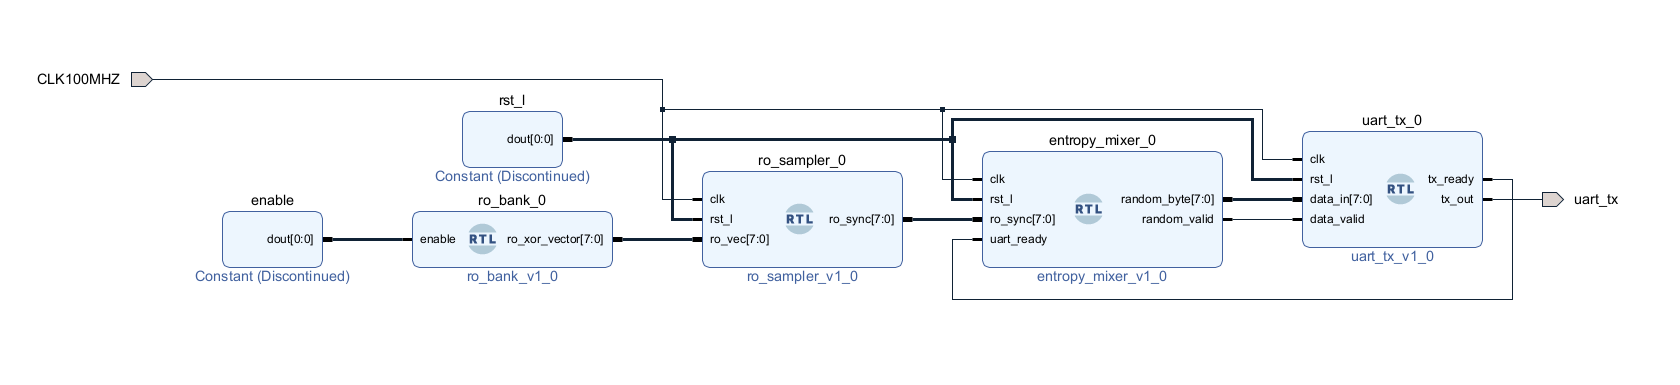
\includegraphics[width=1\textwidth]{gfx/block design}
    \caption{Block Design modułu nadrzędnego.}
    \label{fig:blockdesign}
\end{figure}

Istotną zaletą środowiska Vivado jest pełna kontrola nad strukturą
projektowanego układu oraz dostęp do raportów zasobowych,
co ma kluczowe znaczenie w przypadku oscylatorów pierścieniowych.
Niewielkie różnice w opóźnieniach propagacji bramek oraz sposób
rozmieszczenia logiki w strukturze FPGA mają bezpośredni wpływ na
właściwości generowanego sygnału i poziom entropii. Dodatkowo moduł nadrzędny
projektu, opisujący porty modułów HDL in/out bezpośrednio zmapowane do pinów fizycznego układu,
może być generowany z blokowego schematu który pozwala na dokładne zrozumienie data flow bez przeglądania
wielu linii kodu rys.\ref{fig:blockdesign}.

Jako platformę sprzętową wybrano płytkę rozwojową Arty S7-25 z układem
Xilinx Spartan-7. Jest to nowoczesny układ FPGA przeznaczony do aplikacji
o umiarkowanej złożoności, oferujący dobrą relację dostępnych zasobów
logicznych do poboru mocy i kosztu. Rodzina Spartan-7 zapewnia stabilne
parametry czasowe oraz powtarzalne zachowanie struktur logicznych, co
jest istotne w kontekście implementacji generatorów liczb losowych.

\begin{figure}[ht]
    \centering
    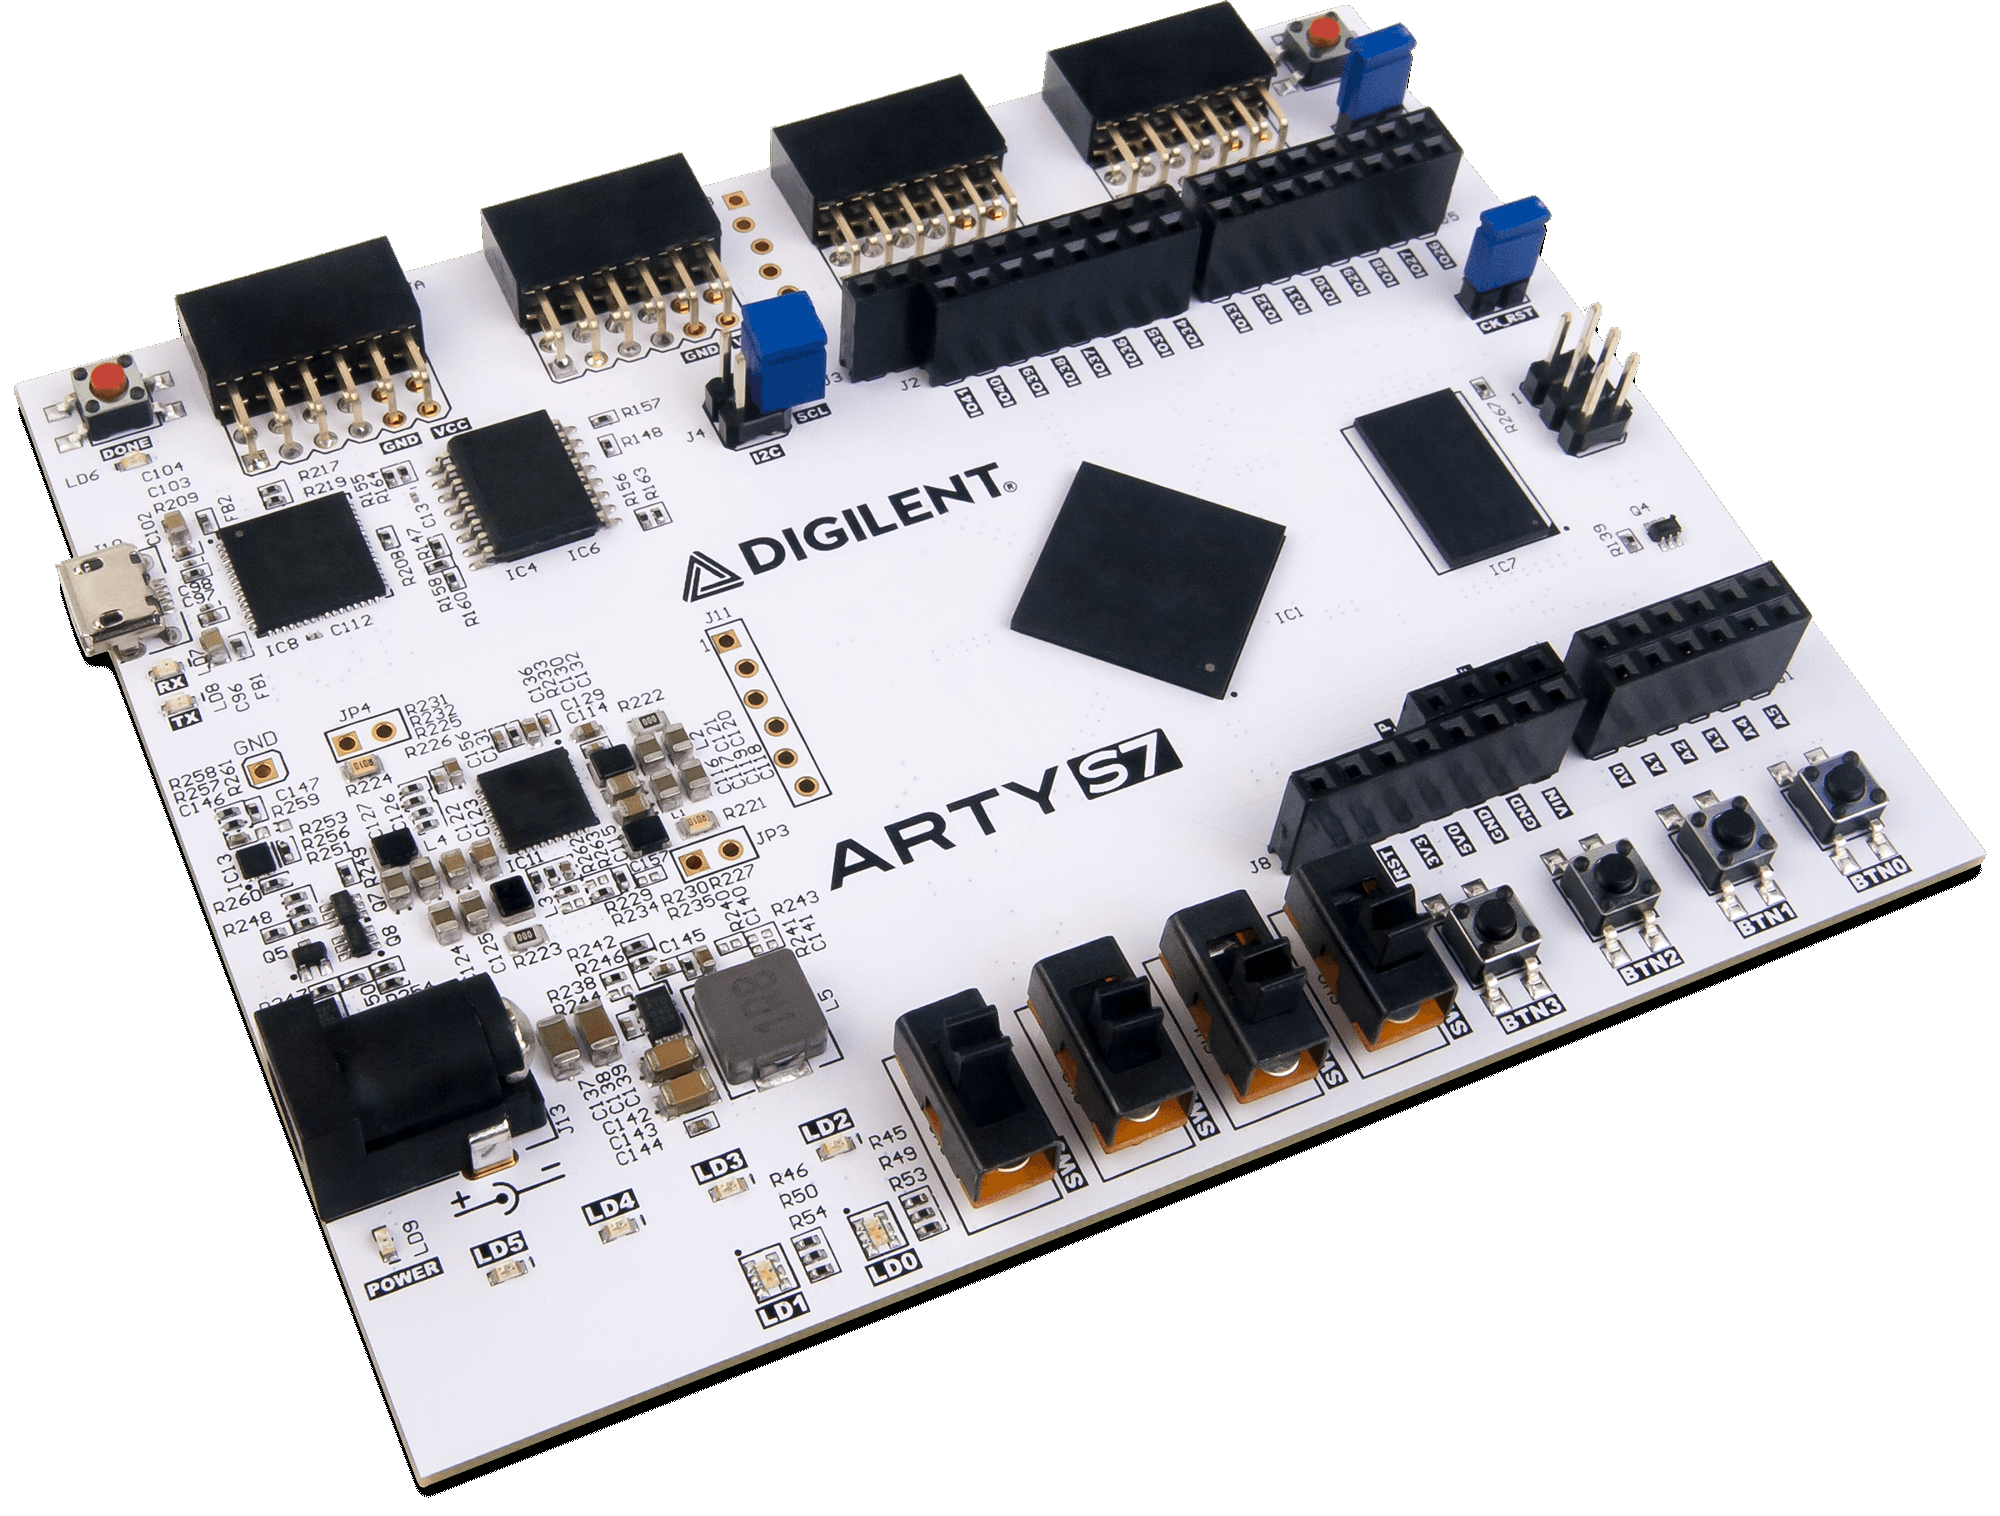
\includegraphics[width=0.75\textwidth]{gfx/board}
    \caption{Płytka ARTY S7-25, źródło: Digilent.com.}
    \label{fig:DevBoard}
\end{figure}

Dodatkowym argumentem przemawiającym za wyborem płytki Arty S7-25 jest jej
szerokie wsparcie narzędziowe oraz dostępność dokumentacji i przykładów
projektowych. Płytka posiada standardowy interfejs JTAG do programowania
i debugowania, co umożliwia wygodne testowanie implementacji oraz
obserwację zachowania układu w warunkach rzeczywistych.

\section{Implementacja oscylatora pierścieniowego w języku VHDL}

Podrozdział opisuje implementację oscylatora pierścieniowego, który jest
podstawowym blokiem generatora. Opis w języku VHDL przeznaczony jest do syntezy
w strukturze FPGA i składa się z trzech części: deklaracji biblioteki,
deklaracji jednostki oraz architektury opisującej logikę. Każda z nich
omówiona jest osobno.

\begin{lstlisting}[language=VHDL,
caption={Standardowe biblioteki VHDL (ring\_oscillator.vhdl)},
label={lst:ring_oscillator_lib}]
library IEEE;
use IEEE.STD_LOGIC_1164.ALL;
\end{lstlisting}

Listing \ref{lst:ring_oscillator_lib} zawiera deklarację biblioteki. Standard
VHDL udostępnia jedynie dwuwartościowy typ \texttt{bit}, dlatego dołączono
pakiet \texttt{IEEE.STD\_LOGIC\_1164}, który wprowadza wielowartościowy typ
\texttt{std\_logic} oraz jego wektorową odmianę \texttt{std\_logic\_vector}.
Typy te opisują porty \texttt{enable} i \texttt{ro\_out} oraz sygnał
wewnętrzny \texttt{w}. Pakiet definiuje także operatory logiczne, w tym negację \texttt{not}, użytą
do zbudowania łańcucha inwerterów. Ponieważ jest on standaryzowany przez IEEE,
kod pozostaje przenośny między narzędziami różnych producentów, a syntezator
interpretuje go jednoznacznie.

\begin{lstlisting}[language=VHDL,
caption={Moduł oscylatora pierścieniowego (ring\_oscillator.vhdl)},
label={lst:ring_oscillator_entity}]
entity ring_osc is
    generic (
        STAGES : positive := 7
    );
    port (
        enable : in  std_logic;
        ro_out : out std_logic
    );
    attribute dont_touch : string;
    attribute dont_touch of ring_osc : entity is "yes";
end ring_osc;
\end{lstlisting}

Listing \ref{lst:ring_oscillator_entity} przedstawia deklarację jednostki
\texttt{ring\_osc}, czyli interfejs modułu. Parametr generyczny
\texttt{STAGES} określa liczbę stopni inwersji i domyślnie wynosi 7. Liczba
ta musi być nieparzysta, ponieważ tylko wtedy pętla inwerterów nie ma
stabilnego stanu logicznego i wymusza ciągłe przełączanie. Zmiana wartości
parametru pozwala regulować częstotliwość oscylatora bez ingerencji
w strukturę kodu. Moduł ma dwa porty. Wejście \texttt{enable} steruje wyjściem, a na wyjściu
\texttt{ro\_out} dostępny jest przebieg oscylatora.
Atrybut \texttt{dont\_touch} przypisany do całej jednostki informuje narzędzia
syntezy \cite{amd_vivado_donttouch}, że moduł nie może być usuwany ani
upraszczany przez optymalizator. Dzięki temu każdy egzemplarz oscylatora
pozostaje w projekcie odrębną, nienaruszoną strukturą.

\begin{lstlisting}[language=VHDL,
caption={Logika oscylatora pierścieniowego (ring\_oscillator.vhdl)},
label={lst:ring_oscillator_logic}]
architecture RTL of ring_osc is
    signal w : std_logic_vector(STAGES-1 downto 0);

    attribute keep              : string;
    attribute dont_touch of w   : signal is "yes";
    attribute keep       of w   : signal is "true";
    attribute dont_touch of RTL : architecture is "yes";
begin
    w(0) <= not w(STAGES-1);

    gen_inv : for i in 1 to STAGES-1 generate
        w(i) <= not w(i-1);
    end generate;

    ro_out <= w(STAGES-1) when enable = '1' else '0';
end RTL;
\end{lstlisting}

Listing \ref{lst:ring_oscillator_logic} zawiera architekturę \texttt{RTL},
czyli opis logiki oscylatora. Jej rdzeniem jest wektor sygnałów \texttt{w}
o długości \texttt{STAGES}, w którym każdy element odpowiada wyjściu jednego
stopnia inwersji.

Kluczowe znaczenie mają atrybuty \texttt{dont\_touch} i \texttt{keep},
przypisane do sygnału \texttt{w}, a atrybut \texttt{dont\_touch} także do
architektury. Informują one narzędzia syntezy
\cite{amd_vivado_donttouch,amd_vivado_keep}, że pętla kombinacyjna jest
zamierzoną strukturą funkcjonalną, a nie błędem projektowym. Bez tej
deklaracji optymalizator mógłby usunąć lub uprościć logikę, traktując ją jako
zbędną lub niepoprawną. Atrybuty te zwiększają szansę zachowania fizycznej
struktury pierścienia w docelowym układzie FPGA, co jest warunkiem powstania
oscylacji.

Pętla sprzężenia zwrotnego zamyka się w przypisaniu
\texttt{w(0) <= not w(STAGES-1)}. Pierwszy stopień otrzymuje więc na wejście
zanegowany sygnał z ostatniego elementu łańcucha. Pozostałe stopnie powstają
w pętli \texttt{generate} i realizują prostą inwersję sygnału poprzedzającego.
W pętli znajduje się w sumie \texttt{STAGES} inwerterów.

Sygnał wyjściowy \texttt{ro\_out} jest pobierany z ostatniego stopnia łańcucha
i przekazywany na zewnątrz tylko wtedy, gdy \texttt{enable} ma wartość
\texttt{'1'}. W przeciwnym razie na wyjściu ustawiany jest stan \texttt{'0'}.
Sygnał \texttt{enable} nie przerywa zatem pętli, a jedynie bramkuje wyjście,
więc oscylator pracuje także wtedy, gdy wyjście jest wyłączone. Częstotliwość
przebiegu zależy od liczby stopni inwersji oraz od opóźnień propagacji
w danej technologii sprzętowej.

Całość architektury ma charakter czysto kombinacyjny i świadomie narusza
klasyczne zasady projektowania synchronicznego. Jest to konstrukcja
niskopoziomowa, silnie zależna od właściwości fizycznych układu docelowego,
a nie tylko od opisu logicznego.

\section{Implementacja generatora bitów losowych}

Generator składa się z dwóch bloków, które korzystają z oscylatora
\texttt{ring\_osc} opisanego wcześniej. Pierwszy z nich, moduł
\texttt{ro\_bank}, tworzy wiele instancji oscylatora i łączy ich wyjścia
w pary. Drugi, moduł \texttt{ro\_sampler}, próbkuje otrzymany wektor sygnałem
zegarowym i przekazuje go do dalszego przetwarzania. Każdy z modułów
omówiono w częściach odpowiadających kolejnym fragmentom kodu.

\subsection{Moduł banku oscylatorów}

\begin{lstlisting}[language=VHDL,
caption={Jednostka \texttt{ro\_bank} (\texttt{ro\_bank.vhdl})},
label={lst:ro_bank_entity}]
entity ro_bank is
    generic (OUT_WIDTH : positive := 8);
    port (
        enable        : in  std_logic;
        ro_xor_vector : out std_logic_vector(OUT_WIDTH - 1 downto 0)
    );
end entity ro_bank;
\end{lstlisting}

Listing \ref{lst:ro_bank_entity} przedstawia interfejs modułu. Parametr
generyczny \texttt{OUT\_WIDTH}, domyślnie równy 8, określa szerokość wektora
wyjściowego \texttt{ro\_xor\_vector}. Wejście \texttt{enable} jest globalnym
sygnałem włączającym dla wszystkich oscylatorów w banku.

\begin{lstlisting}[language=VHDL,
caption={Stałe i sygnały architektury \texttt{ro\_bank} (\texttt{ro\_bank.vhdl})},
label={lst:ro_bank_decl1}]
architecture rtl of ro_bank is
    constant RO_COUNT : positive := 2 * OUT_WIDTH;
    type stage_count_array is array (natural range <>) of positive;
    constant STAGE_TABLE : stage_count_array(0 to 15) := (7,  9, 11, 13, 15, 17, 19, 21, 23, 25, 27, 29, 31, 33, 35, 37);
    signal ro_vec : std_logic_vector(RO_COUNT - 1 downto 0);
\end{lstlisting}

Listing \ref{lst:ro_bank_decl1} rozpoczyna architekturę od deklaracji stałych
i sygnału. Na każdy bit wyjściowy przypadają dwa oscylatory, więc stała
\texttt{RO\_COUNT} wynosi $2\cdot\texttt{OUT\_WIDTH}$, a dla wartości domyślnej
powstaje 16 instancji. Ich wyjścia trafiają do wektora \texttt{ro\_vec}
o szerokości \texttt{RO\_COUNT}.

Tablica \texttt{STAGE\_TABLE} zawiera kolejne liczby nieparzyste od 7 do 37
i określa liczbę stopni inwersji każdego oscylatora. Im więcej stopni, tym
większe sumaryczne opóźnienie propagacji i tym niższa częstotliwość, więc
każdy sygnał w wektorze \texttt{ro\_vec} ma inną częstotliwość nominalną.
Ponieważ tablica ma 16 elementów, parametr \texttt{OUT\_WIDTH} nie może
przekraczać 8 bez jej rozszerzenia.

Statyczne różnice technologiczne między elementami układu dodatkowo
rozstrajają te częstotliwości, ale są stałe w czasie i nie stanowią źródła
entropii. Źródłem entropii są losowe zmiany opóźnień w czasie, czyli jitter
wynikający z szumu elektrycznego. Fluktuacje napięcia zasilania także
zmieniają opóźnienia, jednak mają składową deterministyczną, więc nie należy
ich traktować jako pewnego źródła losowości.

\begin{lstlisting}[language=VHDL,
caption={Atrybuty i komponent w architekturze \texttt{ro\_bank} (\texttt{ro\_bank.vhdl})},
label={lst:ro_bank_decl2}]
    attribute dont_touch : string;
    attribute keep       : string;
    component ring_osc is
        generic (STAGES : positive := 7);
        port (
            enable : in  std_logic;
            ro_out : out std_logic);
    end component ring_osc;
    attribute dont_touch of ring_osc      : component    is "yes";
    attribute dont_touch of ro_vec        : signal       is "yes";
    attribute keep       of ro_vec        : signal       is "true";
    attribute dont_touch of ro_xor_vector : signal       is "yes";
    attribute keep       of ro_xor_vector : signal       is "true";
    attribute dont_touch of rtl           : architecture is "yes";
\end{lstlisting}

Listing \ref{lst:ro_bank_decl2} kończy część deklaracyjną. Deklaracja
komponentu \texttt{ring\_osc} odtwarza interfejs jednostki z poprzedniego
podrozdziału, czyli parametr \texttt{STAGES} oraz porty \texttt{enable}
i \texttt{ro\_out}.

Atrybut \texttt{dont\_touch} przypisano komponentowi, sygnałom
\texttt{ro\_vec} i \texttt{ro\_xor\_vector} oraz całej architekturze,
a atrybut \texttt{keep} obu sygnałom. Bez nich syntezator mógłby uprościć
strukturę, usunąć pętle kombinacyjne lub połączyć logicznie równoważne
fragmenty \cite{amd_vivado_donttouch,amd_vivado_keep}. Generator opiera się na
fizycznych opóźnieniach bramek, więc takie optymalizacje zniszczyłyby jego
właściwości oscylacyjne.

\begin{lstlisting}[language=VHDL,
caption={Instancje oscylatorów i operacja XOR w architekturze \texttt{ro\_bank} (\texttt{ro\_bank.vhdl})},
label={lst:ro_bank_body}]
begin
    gen_ro : for i in 0 to RO_COUNT - 1 generate
        u_ro : ring_osc
            generic map (STAGES => STAGE_TABLE(i))
            port map (
                enable => enable,
                ro_out => ro_vec(i)
            );
    end generate gen_ro;
    gen_xor : for i in 0 to OUT_WIDTH - 1 generate
        ro_xor_vector(i) <= ro_vec(2 * i) xor ro_vec(2 * i + 1);
    end generate gen_xor;
end architecture rtl;
\end{lstlisting}

Listing \ref{lst:ro_bank_body} zawiera część wykonawczą architektury. Pętla
\texttt{gen\_ro} tworzy \texttt{RO\_COUNT} instancji oscylatora. Liczba stopni
każdej z nich jest pobierana z tablicy \texttt{STAGE\_TABLE} i przekazywana
parametrem \texttt{STAGES}, a wyjście trafia do kolejnego bitu wektora
\texttt{ro\_vec}. Sygnał \texttt{enable} jest doprowadzony do wszystkich
instancji. Tak jak w pojedynczym oscylatorze, steruje on wyłącznie
bramkowaniem wyjścia. Przy \texttt{enable = '0'} wektor
\texttt{ro\_xor\_vector} przyjmuje wartość zero, natomiast pętle inwerterów
pracują nadal.

Pętla \texttt{gen\_xor} łączy oscylatory w pary. Każdy bit
\texttt{ro\_xor\_vector(i)} jest wynikiem operacji różnicy symetrycznej
oscylatorów o numerach $2i$ i $2i+1$, a więc dla domyślnej tablicy par
o liczbie stopni (7, 9), (11, 13), (15, 17) i dalej aż do (35, 37).
Operacja ta łączy w jednym sygnale zmiany obu przebiegów, a tym samym jitter
obu oscylatorów. Wektor \texttt{ro\_vec} ma zatem 16 bitów, a wektor
wyjściowy 8. Nie należy przy tym zakładać, że oscylatory są wzajemnie
nieskorelowane. Wspólne zasilanie i przesłuchy w strukturze układu mogą je
sprzęgać, co jest jednym z zagadnień badanych w dalszej części pracy.

\subsection{Moduł próbkujący}

\begin{lstlisting}[language=VHDL,
caption={Jednostka \texttt{ro\_sampler} (\texttt{ro\_sampler.vhdl})},
label={lst:ro_sampler_entity}]
entity ro_sampler is
    port (
        clk     : in  std_logic;
        rst_l   : in  std_logic;
        ro_vec  : in  std_logic_vector(7 downto 0);
        ro_sync : out std_logic_vector(7 downto 0)
    );
end ro_sampler;
\end{lstlisting}

Listing \ref{lst:ro_sampler_entity} przedstawia interfejs modułu. Wejście
\texttt{clk} jest zegarem systemowym, a \texttt{rst\_l} asynchronicznym
resetem aktywnym stanem niskim. Do ośmiobitowego wejścia \texttt{ro\_vec}
doprowadzany jest wektor \texttt{ro\_xor\_vector} z modułu \texttt{ro\_bank},
a jego szerokość odpowiada domyślnej wartości parametru \texttt{OUT\_WIDTH}.
Wyjściem modułu jest wektor \texttt{ro\_sync} o tej samej szerokości.

\begin{lstlisting}[language=VHDL,
caption={Rejestry i atrybuty architektury \texttt{ro\_sampler} (\texttt{ro\_sampler.vhdl})},
label={lst:ro_sampler_decl}]
architecture RTL of ro_sampler is
    signal ff1, ff2 : std_logic_vector(7 downto 0);
    attribute ASYNC_REG, dont_touch, KEEP : string;
    attribute ASYNC_REG  of ff1, ff2 : signal is "TRUE";
    attribute dont_touch of ff1, ff2 : signal is "yes";
    attribute keep       of ff1, ff2 : signal is "true";
\end{lstlisting}

Listing \ref{lst:ro_sampler_decl} zawiera część deklaracyjną architektury.
Sygnały \texttt{ff1} i \texttt{ff2} są ośmiobitowymi rejestrami, które tworzą
dwustopniowy synchronizator.

Atrybut \texttt{ASYNC\_REG} informuje narzędzia implementacji, że rejestry
odbierają dane asynchroniczne i tworzą łańcuch synchronizujący
\cite{amd_vivado_asyncreg}. Atrybuty \texttt{dont\_touch} i \texttt{keep}
chronią je przed usunięciem, scaleniem lub optymalizacją zmieniającą ich
funkcję.

\begin{lstlisting}[language=VHDL,
caption={Proces próbkujący w architekturze \texttt{ro\_sampler} (\texttt{ro\_sampler.vhdl})},
label={lst:ro_sampler_body}]
begin
    process(clk, rst_l)
    begin
        if rst_l = '0' then
            ff1 <= (others => '0');
            ff2 <= (others => '0');
        elsif rising_edge(clk) then
            ff1 <= ro_vec;
            ff2 <= ff1;
        end if;
    end process;
    ro_sync <= ff2;
end RTL;
\end{lstlisting}

Listing \ref{lst:ro_sampler_body} zawiera część wykonawczą. Wejście
\texttt{ro\_vec} jest asynchroniczne względem zegara \texttt{clk}, więc nie
może być bezpośrednio przekazane do dalszej logiki sekwencyjnej. Na narastającym
zboczu zegara \texttt{ff1} przechwytuje aktualny stan wejścia, a \texttt{ff2}
przejmuje poprzednią zawartość \texttt{ff1}. Reset zeruje oba rejestry.

W tym generatorze próbkowanie asynchronicznego przebiegu zegarem jest
jednocześnie mechanizmem pozyskiwania entropii. Pierwszy przerzutnik zapisuje
chwilowy stan przebiegu, który zależy od fazy oscylatora, a więc także od
skumulowanego jitteru. Gdy zbocze wejścia trafi blisko krawędzi zegara,
przerzutnik może wejść w stan metastabilny, a drugi stopień ogranicza
ryzyko propagacji takiego stanu do dalszej części układu.

Sygnał \texttt{ro\_sync} jest zsynchronizowaną z domeną zegarową wersją
wektora \texttt{ro\_vec}. Jest gotowy do dalszej obróbki cyfrowej, na
przykład do detekcji zboczy i ekstrakcji bitów losowych.

\section{Implementacja modułu ekstrakcji entropii}

W niniejszym podrozdziale przedstawiono implementację modułu odpowiedzialnego za
przetworzenie surowych, spróbkowanych przebiegów z oscylatorów pierścieniowych w strumień
bajtów gotowych do wysłania interfejsem komunikacyjnym. Celem tego etapu projektu jest
oddzielenie warstwy generującej entropię od warstwy transmisyjnej, tak aby zmiana liczby
oscylatorów lub prędkości transmisji nie wymagała modyfikacji pozostałych elementów
układu. Wejściem modułu jest ośmiobitowy wektor \texttt{ro\_sync}, zawierający stany
wszystkich oscylatorów przeprowadzone uprzednio przez rejestry synchronizujące, co
eliminuje ryzyko propagacji stanów metastabilnych do dalszej części projektu. Cała logika
pracuje synchronicznie ze zboczem narastającym zegara systemowego, z synchronicznym
resetem aktywnym w stanie niskim (\texttt{rst\_l}). Kluczowy fragment implementacji
przedstawiono na listingu \ref{lst:entropy-extractor}.

\begin{lstlisting}[language=VHDL,
caption={Ekstrakcja bitów i buforowanie strumienia (entropy\_mixer.vhdl)},
label={lst:entropy-extractor}]
if have_first = '0' then
    prev_vec   <= ro_sync;
    have_first <= '1';
else
    fifo_v := bit_fifo;
    cnt_v  := fifo_count;

    for i in 0 to 7 loop
        if prev_vec(i) = '0' and ro_sync(i) = '1' then
            if cnt_v < 16 then
                fifo_v(cnt_v) := '0';
                cnt_v := cnt_v + 1;
            end if;
        elsif prev_vec(i) = '1' and ro_sync(i) = '0' then
            if cnt_v < 16 then
                fifo_v(cnt_v) := '1';
                cnt_v := cnt_v + 1;
            end if;
        end if;
    end loop;

    if cnt_v >= 8 and uart_ready = '1' then
        random_byte_r <= fifo_v(7 downto 0);
        valid_r       <= '1';

        for j in 0 to 7 loop
            fifo_v(j) := fifo_v(j + 8);
        end loop;
        for j in 8 to 15 loop
            fifo_v(j) := '0';
        end loop;

        cnt_v := cnt_v - 8;
    end if;

    bit_fifo   <= fifo_v;
    fifo_count <= cnt_v;
    have_first <= '0';
end if;
\end{lstlisting}

Ekstrakcja entropii opiera się na detekcji zboczy, a nie na bezpośrednim odczycie stanu
oscylatorów. Bieżący wektor \texttt{ro\_sync} porównywany jest z próbką poprzednią,
przechowywaną w rejestrze \texttt{prev\_vec}, przy czym dla każdego z ośmiu kanałów
niezależnie badana jest zmiana stanu: zbocze narastające interpretowane jest jako bit
o wartości \texttt{'0'}, zbocze opadające jako \texttt{'1'}, natomiast brak zmiany stanu
nie generuje żadnego bitu. Ponieważ dla każdego oscylatora zbocza narastające i opadające
muszą występować naprzemiennie, liczba wygenerowanych zer i jedynek pozostaje w dłuższym
przebiegu zrównoważona niezależnie od współczynnika wypełnienia sygnału. Odrzucenie
próbek, w których stan oscylatora nie zmienił się między kolejnymi taktami, eliminuje
ponadto najsilniej skorelowaną część strumienia wejściowego, powstającą przy próbkowaniu
oscylatora zegarem o zbyt wysokiej częstotliwości.

Znacznik \texttt{have\_first} po każdym cyklu porównania jest ponownie zerowany, w efekcie
czego moduł pracuje w rytmie dwutaktowym: w pierwszym takcie rejestrowana jest próbka
odniesienia, w drugim następuje porównanie i ekstrakcja bitów. Efektywna częstotliwość
próbkowania oscylatorów jest zatem dwukrotnie niższa od częstotliwości zegara
systemowego, a kolejne porównywane pary próbek nie zachodzą na siebie, co ogranicza
korelację między sąsiednimi bitami strumienia wyjściowego.

Pozyskane bity gromadzone są w szesnastobitowym buforze \texttt{bit\_fifo}, którego
zapełnienie śledzi licznik \texttt{fifo\_count}. Buforowanie jest konieczne, ponieważ
liczba bitów uzyskiwanych wjednym cyklu porównania jest zmienna i zależy od tego, ile
oscylatorów zmieniło stan - może wynosić od zera do ośmiu. Gdy w buforze znajduje się co
najmniej osiem bitów, a nadajnik zgłasza gotowość sygnałem \texttt{uart\_ready}, osiem
najstarszych bitów wystawiane jest na port \texttt{random\_byte} wraz z jednotaktowym
impulsem \texttt{random\_valid}, po czym zawartość bufora przesuwana jest o osiem pozycji,
a licznik odpowiednio zmniejszany. Warunkowanie transmisji flagą gotowości nadajnika
realizuje mechanizm handshake opisany w kolejnym podrozdziale i zapobiega
generowaniu bajtów szybciej, niż jest w stanie odebrać je interfejs komunikacyjny;
nadmiarowe bity pozostają w buforze do czasu zwolnienia nadajnika.

Przedstawiony moduł stanowi naturalne miejsce w ścieżce przetwarzania danych, w którym
można zaimplementować sprzętowe algorytmy korekcji rozkładu (ang. \emph{debiasing}).
Umieszczenie takiego bloku bezpośrednio przed nadajnikiem, a więc po ekstrakcji bitów
i przed ich serializacją do bajtów, jest rozwiązaniem korzystnym z dwóch powodów.
Po pierwsze, korekcja operuje wówczas na strumieniu bitowym o ustalonym formacie,
niezależnie od liczby użytych oscylatorów. Po drugie, algorytmy tej klasy charakteryzują
się zmienną przepustowością wyjściową, a obecny w module bufor pozwala pogodzić ją ze
stałą, ramkową naturą transmisji UART. Typowym przykładem jest korektor von Neumanna,
analizujący strumień w rozłącznych parach bitów: parę \texttt{01} zastępuje bitem
\texttt{'0'}, parę \texttt{10} bitem \texttt{'1'}, natomiast pary \texttt{00} i \texttt{11}
odrzuca w całości. Procedura ta usuwa systematyczne odchylenie prawdopodobieństwa
wystąpienia zera i jedynki, o ile kolejne bity są statystycznie niezależne, kosztem
redukcji przepustowości - w przypadku źródła nieobciążonego do około jednej czwartej
strumienia wejściowego. Zastosowany mechanizm detekcji zboczy realizuje częściowo
podobne zadanie, jednak w odniesieniu do pojedynczego kanału i w domenie czasu, przez co
nie usuwa korelacji między kanałami, implementacja algorytmu wybielania może zostać wykonana
również już po akwizycji danych z modułu nadajnika UART po stronie urządzenia docelowego.

\section{Implementacja protokołu UART do transmisji ciągu losowych bitow}

W niniejszym podrozdziale przedstawiono implementację protokołu UART, przeznaczoną do 
transmisji ciągu losowych bitów generowanych przez generator. Celem tego etapu 
projektu jest umożliwienie niezależnej, asynchronicznej komunikacji pomiędzy układem FPGA a 
systemem zewnętrznym, w którym dane losowe mogą być dalej przetwarzane lub analizowane. Moduł
jest parametryzowany przez parametr generic \texttt{clks\_per\_bit} decydujący o szybkości nadajnika (listing \ref{lst:uart_tx_entity}).

\begin{lstlisting}[language=VHDL,
caption={Entity UART TX (uart\_tx.vhdl)},
label={lst:uart_tx_entity}]
library IEEE;
use IEEE.STD_LOGIC_1164.ALL;
use IEEE.NUMERIC_STD.ALL;
-- clks_per_bit = CLK_FREQ / BAUD_RATE
-- 50 MHz:  9600 baud (5208),  19200 baud (2604), 38400 baud (1302),
--          57600 baud (868),  115200 baud (434)
entity uart_tx is
    generic (
        clks_per_bit : integer := 10417
    );
    port (
        clk        : in  std_logic;
        rst_l      : in  std_logic;
        data_in    : in  std_logic_vector(7 downto 0);
        data_valid : in  std_logic;
        tx_ready   : out std_logic;
        tx_out     : out std_logic
    );
end uart_tx;
\end{lstlisting}

Architektura modułu uart\_tx to typowy przykład maszyny stanów która stanowi podstawową konstrukcję w projektach
FPGA (listing \ref{lst:uart_tx}).
Nadajnik zrealizowano jako automat skończony (ang. \emph{finite state machine}, FSM)
o czterech stanach, z których każdy odpowiada kolejnej części ramki UART w formacie 8N1. 

W stanie \texttt{IDLE} linia \texttt{tx\_out}
utrzymywana jest w stanie wysokim, licznik \texttt{clk\_cnt} oraz wskaźnik bitu
\texttt{bit\_idx} są zerowane, a flaga \texttt{tx\_ready} sygnalizuje gotowość na przyjęcie
nowego bajtu. Wystawienie przez modułnadrzędny flagi \texttt{data\_valid} powoduje
zatrzaśnięcie danych w rejestrze \texttt{tx\_buf}, opuszczenie flagi gotowości i przejście
do stanu \texttt{START\_BIT}, w którym linia jest ściągana do zera na czas jednego okresu
bitowego - to zbocze opadające stanowi dla odbiornika znacznik początku transmitowanej ramki.

Stan \texttt{DATA\_BITS} wyprowadza na linię kolejne bity z rejestru \texttt{tx\_buf},
adresowane wskaźnikiem \texttt{bit\_idx}, począwszy od bitu najmniej znaczącego, zgodnie
z konwencją UART. Po ośmiu bitach automat przechodzi do stanu \texttt{STOP\_BIT}, w którym
linia wraca do stanu wysokiego na czas jednego bitu, po czym następuje powrót do
\texttt{IDLE} i ponowne zgłoszenie gotowości.

W każdym ze stanów odmierzanie czasu realizuje ten sam mechanizm: licznik \texttt{clk\_cnt}
jest inkrementowany do wartości \texttt{clks\_per\_bit-1}, a jego przepełnienie wyznacza
moment zmiany stanu. Parametr \texttt{clks\_per\_bit} stanowi iloraz częstotliwości zegara
systemowego i zadanej prędkości transmisji, dzięki czemu szybkość transmisji można zmienić
bez modyfikacji struktury automatu. Zastosowanie jednego wspólnego licznika dla wszystkich
faz ramki gwarantuje jednakowy czas trwania każdego bitu, co jest warunkiem poprawnego
próbkowania sygnału po stronie odbiornika.

Komunikację z pozostałymi modułami projektu oparto na mechanizmie handshake z użyciem flag
\texttt{data\_valid} i \texttt{tx\_ready}. Rozwiązanie to eliminuje konieczność
odmierzania czasu transmisji przez moduł nadrzędny - nowa dana może zostać wystawiona
wyłącznie wtedy, gdy nadajnik zgłasza gotowość, co zapobiega nadpisaniu zawartości rejestru
\texttt{tx\_buf} w trakcie trwania ramki i utracie danych.

\begin{lstlisting}[language=VHDL,
caption={UART TX State Machine (uart\_tx.vhdl)},
label={lst:uart_tx}]
case state is
    when IDLE =>
        tx_out   <= '1';
        tx_ready <= '1';
        clk_cnt  <= 0;
        bit_idx  <= 0;
        if data_valid = '1' then
            tx_buf  <= data_in;
            tx_ready <= '0';
            state   <= START_BIT;
        end if;
    when START_BIT =>
        tx_out <= '0';
        if clk_cnt < clks_per_bit-1 then
            clk_cnt <= clk_cnt + 1;
        else
            clk_cnt <= 0;
            state   <= DATA_BITS;
        end if;
    when DATA_BITS =>
        tx_out <= tx_buf(bit_idx);
        if clk_cnt < clks_per_bit-1 then
            clk_cnt <= clk_cnt + 1;
        else
            clk_cnt <= 0;
            if bit_idx < 7 then
                bit_idx <= bit_idx + 1;
            else
                bit_idx <= 0;
                state   <= STOP_BIT;
            end if;
        end if;
    when STOP_BIT =>
        tx_out <= '1';
        if clk_cnt < clks_per_bit-1 then
            clk_cnt <= clk_cnt + 1;
        else
            clk_cnt <= 0;
            state   <= IDLE;
        end if;
end case;
\end{lstlisting}
    \chapter{Badanie właściwości statystycznych generatora liczb losowych}

W niniejszym rozdziale przedstawiono praktyczną implementację metod statystycznych
zastosowanych do oceny jakości strumienia bitów wygenerowanego w układzie FPGA
z wykorzystaniem ring oscylatorów. Analiza została wykonana w języku Python na danych
zebranych z działającego układu. Celem badań było sprawdzenie, czy wygenerowany strumień
nie wykazuje zależności, które mogłyby świadczyć o występowaniu niepożądanych
powiązań pomiędzy kolejnymi próbkami.
Wyniki przedstawiono w postaci wykresów oraz tabel, co umożliwia ocenę
wizualną, jak i dokładne porównanie wartości liczbowych.

\section{Implementacja skryptów do akwizycji i analizy strumienia bitów}

W ramach pracy przygotowano zestaw skryptów w języku Python, których zadaniem jest
akwizycja danych z badanego układu oraz wykonanie podstawowych analiz statystycznych
zarejestrowanych strumieni bitów. Przyjęte rozwiązanie ma charakter modułowy.
Oznacza to, że część odpowiedzialna za konfigurację, wczytywanie danych, wstępne
przetwarzanie oraz właściwą analizę została rozdzielona na kilka plików, co
ułatwia rozwój kodu i wielokrotne powtarzanie eksperymentów.

\subsection{Moduł parametrów konfiguracyjnych}

Wspólna konfiguracja wszystkich programów została umieszczona w osobnym module
\texttt{user\_param.py}. Takie podejście pozwala oddzielić parametry konfiguracji
od kodu realizującego obliczenia. W praktyce oznacza to, że zmiana portu
szeregowego, liczby pobieranych bitów, maksymalnego opóźnienia autokorelacji
lub parametrów map dwuwymiarowych nie wymaga ingerencji w główną logikę programu.
Z punktu widzenia pracy badawczej jest to wygodne, ponieważ umożliwia szybkie
powtarzanie pomiarów dla różnych ustawień układu oraz porównywanie wyników
uzyskanych w różnych konfiguracjach.

Na listingu~\ref{lst:user_param_python} pokazano fragment modułu konfiguracyjnego.
Zawiera on zarówno parametry związane z transmisją UART, jak i ustawienia używane
w kolejnych etapach analizy.

\begin{lstlisting}[
    language=Python,
    caption={Fragment modułu konfiguracyjnego \texttt{user\_param.py}},
    label={lst:user_param_python},
    basicstyle=\ttfamily\small,
    breaklines=true,
    frame=single
]
UART_PORT = "COM11"
UART_BAUD = 9600
UART_TIMEOUT_S = 1.0
READ_CHUNK_SIZE = 4096
UART_BIT_ORDER = "msb"
CAPTURE_BITS = 10485760

MAX_LAG = 15
MAP2D_WORD_SIZES = (4, 8)
MAP2D_TAUS = tuple(range(9))
STEP = None
BIAS_ALPHA = 0.01
\end{lstlisting}

\subsection{Skrypt do akwizycji danych z interfejsu UART}

Pierwszym etapem procesu badawczego było zarejestrowanie strumienia bitów
generowanego przez układ sprzętowy. W tym celu opracowano skrypt
\texttt{uart\_capture.py}, którego zadaniem jest otwarcie portu szeregowego,
odbiór kolejnych porcji danych, konwersja bajtów do postaci bitowej oraz zapis
wyniku do pliku tekstowego.

Program pobiera dane w blokach o zadanym rozmiarze, a następnie rozpakowuje każdy odebrany
bajt do ośmiu bitów. Uwzględniono również możliwość wyboru kolejności bitów w bajcie,
co ma znaczenie przy współpracy z różnymi implementacjami sprzętowymi. Niezgodność
przyjętej konwencji z kolejnością wystawiania bitów przez nadajnik nie zmienia wprawdzie
zawartości informacyjnej strumienia, wprowadza jednak deterministyczną permutację pozycji
bitowych, która mogłaby zniekształcić wynik testów badających zależności lokalne.

Fragment implementacji przedstawiono w listingu\ref{lst:uart_capture_python}.
Widoczna funkcja realizuje odbiór kolejnych porcji danych i uzupełnianie tablicy
wynikowej aż do osiągnięcia zadanej długości strumienia. Tablica wynikowa alokowana jest
jednorazowo, przed rozpoczęciem odbioru, o docelowym rozmiarze \texttt{target\_bits},
dzięki czemu uniknięto wielokrotnej realokacji pamięci przy kolejnych iteracjach pętli.
Przy seriach rzędu milionów bitów ma to wymierny wpływ na czas akwizycji. Kolejne
fragmenty zapisywane są bezpośrednio w wyznaczonym wycinku tablicy, a zmienna
\texttt{collected} pełni funkcję wskaźnika bieżącej pozycji zapisu.

Istotnym elementem funkcji jest obsługa sytuacji, w których wywołanie \texttt{ser.read()}
zwraca pustą odpowiedź. Zdarza się to po upływie zdefiniowanego limitu czasu oczekiwania,
gdy generator chwilowo nie dostarcza danych, na przykład wtedy, gdy bufor modułu
ekstrakcji nie zgromadził jeszcze pełnego bajtu. Pusty odczyt nie jest wówczas traktowany
jako błąd, lecz powoduje jedynie ponowienie próby, co pozwala prowadzić akwizycję
niezależnie od zmiennej w czasie wydajności źródła entropii. Analogicznie pomijane są
porcje, z których dekoder nie zwrócił żadnych bitów.

Ostatni odebrany blok jest z reguły dłuższy niż liczba bitów pozostających do zebrania,
ponieważ rozmiar bloku nie musi być dzielnikiem zadanej długości serii. Zastosowanie
zmiennych \texttt{remaining} i \texttt{take} zapewnia przycięcie nadmiarowej części
i zakończenie akwizycji dokładnie na zadanej liczbie bitów. Ma to znaczenie dla
poprawności dalszej analizy, ponieważ część testów pakietu NIST wymaga strumienia
o ściśle określonej długości, a seria dłuższa od deklarowanej mogłaby prowadzić do
niejednoznacznego podziału danych na bloki.

\begin{lstlisting}[
    language=Python,
    caption={Fragment skryptu \texttt{uart\_capture.py} odpowiedzialny za akwizycję bitów},
    label={lst:uart_capture_python},
    basicstyle=\ttfamily\small,
    breaklines=true,
    frame=single
]
def capture_one_series(ser: serial.Serial, target_bits: int, 
    chunk_size: int, bit_order: str, 
    progress_every_percent: int,) -> np.ndarray:

    bits = np.empty(target_bits, dtype=np.uint8)
    collected = 0

    while collected < target_bits:
        raw = ser.read(chunk_size)
        if not raw:
            continue

        chunk_bits = decode_uart_chunk_to_bits(raw=raw, 
                     bit_order=bit_order)
        if chunk_bits.size == 0:
            continue

        remaining = target_bits - collected
        take = min(remaining, int(chunk_bits.size))
        bits[collected : collected + take] = chunk_bits[:take]
        collected += take

    return bits
\end{lstlisting}

\subsection{Skrypt wybielający z wykorzystaniem metody Von Neumanna}

Po rejestracji danych zastosowano dodatkowy etap wstępnego przetwarzania,
wybrano wybielanie strumienia bitów metodą Von Neumanna. Celem tego
algorytmu jest ograniczenie wpływu biasu, czyli nierównowagi pomiędzy liczbą
zer i jedynek, bez potrzeby stosowania bardziej złożonych metod korekcji.

Strumień wejściowy dzielony jest na kolejne
pary bitów. Jeżeli w parze wystąpią dwa identyczne bity, para jest odrzucana.
Jeżeli bity są różne, do strumienia wyjściowego przepisywany jest pierwszy bit
z tej pary. W efekcie otrzymywany jest nowy ciąg o lepszych właściwościach
statystycznych, chociaż zazwyczaj krótszy od ciągu wejściowego. Skuteczność metody
opiera się na założeniu, że kolejne bity strumienia są statystycznie niezależne,
a jedynym jego defektem jest stałe odchylenie prawdopodobieństwa. Przy spełnieniu
tego warunku obie różne pary występują z jednakowym prawdopodobieństwem niezależnie
od wartości biasu, co gwarantuje idealną równowagę strumienia wyjściowego. Ceną
jest redukcja długości ciągu, w przypadku źródła nieobciążonego do około jednej
czwartej liczby bitów wejściowych, a dla źródła silnie odchylonego jeszcze wyraźniejsza.
Z punktu widzenia pracy badawczej rozwiązanie to jest użyteczne, ponieważ pozwala
porównać wyniki analizy przed i po wybielaniu danych. Implementację tej operacji
przedstawiono na listingu\ref{lst:von_neumann_python}.

\begin{lstlisting}[
    language=Python,
    caption={Fragment skryptu \texttt{von\_neumann.py} realizującego wybielanie bitów},
    label={lst:von_neumann_python},
    basicstyle=\ttfamily\small,
    breaklines=true,
    frame=single
]
def von_neumann_whiten(bits: np.ndarray) -> np.ndarray:
    pair_count = len(bits) // 2
    if pair_count == 0:
        return np.empty(0, dtype=np.uint8)

    pairs = bits[: 2 * pair_count].reshape(pair_count, 2)
    different = pairs[:, 0] != pairs[:, 1]

    return pairs[different, 0].astype(np.uint8, copy=False)
\end{lstlisting}

Implementację zrealizowano w postaci wektorowej, bez jawnej pętli po parach bitów.
Liczba pełnych par wyznaczana jest przez dzielenie całkowite długości strumienia,
a przy nieparzystej liczbie bitów ostatni z nich jest pomijany, ponieważ nie tworzy
kompletnej pary. Operacja \texttt{reshape} przekształca jednowymiarową tablicę bitów
w macierz o dwóch kolumnach, w której każdy wiersz odpowiada jednej analizowanej parze.
Porównanie obu kolumn daje logiczną maskę wskazującą pary o różnych wartościach,
która następnie służy do wybrania z pierwszej kolumny wyłącznie bitów spełniających
warunek zachowania. Takie podejście pozwala przetworzyć całą serię pomiarową
w kilku operacjach na tablicach, co przy strumieniach rzędu milionów bitów jest
zauważalnie szybsze od przetwarzania iteracyjnego.

Wybielanie realizowane jest po stronie komputera, na danych już zarejestrowanych,
a nie w strukturze układu FPGA. Rozwiązanie takie przyjęto celowo, ponieważ umożliwia
ono wielokrotną analizę tej samej serii pomiarowej przy różnych ustawieniach przetwarzania
oraz bezpośrednie porównanie strumienia surowego z wybielonym. Warunek zwracający
tablicę pustą dla strumienia krótszego od dwóch bitów zabezpiecza dalsze etapy analizy
przed błędem przy przetwarzaniu niekompletnych serii.

\subsection{Skrypt do wyznaczania autokorelacji}

Skrypt \texttt{autocorrelation.py}, służy do oceny zależności pomiędzy
bitami oddzielonymi określonym opóźnieniem. Badanie autokorelacji jest istotne,
ponieważ pozwala sprawdzić, czy kolejne próbki są od siebie niezależne.
W idealnym generatorze liczb losowych wartości autokorelacji dla opóźnień
większych od zera powinny być bliskie zeru.

W analizowanym rozwiązaniu strumień wejściowy w postaci \texttt{0}/\texttt{1}
jest najpierw przekształcany do postaci \texttt{-1}/\texttt{+1}. Zabieg ten sprowadza
wartość oczekiwaną strumienia nieobciążonego do zera, dzięki czemu iloczyn dwóch
próbek przyjmuje wartość dodatnią przy zgodności bitów i ujemną przy ich
niezgodności, a średnia z takich iloczynów wprost wyraża siłę i znak zależności.
Przy oryginalnym kodowaniu zerojedynkowym iloczyn byłby niezerowy wyłącznie dla par
jedynek, co czyniłoby miarę nieczułą na znaczną część możliwych zależności. Następnie
dla każdego opóźnienia wyznaczana jest średnia wartość iloczynu dwóch fragmentów
ciągu, z których jeden jest przesunięty względem drugiego. Program realizuje
obliczenia dla opóźnień od zera do wartości określonej przez parametr
\texttt{MAX\_LAG}. Dodatkowo generowane są wykresy oraz tabela z obliczonymi
wartościami, co ułatwia interpretację wyników.

Przykładową implementację funkcji obliczającej autokorelację przedstawiono
na listingu\ref{lst:autocorrelation_python}.

\begin{lstlisting}[
    language=Python,
    caption={Fragment skryptu \texttt{autocorrelation.py} do wyznaczania autokorelacji},
    label={lst:autocorrelation_python},
    basicstyle=\ttfamily\small,
    breaklines=true,
    frame=single
]
def autocorrelation(bits: np.ndarray, max_lag: int) -> np.ndarray:
    if len(bits) < max_lag + 1:
        raise ValueError("Not enough bits for MAX_LAG.")

    x = bits.astype(np.int8) * 2 - 1
    ac = np.empty(max_lag + 1, dtype=np.float64)

    for lag in range(max_lag + 1):
        a = x[: len(x) - lag]
        b = x[lag:]
        ac[lag] = np.mean(a * b)

    return ac
\end{lstlisting}

Dla każdego opóźnienia tworzone są dwa wycinki tego samego ciągu, przesunięte
względem siebie o zadaną liczbę pozycji i skrócone do wspólnej długości, tak aby
uśrednianie obejmowało wyłącznie pary o pełnym pokryciu. Wynikiem funkcji jest
tablica o długości \texttt{MAX\_LAG+1}, w której pierwszy element odpowiada opóźnieniu
zerowemu. Element ten z definicji przyjmuje wartość jedności, ponieważ każda próbka
mnożona jest wówczas przez siebie samą, a wobec kodowania \texttt{-1}/\texttt{+1}
iloczyn ten jest zawsze dodatni. Stanowi to wygodny punkt odniesienia oraz prosty
test poprawności działania funkcji.

Interpretacja pozostałych wartości wymaga uwzględnienia rozrzutu statystycznego.
Nawet dla źródła idealnie losowego wyznaczone współczynniki nie są dokładnie zerowe,
lecz wahają się w otoczeniu zera z odchyleniem standardowym rzędu odwrotności
pierwiastka z liczby analizowanych par. Przy serii o długości miliona bitów oznacza
to typowe odchylenia rzędu jednej tysięcznej, wobec czego dopiero wartości istotnie
przekraczające ten poziom świadczą o rzeczywistej zależności między próbkami.
W przypadku badanego generatora szczególnej uwagi wymagają opóźnienia odpowiadające
liczbie oscylatorów oraz wielokrotności długości bajtu, ponieważ ewentualna
periodyczność wynikająca ze stałej kolejności zapisu kanałów do bufora ujawniłaby się
właśnie w tych miejscach.

Zastosowany algorytm ma złożoność proporcjonalną do iloczynu długości strumienia
i maksymalnego opóźnienia, co przy dużych wartościach parametru \texttt{MAX\_LAG}
może być kosztowne obliczeniowo. Dla rozważanych zakresów opóźnień narzut ten
pozostaje jednak akceptowalny, a bezpośrednia postać obliczeń jest czytelniejsza
i łatwiejsza do weryfikacji niż realizacja z użyciem szybkiej transformaty Fouriera.

\subsection{Skrypt do tworzenia dwuwymiarowych map opóźnień}

Do bardziej zaawansowanej analizy zależności w danych wykorzystano skrypt
\texttt{map2d\_analysis.py}. Jego zadaniem jest budowa dwuwymiarowych map
opóźnień, które pozwalają ocenić strukturę badanego strumienia z większą
dokładnością niż proste zliczanie zer i jedynek, czy autokorelacja pierwszego
rzędu. Miary jednowymiarowe wykrywają wyłącznie zależności liniowe pomiędzy
pojedynczymi bitami, wobec czego strumień może uzyskać poprawny wynik testu
autokorelacji, zawierając jednocześnie wyraźne prawidłowości na poziomie całych
słów.

Działanie programu polega na podziale strumienia bitów na słowa o zadanej długości,
na przykład 4 lub 8-bitowe, a następnie na utworzeniu par \((w[n], w[n+\tau])\)
dla wybranych wartości opóźnienia \(\tau\). Dla takich par wyznaczany jest
histogram dwuwymiarowy, który można interpretować jako mapę gęstości występowania
określonych kombinacji słów. Dla źródła idealnie losowego wszystkie kombinacje są
jednakowo prawdopodobne, wobec czego mapa powinna mieć charakter równomiernego
szumu, bez wyróżnionych linii, skupień ani obszarów pustych. Struktury regularne
widoczne na mapie świadczą o tym, że wartość danego słowa niesie informację
o wartości słowa następnego. Dodatkowo skrypt oblicza kilka prostych parametrów
opisujących taką mapę, między innymi liczbę zajętych komórek histogramu,
udział wypełnienia siatki oraz udział punktów leżących na przekątnej.
Pierwsze dwa parametry pozwalają stwierdzić, czy generator wykorzystuje całą
dostępną przestrzeń wartości, natomiast udział punktów na przekątnej wskazuje,
jak często słowo powtarza się po zadanym opóźnieniu, co jest bezpośrednią miarą
skłonności układu do zapadania w stany okresowe.
Wyniki te są zapisywane zarówno w postaci wykresów, jak i tabel zbiorczych.

Przykładowy fragment kodu generującego mapę 2D przedstawiono
w Listingu~\ref{lst:map2d_python}.

\begin{lstlisting}[
    language=Python,
    caption={Fragment skryptu \texttt{map2d\_analysis.py} generującego mapę opóźnień 2D},
    label={lst:map2d_python},
    basicstyle=\ttfamily\small,
    breaklines=true,
    frame=single
]
def plot_delay_map_2d(
        x: np.ndarray, y: np.ndarray,
        bit_count: int, word_count: int,
        word_size: int, tau: int,
        bins: int | None = None,
        output: Path | None = None,
    ) -> dict[str, int | float]: 

    max_val = 2**word_size
    if bins is None:
        bins = min(max_val, 256)

    hist, xedges, yedges = np.histogram2d(x, y, bins=bins,
        range=[[0, max_val], [0, max_val]],
    )

    occupied_bins = int(np.count_nonzero(hist))
    fill_ratio = occupied_bins / int(hist.size)
    diagonal_share = float(np.trace(hist)) / len(x)

    return {
        "word_size": word_size,
        "tau": tau,
        "occupied_bins": occupied_bins,
        "fill_ratio": fill_ratio,
        "diagonal_share": diagonal_share,
    }
\end{lstlisting}

Zakres histogramu wyznaczany jest na podstawie długości słowa i obejmuje pełny
przedział możliwych wartości. Liczba przedziałów podziału ustalana jest domyślnie
jako mniejsza z dwóch wartości: liczby możliwych kombinacji oraz górnego
ograniczenia równego 256. Dla słów czterobitowych oznacza to podział dokładnie
odwzorowujący pojedyncze wartości, natomiast dla słów dłuższych kilka sąsiednich
wartości trafia do wspólnej komórki. Ograniczenie to jest niezbędne z uwagi na
rozmiar histogramu, który rośnie z kwadratem liczby przedziałów, wymaga jednak
uwzględnienia przy interpretacji parametru wypełnienia. Przy zbyt dużej liczbie
komórek w stosunku do długości serii pomiarowej niski współczynnik wypełnienia
wynika bowiem z niedostatecznej liczby próbek, a nie z wadliwości generatora.

Udział punktów leżących na przekątnej wyznaczany jest jako iloraz śladu macierzy
histogramu i całkowitej liczby analizowanych par. Interpretacja tej wielkości
wymaga porównania z wartością oczekiwaną dla źródła losowego, która jest równa
odwrotności liczby przedziałów podziału. Wartość istotnie wyższa świadczy
o powtarzalności słów, natomiast wyraźnie niższa może wskazywać na mechanizm
wykluczający powtórzenia, co również stanowi odstępstwo od losowości.

Zastosowanie map dwuwymiarowych było przydatne z praktycznego punktu widzenia,
ponieważ pozwalało wykrywać nie tylko prosty bias, ale również bardziej złożone
zależności pomiędzy kolejnymi fragmentami badanego ciągu.

\subsection{Skrypt do wyznaczania odchylenia rozkładu bitów}

Skrypt \texttt{bias.py} służy do oceny najbardziej podstawowej właściwości strumienia
losowego, jaką jest równowaga pomiędzy liczbą zer i jedynek. Dla źródła idealnego
prawdopodobieństwo wystąpienia obu wartości jest jednakowe, wobec czego udział jedynek
w dostatecznie długim strumieniu powinien być bliski jednej drugiej. Odstępstwo od tej
wartości, określane jako odchylenie rozkładu lub bias, jest w przypadku generatorów
sprzętowych zjawiskiem oczekiwanym i wynika między innymi z niesymetrycznych czasów
propagacji zbocza narastającego i opadającego w łańcuchu inwerterów oraz z niezerowego
współczynnika wypełnienia próbkowanego przebiegu.

Program wczytuje strumienie bitów z pliku tekstowego, sprawdza poprawność danych
wejściowych, a następnie dla każdego strumienia wyznacza liczbę zer i jedynek,
prawdopodobieństwa $P(0)$ oraz $P(1)$, wartość biasu zdefiniowaną jako $P(1)-0{,}5$,
średnią po odwzorowaniu bitów do zbioru $\{-1,+1\}$, a także wartość $p$ dla testu
monobitowego. Poziom istotności zadawany jest w konfiguracji parametrem
\texttt{BIAS\_ALPHA}, dzięki czemu procedurę można powtarzać dla różnych ustawień.
Fragment implementacji przedstawiono na listingu~\ref{lst:bias_python}.

\begin{lstlisting}[
    language=Python,
    caption={Fragment skryptu realizującego analizę biasu strumienia bitów},
    label={lst:bias_python},
    basicstyle=\ttfamily\small,
    breaklines=true,
    frame=single
]
def analyze_bitstream(bits: np.ndarray, bitstream_idx: int, bitstream_count: int) -> dict[str, float | int | bool]:
    total_bits = len(bits)
    one_count = int(np.count_nonzero(bits))
    zero_count = total_bits - one_count
    p_one = one_count / total_bits
    p_zero = zero_count / total_bits
    bias_01 = p_one - 0.5
    mean_pm1 = 2.0 * p_one - 1.0
    sigma_bias = 0.5 / sqrt(total_bits)
    s_n = one_count - zero_count
    s_obs = abs(s_n) / sqrt(total_bits)
    p_value = erfc(s_obs / sqrt(2.0))
    passed = p_value >= BIAS_ALPHA

    return {
        "bitstream_idx": bitstream_idx, "total_bits": total_bits,
        "zero_count": zero_count, "one_count": one_count,
        "p_zero": p_zero, "p_one": p_one,
        "bias_01": bias_01, "mean_pm1": mean_pm1,
        "sigma_bias": sigma_bias, "p_value": p_value,
        "passed": passed,
    }
\end{lstlisting}

Liczba jedynek wyznaczana jest jednym wywołaniem funkcji zliczającej elementy niezerowe,
co przy strumieniach rzędu milionów bitów jest znacznie szybsze od przetwarzania
iteracyjnego. Obie zwracane miary odchylenia, $P(1)-0{,}5$ oraz średnia w kodowaniu
$\{-1,+1\}$, opisują to samo zjawisko i różnią się wyłącznie skalą, przy czym druga
z nich jest dokładnie dwukrotnie większa. Podanie obu wynika z tego, że pierwsza jest
przyjęta w opisach generatorów sprzętowych, natomiast druga pojawia się w kontekście
analizy korelacyjnej, gdzie stosuje się to samo odwzorowanie bitów.

Kluczowym elementem funkcji jest realizacja testu monobitowego zgodnie z metodyką
pakietu NIST. Wyznaczana jest nadwyżka jedynek nad zerami, normowana pierwiastkiem
z długości strumienia, a otrzymana statystyka przeliczana jest na wartość $p$ przy użyciu
uzupełniającej funkcji błędu. Wartość ta określa prawdopodobieństwo zaobserwowania
odchylenia co najmniej tak dużego, jak stwierdzone, przy założeniu że źródło jest
idealnie zrównoważone. Normowanie długością serii jest tu istotne dla interpretacji
wyników: ta sama wartość biasu daje tym mniejszą wartość $p$, im dłuższa jest analizowana
seria, ponieważ dłuższa próba pozwala wykryć coraz subtelniejsze odchylenia. Wyznaczane
dodatkowo odchylenie standardowe $\sigma = 1/(2\sqrt{N})$ służy jako miara odniesienia
i pozwala wyrazić stwierdzone odstępstwo w jednostkach naturalnego rozrzutu
statystycznego.

\subsection{Podsumowanie}

Przygotowany zestaw skryptów tworzy spójne środowisko do badań nad jakością
strumienia bitów generowanego przez badany układ. Skrypt \texttt{uart\_capture.py}
odpowiada za akwizycję danych, moduł \texttt{user\_param.py} zapewniają wspólną 
konfigurację, \texttt{von\_neumann.py} realizuje wstępne wybielanie strumienia, natomiast
\texttt{autocorrelation.py}, \texttt{bias.py} oraz \texttt{map2d\_analysis.py}
służą do właściwej analizy statystycznej. Taki podział ułatwia zarówno
powtarzanie eksperymentów, jak i porównywanie wyników uzyskanych dla różnych
konfiguracji generatora.

Przyjęta struktura odzwierciedla naturalną kolejność przetwarzania danych,
od akwizycji, przez opcjonalne wybielanie, aż do analizy statystycznej. Rozdzielenie
tych etapów sprawia, że pojedyncza seria pomiarowa, po jednorazowym zarejestrowaniu,
może być poddawana wielokrotnej analizie przy różnych ustawieniach parametrów, bez
konieczności ponownego uruchamiania układu sprzętowego. Wydzielenie parametrów
konfiguracyjnych do osobnego modułu zapewnia ponadto, że wszystkie skrypty
operują na jednakowych ustawieniach długości serii, kolejności bitów oraz
zakresów analizy, co jest warunkiem porównywalności wyników uzyskanych
w kolejnych eksperymentach.

Zastosowane miary są wobec siebie komplementarne. Analiza biasu ocenia rozkład
wartości pojedynczych bitów, autokorelacja bada zależności między bitami
oddalonymi o zadaną liczbę pozycji, natomiast mapy dwuwymiarowe ujawniają
prawidłowości na poziomie całych słów. Dopiero łączne rozpatrzenie wyników
wszystkich trzech metod, dla strumienia surowego oraz wybielonego, pozwala
formułować wnioski na temat jakości badanego źródła entropii.

\subsection{Zestawienie parametrów badanych konfiguracji}

Wszystkie omówione pomiary wykonano na tej samej płytce rozwojowej i przy jednakowej
długości serii pomiarowej wynoszącej $10\,485\,760$ bitów, co odpowiada dziesięciu
mebibajtom danych. Konfiguracje różniły się liczbą użytych oscylatorów, sposobem ich
rozmieszczenia w strukturze układu, obecnością operacji XOR na wyjściach oraz
zastosowaniem wybielania po stronie komputera. Zestawienie tych parametrów przedstawiono
w tabeli~\ref{tab:konfiguracje}.

\begin{table}[htbp]
    \centering
    \caption{Parametry badanych konfiguracji generatora}
    \label{tab:konfiguracje}
    \small
    \begin{tabular}{clcccc}
        \toprule
        Nr & Rozmieszczenie & Liczba RO & Kanały & XOR & Wybielanie \\
        \midrule
        1 & automatyczne & 8  & 8 & nie  & nie \\
        2 & ręczne       & 8  & 8 & nie  & nie \\
        3 & ręczne       & 16 & 8 & tak  & nie \\
        4 & ręczne       & 16 & 8 & tak  & tak \\
        \bottomrule
    \end{tabular}
\end{table}

Liczba stopni inwersji poszczególnych oscylatorów została ustalona w tablicy stałych
\texttt{STAGE\_TABLE} i wynosi kolejno od 7 do 37, ze skokiem równym dwa. Zastosowanie
wyłącznie wartości nieparzystych jest warunkiem koniecznym wystąpienia oscylacji,
ponieważ przy parzystej liczbie inwerterów pętla sprzężenia zwrotnego realizowałaby
funkcję tożsamości i układ ustaliłby się w jednym ze stanów stabilnych. Zróżnicowanie
długości łańcuchów prowadzi natomiast do zróżnicowania częstotliwości pracy, która maleje
w przybliżeniu odwrotnie proporcjonalnie do liczby stopni. Zapobiega to sytuacji,
w której wszystkie oscylatory pracowałyby z jednakową częstotliwością nominalną, co
zwiększałoby ryzyko ich wzajemnej synchronizacji i ograniczyłoby efektywną liczbę
niezależnych źródeł szumu.

W konfiguracjach obejmujących osiem oscylatorów wykorzystywanych jest osiem pierwszych
pozycji tablicy, a więc łańcuchy o długościach od 7 do 21 stopni. W konfiguracjach
z szesnastoma oscylatorami wykorzystywana jest cała tablica, przy czym wyjścia łączone są
w pary operacją XOR według schematu 0--1, 2--3 i tak dalej, do pary 14--15. Do modułu
ekstrakcji entropii doprowadzonych jest zatem w każdym przypadku osiem sygnałów,
co oznacza, że przepustowość generatora nie zależy od liczby zaimplementowanych
oscylatorów. Warto zwrócić uwagę, że przyjęty schemat parowania zestawia zawsze łańcuch
krótszy z łańcuchem o dwa stopnie dłuższym, a więc o najbliższej możliwej częstotliwości
w obrębie zestawu.

Rozmieszczenie oscylatorów w konfiguracjach 2--4 narzucono ręcznie za pomocą ograniczeń
\texttt{LOC} oraz \texttt{BEL} zapisanych w pliku ograniczeń projektu. Pierwsze
z~ograniczeń przypisuje dany element logiczny do konkretnego bloku \texttt{SLICE},
drugie wskazuje wybrany generator funkcji w obrębie tego bloku. Takie podejście pozwala
uzyskać powtarzalną implementację, niezależną od kolejnych przebiegów narzędzia
rozmieszczającego, co jest warunkiem porównywalności pomiarów wykonanych w~różnym czasie.
Obszary zajmowane przez poszczególne oscylatory zestawiono w~tabeli~\ref{tab:rozm},
podając zakres współrzędnych bloków, w~których umieszczono należące do nich generatory
funkcji.

\begin{table}[htbp]
    \centering
    \caption{Liczba stopni inwersji oraz obszar rozmieszczenia poszczególnych oscylatorów}
    \label{tab:rozm}
    \small
    \begin{tabular}{ccccccc}
        \toprule
        RO & Stopnie & Obszar & \phantom{aa} & RO & Stopnie & Obszar \\
        \midrule
        0 & 7  & X40Y1--X40Y2   & & 8  & 23 & X0Y48--X2Y49   \\
        1 & 9  & X0Y99--X1Y99   & & 9  & 25 & X16Y48--X19Y49 \\
        2 & 11 & X6Y97--X7Y97   & & 10 & 27 & X35Y40--X40Y42 \\
        3 & 13 & X22Y0--X23Y2   & & 11 & 29 & X23Y87--X28Y89 \\
        4 & 15 & X19Y15--X22Y16 & & 12 & 31 & X5Y37--X8Y38   \\
        5 & 17 & X31Y67--X33Y68 & & 13 & 33 & X10Y63--X15Y64 \\
        6 & 19 & X31Y97--X32Y99 & & 14 & 35 & X33Y24--X36Y26 \\
        7 & 21 & X4Y73--X7Y74   & & 15 & 37 & X6Y84--X10Y87  \\
        \bottomrule
    \end{tabular}
\end{table}

\begin{figure}[htbp]
    \centering
    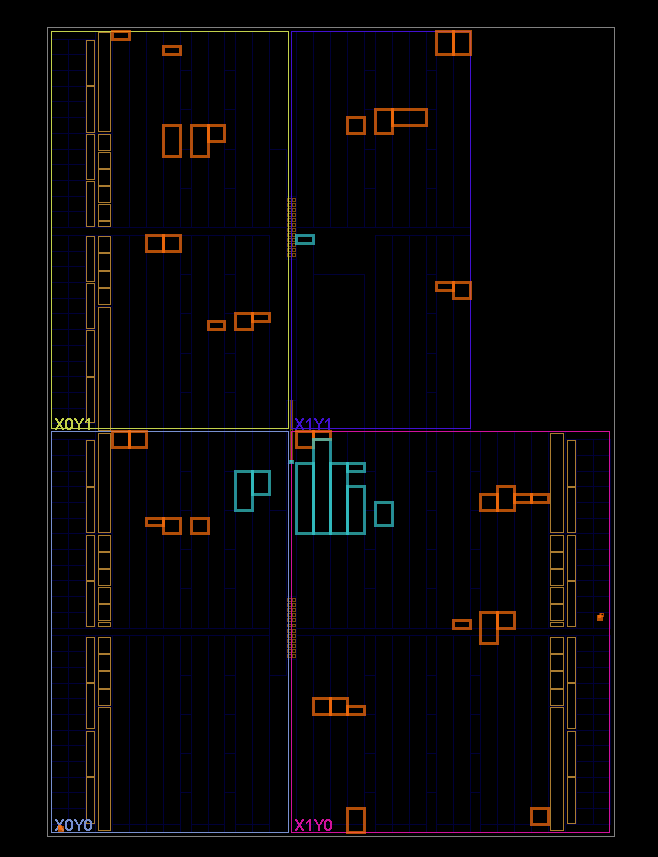
\includegraphics[width=0.7\textwidth]{gfx/ro_trng_xor_place_and_route.png}
    \caption{Widok struktury układu Spartan-7 po etapie rozmieszczenia i trasowania dla
    konfiguracji z 16 oscylatorami. Kolorem pomarańczowym oznaczono zasoby zajęte przez
    oscylatory pierścieniowe, kolorem błękitnym logikę modułu ekstrakcji entropii oraz
    nadajnika UART. Podpisy w narożnikach wskazują granice regionów zegarowych}
    \label{fig:place_and_route}
\end{figure}

Efekt zastosowanych ograniczeń przedstawiono na rysunku~\ref{fig:place_and_route},
obrazującym rozmieszczenie logiki w strukturze układu po etapie implementacji.
Oscylatory zajmują niewielkie, wyraźnie odseparowane grupy bloków rozproszone po całej
powierzchni logiki programowalnej, obejmujące wszystkie cztery regiony zegarowe układu.
Widoczne jest przy tym zróżnicowanie rozmiaru poszczególnych grup, wynikające
bezpośrednio z liczby stopni inwersji: łańcuchy najkrótsze mieszczą się w obrębie jednego
lub dwóch bloków, natomiast łańcuchy o kilkudziesięciu stopniach zajmują kilka bloków
sąsiadujących w poziomie. Zwarta grupa w centralnej części struktury odpowiada logice
synchronicznej projektu, a więc modułowi ekstrakcji entropii, nadajnikowi UART oraz
rejestrom synchronizującym.

Podział struktury na regiony zegarowe jest istotny z punktu widzenia niezależności
źródeł entropii, ponieważ każdy region posiada odrębne zasoby dystrybucji sygnału
zegarowego oraz własne punkty przyłączenia do sieci zasilania. Rozmieszczenie
oscylatorów w różnych regionach zwiększa zatem prawdopodobieństwo, że lokalne
zaburzenia napięcia zasilania, wywołane przełączaniem logiki synchronicznej, będą
oddziaływać na poszczególne pierścienie w sposób nieskorelowany. Jednocześnie warto
zaznaczyć, że żaden z oscylatorów nie został umieszczony w bezpośrednim sąsiedztwie
logiki synchronicznej, co ogranicza wpływ jej okresowej aktywności na częstotliwość
generowanych przebiegów.

Przyjęte rozmieszczenie obejmuje praktycznie cały obszar logiki programowalnej układu,
od bloków o najniższych współrzędnych po skrajne bloki w~narożnikach struktury. Oscylatory
tworzące jedną parę połączoną operacją XOR umieszczono w~odległych obszarach, przy czym
w~skrajnym przypadku pary 0--1 są to przeciwległe narożniki układu. Wyjątkiem jest para
8--9, której oba oscylatory znajdują się w~tym samym pasie poziomym, w~odległości około
szesnastu bloków. Konfiguracja ta jest zatem najbardziej narażona na wzajemne
oddziaływanie obu struktur i stanowi potencjalne źródło osłabienia skuteczności operacji
XOR dla tego kanału.

Łączne zapotrzebowanie na zasoby logiczne wynika bezpośrednio z~liczby stopni inwersji.
Każdy stopień realizowany jest przez jeden generator funkcji, a~dodatkowy generator
w~każdym oscylatorze pełni funkcję bramkowania sygnału wyjściowego sygnałem zezwolenia.
Konfiguracje z~ośmioma oscylatorami wymagają zatem 120 generatorów funkcji, natomiast
konfiguracje z~szesnastoma oscylatorami 368, nie licząc logiki modułu ekstrakcji entropii
oraz nadajnika UART. Struktury oscylatorów objęto atrybutami \texttt{dont\_touch} oraz
\texttt{keep}, co uniemożliwia narzędziu syntezy usunięcie łańcucha inwerterów jako
logiki redundantnej lub jego uproszczenie do pojedynczej negacji.

\FloatBarrier

\section{Badanie autokorelacji uzyskanych strumieni bitów}

Jednym z pierwszych wykonanych badań była analiza autokorelacji wygenerowanego strumienia
bitów. W praktyce test ten został użyty do sprawdzenia, czy kolejne bity wygenerowane w
układzie FPGA nie wykazują krótkookresowych zależności, które mogłyby wynikać z architektury
układu, sposobu próbkowania lub zbyt małego poziomu entropii na wejściu bloku
odpowiedzialnego za generację bitów. Do badania wykorzystano zapisany strumień o długości
$10\,485\,760$ bitów. Analiza została wykonana dla opóźnień od 0 do 15. Obliczenia
zrealizowano w języku Python, a skrypt został przygotowany tak, aby automatycznie wyznaczać
współczynniki autokorelacji oraz zapisywać wyniki w postaci wykresu i tabeli.

\subsection{Wyniki pomiaru dla 8 oscylatorów bez wybielania}

Przebieg współczynnika autokorelacji w funkcji opóźnienia przedstawiono na
rysunku~\ref{fig:autokorelacja_bitstream}, natomiast dokładne wartości liczbowe zestawiono
w tabeli~\ref{tab:autokorelacja_wyniki}.

\begin{figure}[htbp]
    \centering
    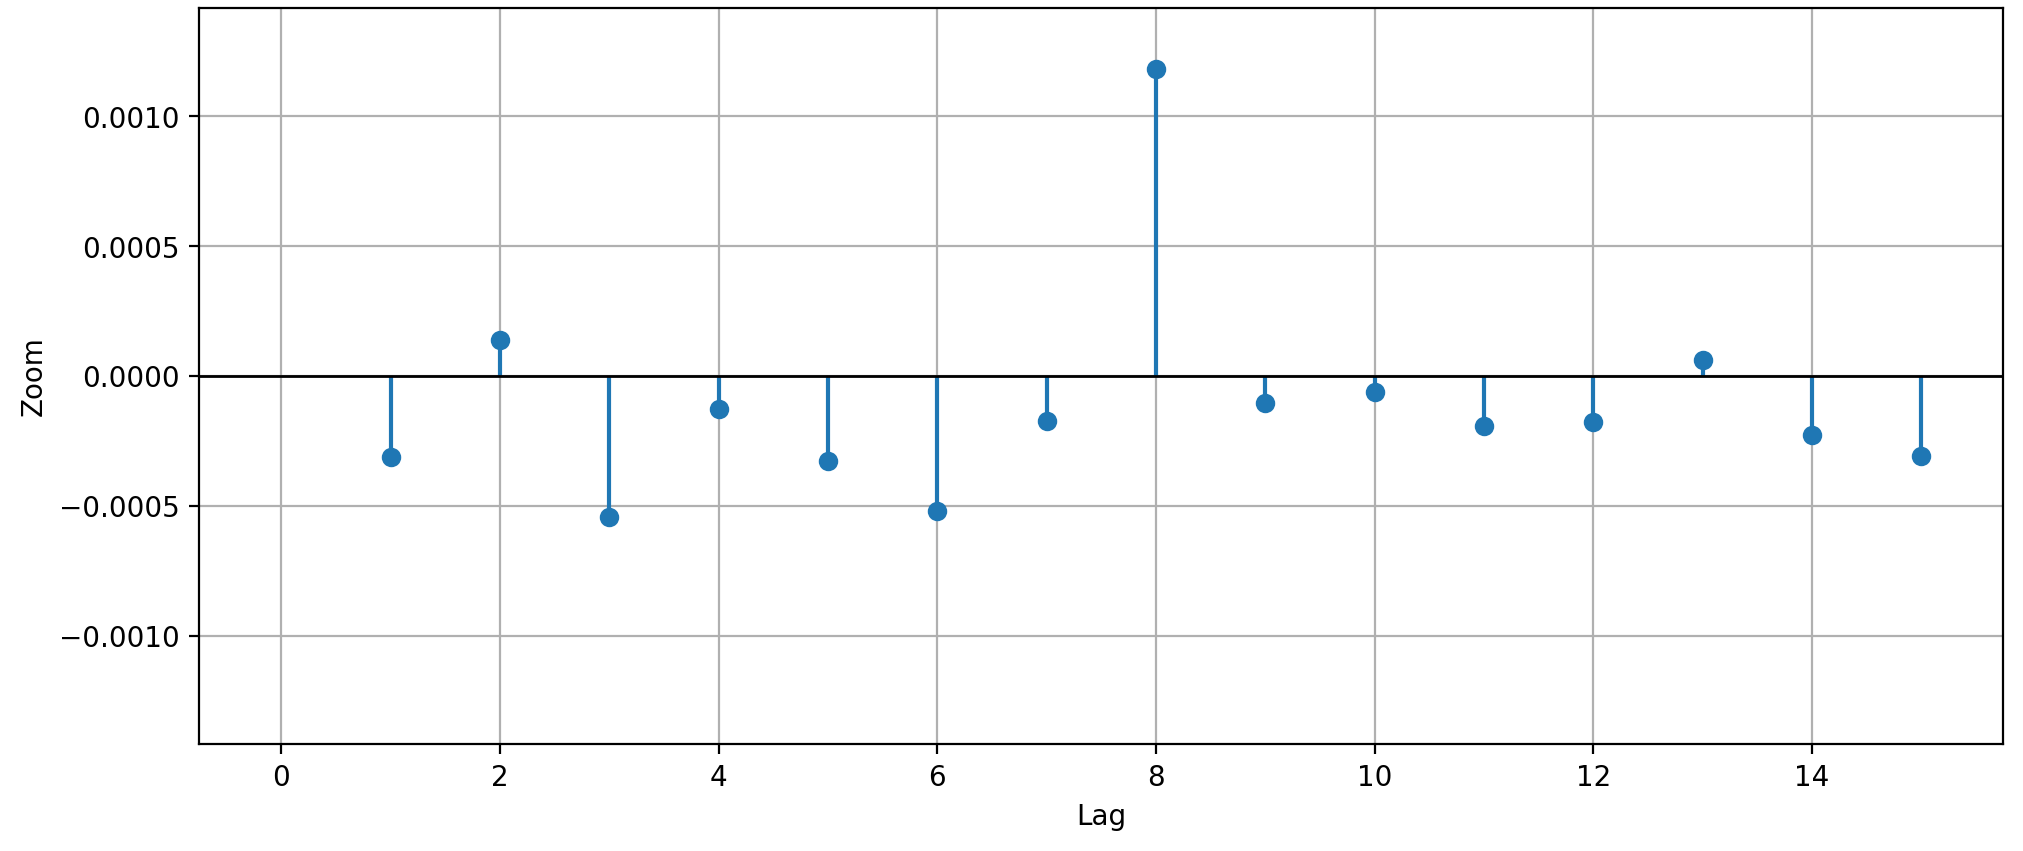
\includegraphics[width=0.9\textwidth]{gfx/no_wh_ac.png}
    \caption{Autokorelacja badanego strumienia bitów dla opóźnień od 0 do 15}
    \label{fig:autokorelacja_bitstream}
\end{figure}

\begin{table}[htbp]
    \centering
    \caption{Wartości współczynników autokorelacji dla badanego strumienia bitów}
    \label{tab:autokorelacja_wyniki}
    \small
    \begin{tabular}{rrrr}
        \toprule
        Opóźnienie & $R$ & Opóźnienie & $R$ \\
        \midrule
        0 & $+1{,}000000$ & 8  & $+0{,}001182$ \\
        1 & $-0{,}000309$ & 9  & $-0{,}000102$ \\
        2 & $+0{,}000139$ & 10 & $-0{,}000060$ \\
        3 & $-0{,}000544$ & 11 & $-0{,}000192$ \\
        4 & $-0{,}000127$ & 12 & $-0{,}000176$ \\
        5 & $-0{,}000326$ & 13 & $+0{,}000061$ \\
        6 & $-0{,}000520$ & 14 & $-0{,}000226$ \\
        7 & $-0{,}000173$ & 15 & $-0{,}000306$ \\
        \bottomrule
    \end{tabular}
\end{table}

Na podstawie otrzymanych wyników można stwierdzić, że poza oczywistą wartością równą
jedności dla opóźnienia zerowego wszystkie współczynniki autokorelacji pozostają bliskie
zeru, nie przekraczając wartości bezwzględnej $1{,}2 \cdot 10^{-3}$. W badanym zakresie nie
zaobserwowano narastającego trendu ani wartości sugerujących silną zależność pomiędzy
kolejnymi bitami.

Interpretacja tych wielkości wymaga jednak odniesienia do rozrzutu statystycznego. Dla
strumienia w pełni losowego o długości $N$ bitów wyznaczone współczynniki wahają się wokół
zera z odchyleniem standardowym w przybliżeniu równym $1/\sqrt{N}$, co dla badanej serii
daje wartość $\sigma \approx 3{,}1 \cdot 10^{-4}$. Zdecydowana większość odnotowanych
wartości nie przekracza dwukrotności tego poziomu i mieści się w granicach naturalnych
fluktuacji.

Wyjątkiem jest opóźnienie równe 8, dla którego uzyskano $R = 0{,}001182$, czyli blisko
czterokrotność odchylenia standardowego. Wartość ta odstaje od pozostałych, a jej położenie
nie jest przypadkowe, ponieważ opóźnienie 8 odpowiada zarówno liczbie oscylatorów
pierścieniowych, jak i długości bajtu wystawianego przez moduł ekstrakcji entropii. Bity
zapisywane są do bufora w stałej kolejności numerów kanałów, wobec czego pozycje odległe
o osiem miejsc pochodzą statystycznie częściej z tego samego oscylatora niż pozycje
sąsiednie. Zaobserwowane odchylenie należy zatem wiązać z deterministyczną strukturą
serializacji, a nie z ogólnym brakiem losowości źródła. Pozostałe opóźnienia będące
wielokrotnościami ośmiu nie wykazują podobnego wzmocnienia, co wskazuje, że efekt ma
charakter lokalny i nie prowadzi do wystąpienia periodyczności w dłuższej skali.

Analiza autokorelacji została potraktowana jako test kontrolny, pozwalający wychwycić
problemy implementacyjne jeszcze przed wykonaniem bardziej rozbudowanych badań
statystycznych. W przypadku projektów sprzętowych takie podejście jest szczególnie
przydatne, ponieważ umożliwia szybkie porównanie wyników po każdej zmianie konfiguracji
układu FPGA. Uzyskany wynik nie wskazuje na błąd implementacji, wyznacza natomiast
kierunek dalszej analizy, którą przedstawiono w kolejnych podrozdziałach dotyczących
strumienia poddanego wybielaniu oraz dwuwymiarowych map opóźnień.

\FloatBarrier

\subsection{Wyniki pomiaru dla 8 oscylatorów rozproszonych w strukturze układu}

W poprzedniej konfiguracji oscylatory zostały rozmieszczone automatycznie, bez narzucenia
ograniczeń położenia, w efekcie czego narzędzie implementacyjne umieściło je w zwartym
obszarze struktury. Takie sąsiedztwo jest niekorzystne z punktu widzenia jakości źródła
entropii, ponieważ oscylatory położone blisko siebie pracują w niemal identycznych
warunkach temperaturowych i zasilania, a dodatkowo pozostają podatne na wzajemne
oddziaływanie poprzez sprzężenia pojemnościowe i wspólną sieć dystrybucji zasilania.
Zjawiska te mogą prowadzić do częściowej synchronizacji przebiegów, co obniża efektywną
liczbę niezależnych źródeł szumu poniżej liczby zaimplementowanych oscylatorów.
Rozproszenie struktur w obrębie układu ma na celu ograniczenie tych zależności oraz
zróżnicowanie lokalnych warunków pracy poszczególnych pierścieni.

Przebieg współczynnika autokorelacji dla konfiguracji z oscylatorami rozproszonymi
przedstawiono na rysunku~\ref{fig:autokorelacja_rozproszone}, natomiast dokładne wartości
liczbowe zestawiono w tabeli~\ref{tab:autokorelacja_rozproszone}.

\begin{figure}[htbp]
    \centering
    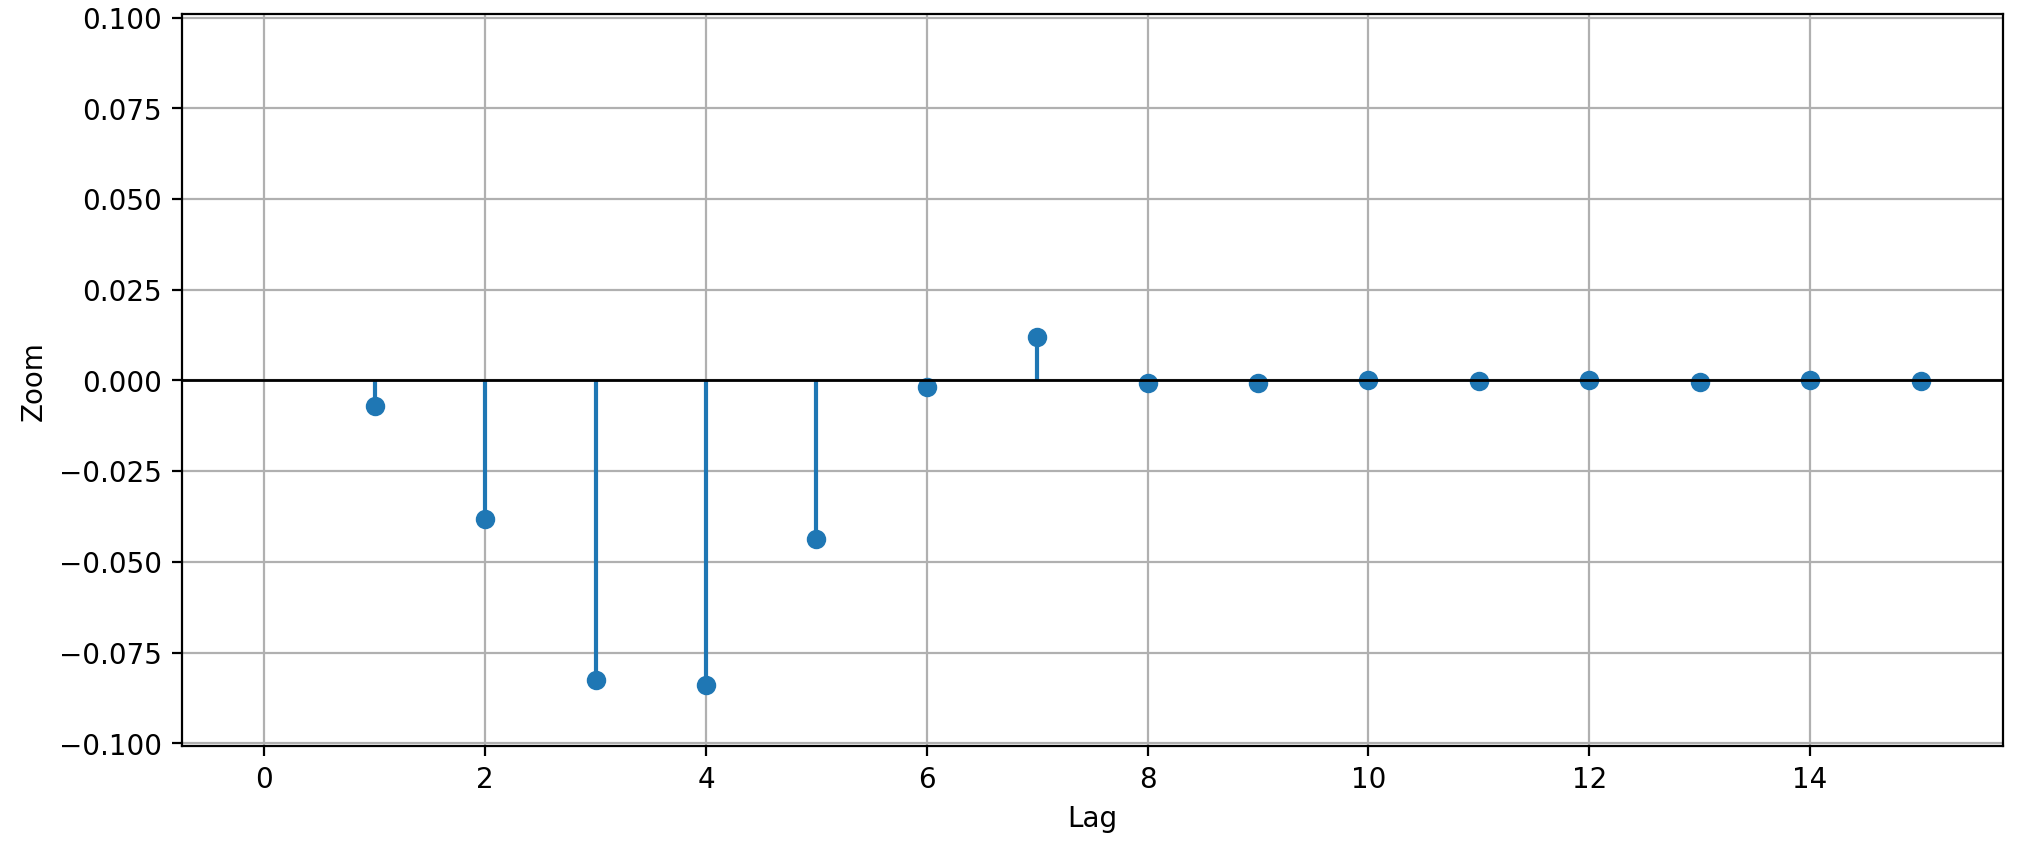
\includegraphics[width=0.9\textwidth]{gfx/spread_ac.png}
    \caption{Autokorelacja strumienia bitów dla oscylatorów rozproszonych w strukturze
    układu, opóźnienia od 0 do 15}
    \label{fig:autokorelacja_rozproszone}
\end{figure}

\begin{table}[htbp]
    \centering
    \caption{Wartości współczynników autokorelacji dla oscylatorów rozproszonych
    w strukturze układu}
    \label{tab:autokorelacja_rozproszone}
    \small
    \begin{tabular}{rrrr}
        \toprule
        Opóźnienie & $R$ & Opóźnienie & $R$ \\
        \midrule
        0 & $+1{,}000000$ & 8  & $-0{,}000588$ \\
        1 & $-0{,}007122$ & 9  & $-0{,}000635$ \\
        2 & $-0{,}038163$ & 10 & $+0{,}000056$ \\
        3 & $-0{,}082474$ & 11 & $-0{,}000165$ \\
        4 & $-0{,}084080$ & 12 & $+0{,}000065$ \\
        5 & $-0{,}043632$ & 13 & $-0{,}000489$ \\
        6 & $-0{,}001822$ & 14 & $+0{,}000223$ \\
        7 & $+0{,}011959$ & 15 & $-0{,}000210$ \\
        \bottomrule
    \end{tabular}
\end{table}

Uzyskany wynik różni się zasadniczo od poprzedniego. W zakresie opóźnień od 1 do 5
występują wyraźnie ujemne współczynniki autokorelacji, osiągające wartość
$-0{,}084080$ dla opóźnienia równego 4. Przy długości serii $N = 10\,485\,760$ bitów
odchylenie standardowe współczynnika dla strumienia w pełni losowego wynosi
$\sigma \approx 3{,}1 \cdot 10^{-4}$, wobec czego zaobserwowana wartość odpowiada
około 270-krotności tego poziomu. Jest to zależność jednoznacznie istotna statystycznie,
a nie efekt naturalnych fluktuacji. Warto zaznaczyć, że wykryte odchylenia mają znak
ujemny, przez co nie mogą być wyjaśnione ewentualną nierównowagą liczby zer i jedynek,
gdyż niezerowa wartość średnia strumienia przesuwałaby współczynniki w kierunku wartości
dodatnich.

Charakter zaobserwowanej zależności wskazuje na skłonność strumienia do naprzemiennej
zmiany wartości bitów w krótkiej skali. Współczynniki narastają w wartości bezwzględnej
od opóźnienia 1 do 4, po czym maleją, a dla opóźnienia 7 przyjmują wartość dodatnią
$+0{,}011959$, co odpowiada blisko 40-krotności odchylenia standardowego. Taki przebieg,
złożony z ujemnego obszaru zakończonego dodatnim maksimum, jest typowy dla strumienia
o częściowo okresowej strukturze, w którym kolejne bity nie są generowane niezależnie,
lecz w powtarzalnym porządku wynikającym z pracy układu ekstrakcji. Ponieważ bity
zapisywane są do bufora w stałej kolejności numerów kanałów, a dla pojedynczego
oscylatora zbocza narastające i opadające występują naprzemiennie, uporządkowanie
oscylatorów według częstotliwości pracy przekłada się bezpośrednio na uporządkowanie
wartości w strumieniu wyjściowym. Zależność ta ma zatem źródło w warstwie serializacji
oraz w relacjach częstotliwości pomiędzy poszczególnymi pierścieniami, a nie w samym
rozproszeniu struktur w obrębie układu.

Dla opóźnień od 8 do 15 wartości współczynników nie przekraczają dwukrotności odchylenia
standardowego i pozostają w granicach naturalnych fluktuacji, co oznacza, że wykryta
zależność ma zasięg ograniczony do kilku najbliższych pozycji i nie prowadzi do
periodyczności w dłuższej skali. Nie odnotowano również wzmocnienia dla opóźnienia
równego 8, obecnego w poprzedniej konfiguracji, co potwierdza, że zmiana rozmieszczenia
oscylatorów wpłynęła na strukturę strumienia, jednak przesunęła obserwowane zależności
w obszar mniejszych opóźnień, zamiast je usunąć.

Wynik ten należy uznać za istotny z punktu widzenia dalszych badań. Pokazuje on, że
poprawa warunków pracy samych źródeł entropii nie jest wystarczająca, jeżeli sposób
łączenia bitów pochodzących z wielu kanałów wprowadza własną, deterministyczną strukturę.
Uzasadnia to konieczność zastosowania etapu korekcji strumienia, którego skuteczność
zbadano w kolejnym podrozdziale, oraz analizy dwuwymiarowych map opóźnień, pozwalającej
ocenić, czy wykryta zależność obejmuje również poziom całych słów.

\FloatBarrier

\subsection{Wyniki pomiaru dla 16 oscylatorów łączonych parami operacją XOR}

W kolejnej konfiguracji liczbę oscylatorów pierścieniowych zwiększono do szesnastu,
przy czym ich wyjścia łączone są parami operacją różnicy symetrycznej, w wyniku czego
do modułu ekstrakcji trafia nadal osiem sygnałów, a przepustowość generatora pozostaje
niezmieniona. Rozmieszczenie struktur w obrębie układu ustalono ręcznie, tak aby
oscylatory tworzące jedną parę znajdowały się w odległych obszarach logiki.

Zastosowanie operacji XOR do łączenia wyjść ma dwie zasadnicze zalety. Po pierwsze,
odchylenie prawdopodobieństwa sygnału wynikowego jest iloczynem odchyleń sygnałów
wejściowych, wobec czego połączenie dwóch niedoskonałych źródeł daje sygnał o rozkładzie
bliższym równomiernemu niż każde z nich osobno. Po drugie, przewidzenie wartości sygnału
wynikowego wymaga znajomości stanu obu oscylatorów jednocześnie, co ogranicza wpływ
okresowego zachowania pojedynczego pierścienia na strumień wyjściowy. Rozdzielenie
przestrzenne oscylatorów tworzących parę jest przy tym warunkiem skuteczności tego
rozwiązania, ponieważ w przypadku struktur położonych blisko siebie wzajemne
oddziaływanie mogłoby prowadzić do ich częściowej synchronizacji, a operacja XOR na dwóch
skorelowanych sygnałach nie wnosi dodatkowej entropii.

Przebieg współczynnika autokorelacji dla omawianej konfiguracji przedstawiono na
rysunku~\ref{fig:autokorelacja_xor}, natomiast dokładne wartości liczbowe zestawiono
w tabeli~\ref{tab:autokorelacja_xor}.

\begin{figure}[htbp]
    \centering
    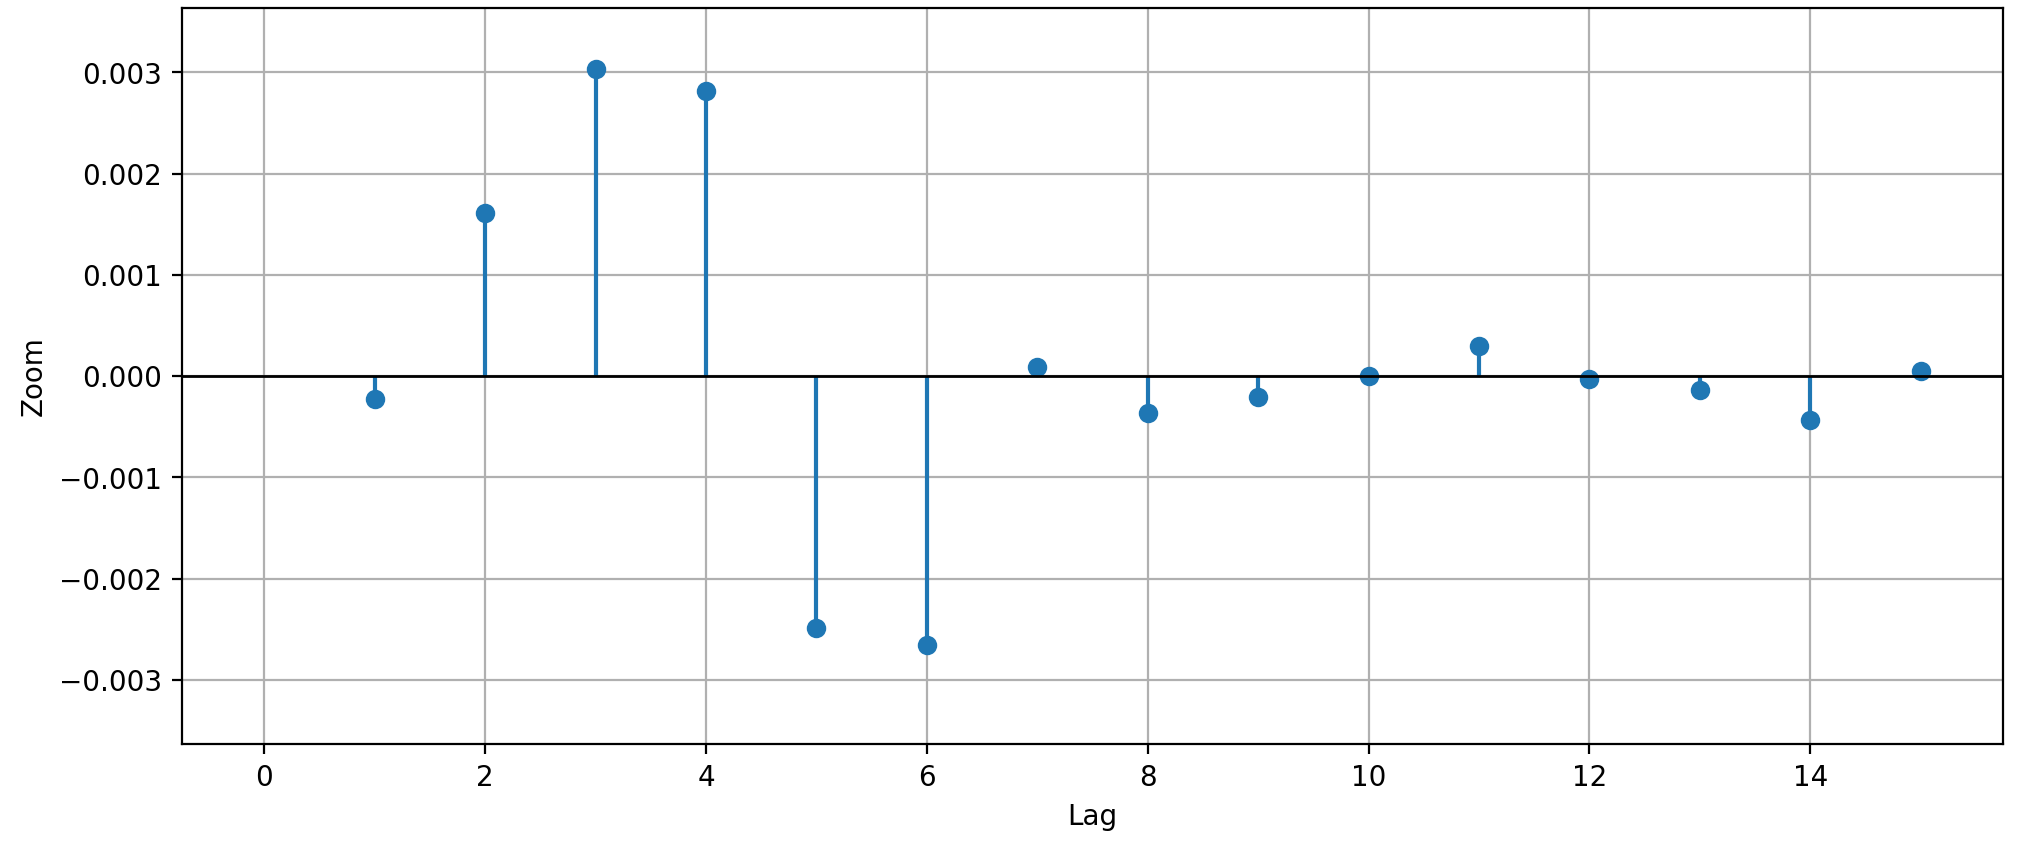
\includegraphics[width=0.9\textwidth]{gfx/xor_ac.png}
    \caption{Autokorelacja strumienia bitów dla 16 oscylatorów łączonych parami operacją
    XOR, opóźnienia od 0 do 15. Zakres dolnego wykresu wynosi $\pm 3 \cdot 10^{-3}$}
    \label{fig:autokorelacja_xor}
\end{figure}

\begin{table}[htbp]
    \centering
    \caption{Wartości współczynników autokorelacji dla 16 oscylatorów łączonych parami
    operacją XOR}
    \label{tab:autokorelacja_xor}
    \small
    \begin{tabular}{rrrr}
        \toprule
        Opóźnienie & $R$ & Opóźnienie & $R$ \\
        \midrule
        0 & $+1{,}000000$ & 8  & $-0{,}000359$ \\
        1 & $-0{,}000221$ & 9  & $-0{,}000207$ \\
        2 & $+0{,}001612$ & 10 & $-0{,}000004$ \\
        3 & $+0{,}003030$ & 11 & $+0{,}000297$ \\
        4 & $+0{,}002819$ & 12 & $-0{,}000024$ \\
        5 & $-0{,}002487$ & 13 & $-0{,}000133$ \\
        6 & $-0{,}002656$ & 14 & $-0{,}000437$ \\
        7 & $+0{,}000093$ & 15 & $+0{,}000047$ \\
        \bottomrule
    \end{tabular}
\end{table}

Zmiana konfiguracji przyniosła wyraźną poprawę w stosunku do poprzedniego pomiaru.
Największa wartość bezwzględna współczynnika dla opóźnień większych od zera wynosi
$0{,}003030$ i występuje dla opóźnienia równego 3, podczas gdy w konfiguracji bez
łączenia wyjść operacją XOR wartość skrajna sięgała $0{,}084080$. Amplituda
zaobserwowanych zależności zmalała zatem blisko dwudziestoośmiokrotnie. Należy przy tym
zwrócić uwagę, że zakres pionowej osi dolnego wykresu na
rysunku~\ref{fig:autokorelacja_xor} jest dobierany automatycznie do zakresu danych
i wynosi w tym przypadku około $\pm 3 \cdot 10^{-3}$, wobec czego bezpośrednie porównanie
wizualne obu rysunków bez uwzględnienia podziałki prowadziłoby do błędnych wniosków.

Wykryte odchylenia pozostają jednak istotne statystycznie. Przy odchyleniu standardowym
$\sigma \approx 3{,}1 \cdot 10^{-4}$ współczynniki dla opóźnień od 2 do 6 odpowiadają
wielokrotnościom tego poziomu w zakresie od pięciu do niemal dziesięciu, co wyklucza
wyjaśnienie ich jako naturalnych fluktuacji. Zmienił się natomiast charakter zależności.
W poprzedniej konfiguracji wszystkie współczynniki w zakresie małych opóźnień były
ujemne, co odpowiadało skłonności do naprzemiennej zmiany wartości bitów. Obecnie
występuje wyraźny podział: dla opóźnień od 2 do 4 współczynniki są dodatnie, natomiast
dla opóźnień 5 i 6 ujemne, przy praktycznym zaniku zależności dla opóźnienia 7
i wszystkich większych. Taki przebieg, obejmujący zwarty obszar zależności dodatnich
przechodzących w ujemne, wskazuje na obecność składowej o okresie rzędu ośmiu pozycji
w strumieniu wyjściowym, a więc odpowiadającej długości pojedynczego bajtu i liczbie
kanałów doprowadzonych do modułu ekstrakcji.

Obserwacja ta potwierdza wniosek sformułowany w poprzednim podrozdziale, zgodnie z którym
zasadnicza część wykrywanych zależności ma źródło w warstwie łączenia bitów pochodzących
z wielu kanałów, a nie w jakości samych źródeł entropii. Podwojenie liczby oscylatorów
oraz łączenie ich wyjść operacją XOR poprawiło właściwości poszczególnych sygnałów
wejściowych, co przełożyło się na znaczną redukcję amplitudy zależności, nie usunęło
jednak deterministycznej struktury wynikającej ze stałej kolejności zapisu kanałów do
bufora. Całkowite wyeliminowanie tego efektu wymagałoby modyfikacji sposobu serializacji
lub zastosowania korekcji strumienia, której skuteczność zbadano w kolejnym podrozdziale.

\FloatBarrier

\subsection{Wyniki pomiaru dla 16 oscylatorów z wybielaniem metodą von Neumanna}

Ostatnia z badanych konfiguracji opiera się na tej samej implementacji sprzętowej co
poprzednia, obejmującej szesnaście oscylatorów pierścieniowych łączonych parami operacją
XOR i rozmieszczonych ręcznie w oddalonych obszarach struktury układu. Różnica dotyczy
wyłącznie przetwarzania po stronie komputera: zarejestrowany strumień poddano wybielaniu
metodą von Neumanna przed wyznaczeniem współczynników autokorelacji.

Analiza tej samej serii pomiarowej w postaci surowej oraz wybielonej pozwala rozdzielić
dwa rodzaje odstępstw od losowości. Metoda von Neumanna usuwa odchylenie
prawdopodobieństwa wystąpienia zera i jedynki, jest natomiast skuteczna wyłącznie przy
założeniu wzajemnej niezależności kolejnych bitów strumienia wejściowego. Odrzucenie par
o jednakowych wartościach zmienia dodatkowo długość i uporządkowanie strumienia, wobec
czego opóźnienia po wybielaniu nie odpowiadają bezpośrednio pozycjom w strumieniu surowym,
a wynikające z tego przesunięcie należy uwzględnić przy porównywaniu obu przebiegów.

Przebieg współczynnika autokorelacji dla strumienia wybielonego przedstawiono na
rysunku~\ref{fig:autokorelacja_vn}, natomiast dokładne wartości liczbowe zestawiono
w tabeli~\ref{tab:autokorelacja_vn}.

\begin{figure}[htbp]
    \centering
    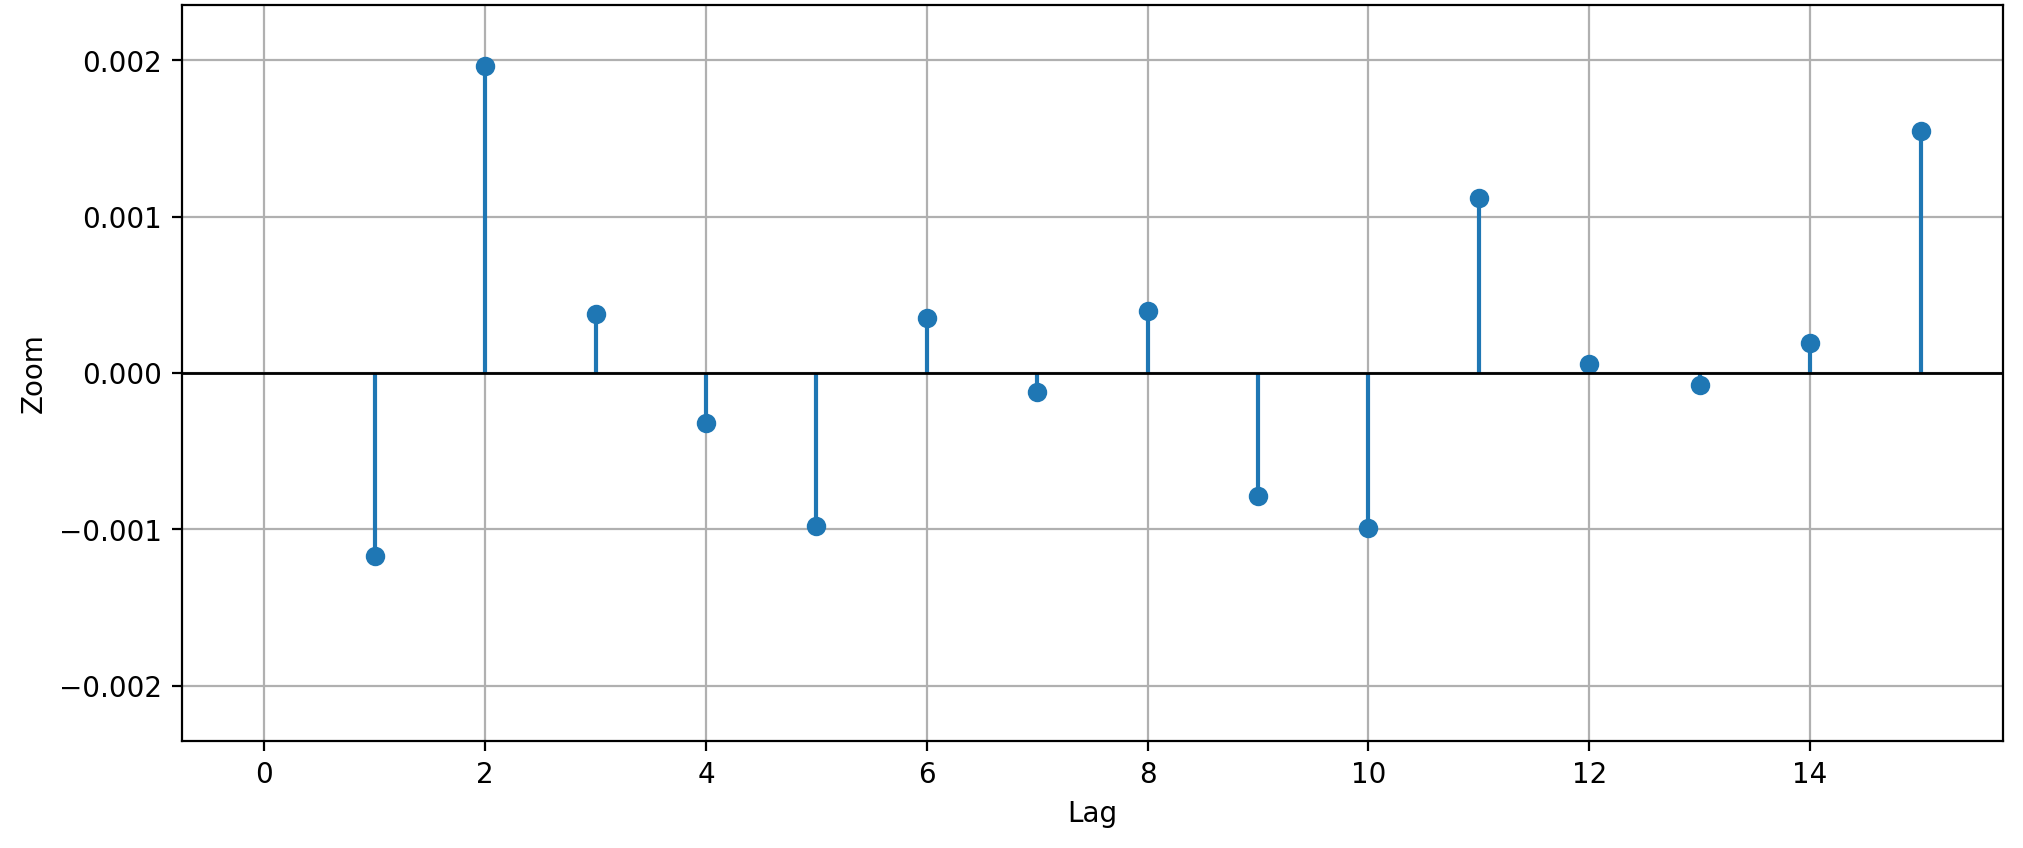
\includegraphics[width=0.9\textwidth]{gfx/vn_ac.png}
    \caption{Autokorelacja strumienia bitów dla 16 oscylatorów łączonych parami operacją
    XOR, po wybielaniu metodą von Neumanna, opóźnienia od 0 do 15. Zakres dolnego wykresu
    wynosi około $\pm 2 \cdot 10^{-3}$}
    \label{fig:autokorelacja_vn}
\end{figure}

\begin{table}[htbp]
    \centering
    \caption{Wartości współczynników autokorelacji dla 16 oscylatorów łączonych parami
    operacją XOR, po wybielaniu metodą von Neumanna}
    \label{tab:autokorelacja_vn}
    \small
    \begin{tabular}{rrrr}
        \toprule
        Opóźnienie & $R$ & Opóźnienie & $R$ \\
        \midrule
        0 & $+1{,}000000$ & 8  & $+0{,}000395$ \\
        1 & $-0{,}001172$ & 9  & $-0{,}000784$ \\
        2 & $+0{,}001963$ & 10 & $-0{,}000990$ \\
        3 & $+0{,}000378$ & 11 & $+0{,}001122$ \\
        4 & $-0{,}000321$ & 12 & $+0{,}000056$ \\
        5 & $-0{,}000977$ & 13 & $-0{,}000079$ \\
        6 & $+0{,}000352$ & 14 & $+0{,}000193$ \\
        7 & $-0{,}000122$ & 15 & $+0{,}001549$ \\
        \bottomrule
    \end{tabular}
\end{table}

Strumień po wybielaniu liczy $2\,620\,032$ bitów, co odpowiada $24{,}99\%$ długości
strumienia wejściowego. Wartość ta jest praktycznie równa teoretycznej granicy jednej
czwartej, osiąganej przez metodę von Neumanna dla źródła o rozkładzie równomiernym.
Sama wydajność wybielania stanowi zatem niezależne potwierdzenie, że strumień wejściowy
nie wykazywał istotnego odchylenia liczby zer i jedynek, ponieważ każde takie odchylenie
prowadziłoby do zwiększenia udziału par odrzucanych i wyraźnie mniejszej długości
wyniku.

Skrócenie serii wymaga skorygowania progu istotności statystycznej. Dla omawianego
strumienia odchylenie standardowe współczynnika autokorelacji przy założeniu pełnej
losowości wynosi $\sigma \approx 6{,}2 \cdot 10^{-4}$, a więc dwukrotnie więcej niż
w poprzednich pomiarach, w których analizowano serie o pełnej długości. Bezpośrednie
porównywanie wartości liczbowych z wcześniejszymi tabelami bez uwzględnienia tej różnicy
byłoby nieuprawnione.

Największą wartość bezwzględną odnotowano dla opóźnienia równego 2, gdzie uzyskano
$R = 0{,}001963$, co odpowiada około 3,2-krotności odchylenia standardowego. Przy
piętnastu jednocześnie badanych opóźnieniach oczekiwana wartość maksymalna dla źródła
losowego mieści się w okolicach trzech odchyleń standardowych, wobec czego zaobserwowany
wynik znajduje się na granicy istotności i nie stanowi sam w sobie dowodu obecności
zależności. Pozostałe współczynniki, w tym $+0{,}001549$ dla opóźnienia 15 oraz
$-0{,}001172$ dla opóźnienia 1, nie przekraczają dwóch i pół odchylenia standardowego.

Istotną zmianą w stosunku do strumienia surowego jest zniknięcie uporządkowanej struktury
obejmującej opóźnienia od 2 do 6. W pomiarze bez wybielania współczynniki w tym zakresie
tworzyły zwarty obszar wartości dodatnich przechodzących w ujemne, przy czym każda z nich
przekraczała pięciokrotność odchylenia standardowego. Po wybielaniu znaki współczynników
w całym badanym zakresie rozkładają się nieregularnie, a ich wartości nie tworzą
rozpoznawalnego wzorca, co odpowiada obrazowi oczekiwanemu dla strumienia bez zależności
lokalnych. Należy przy tym pamiętać, że odrzucanie par o jednakowych wartościach
przekształca skalę opóźnień, wobec czego zależność występująca w strumieniu surowym na
określonej pozycji nie zostałaby po wybielaniu odwzorowana na tej samej pozycji, lecz
rozmyta w otoczeniu proporcjonalnym do stopnia redukcji długości. Sam brak struktury
w przebiegu po wybielaniu nie jest zatem równoważny stwierdzeniu, że mechanizm
odpowiedzialny za jej powstanie przestał działać w warstwie sprzętowej.

Zestawienie wyników wszystkich czterech badanych konfiguracji, wraz z odniesieniem do
pozostałych zastosowanych metod analizy statystycznej, przedstawiono w~podrozdziale
podsumowującym.

\FloatBarrier

\section{Analiza utworzonych słów bitowych za pomocą map 2D}

Mapy dwuwymiarowe zastosowano w celu oceny właściwości statystycznych słów utworzonych z badanego 
strumienia bitów oraz analizy zależności pomiędzy słowami oddalonymi od siebie o zadane opóźnienie. 
Dla każdej rozpatrywanej konfiguracji wyznaczano pary w postaci $(w[n],\,w[n+\tau])$, gdzie $w[n]$ 
oznacza bieżące słowo bitowe, natomiast $w[n+\tau]$ słowo przesunięte o opóźnienie $\tau$. 
Następnie ilość wystąpień poszczególnych par przedstawiano w postaci histogramu dwuwymiarowego.

W przypadku generatora o dobrych właściwościach losowych rozkład punktów na mapie 2D powinien być 
możliwie jednorodny, bez wyraźnych struktur geometrycznych, pasów oraz nadmiernej koncentracji 
zliczeń w określonych obszarach. 
Pojawienie się pasów pionowych lub poziomych wskazuje, że niektóre wartości słów występują 
częściej od innych, co świadczy o nierównomierności rozkładu. 
Z kolei zwiększona koncentracja punktów w pobliżu przekątnej może sugerować istnienie zależności 
pomiędzy kolejnymi słowami, a więc obecność korelacji czasowej w analizowanym ciągu.

\FloatBarrier

\subsection{Mapy dla 8 oscylatorów rozmieszczonych automatycznie}

Analizę map dwuwymiarowych rozpoczęto od konfiguracji podstawowej, w~której oscylatory
zostały rozmieszczone automatycznie przez narzędzie implementacyjne. Mapy dla słów
czterobitowych przedstawiono na rysunku~\ref{fig:map2d_auto_w4}.

\begin{figure}[ht]
    \centering
    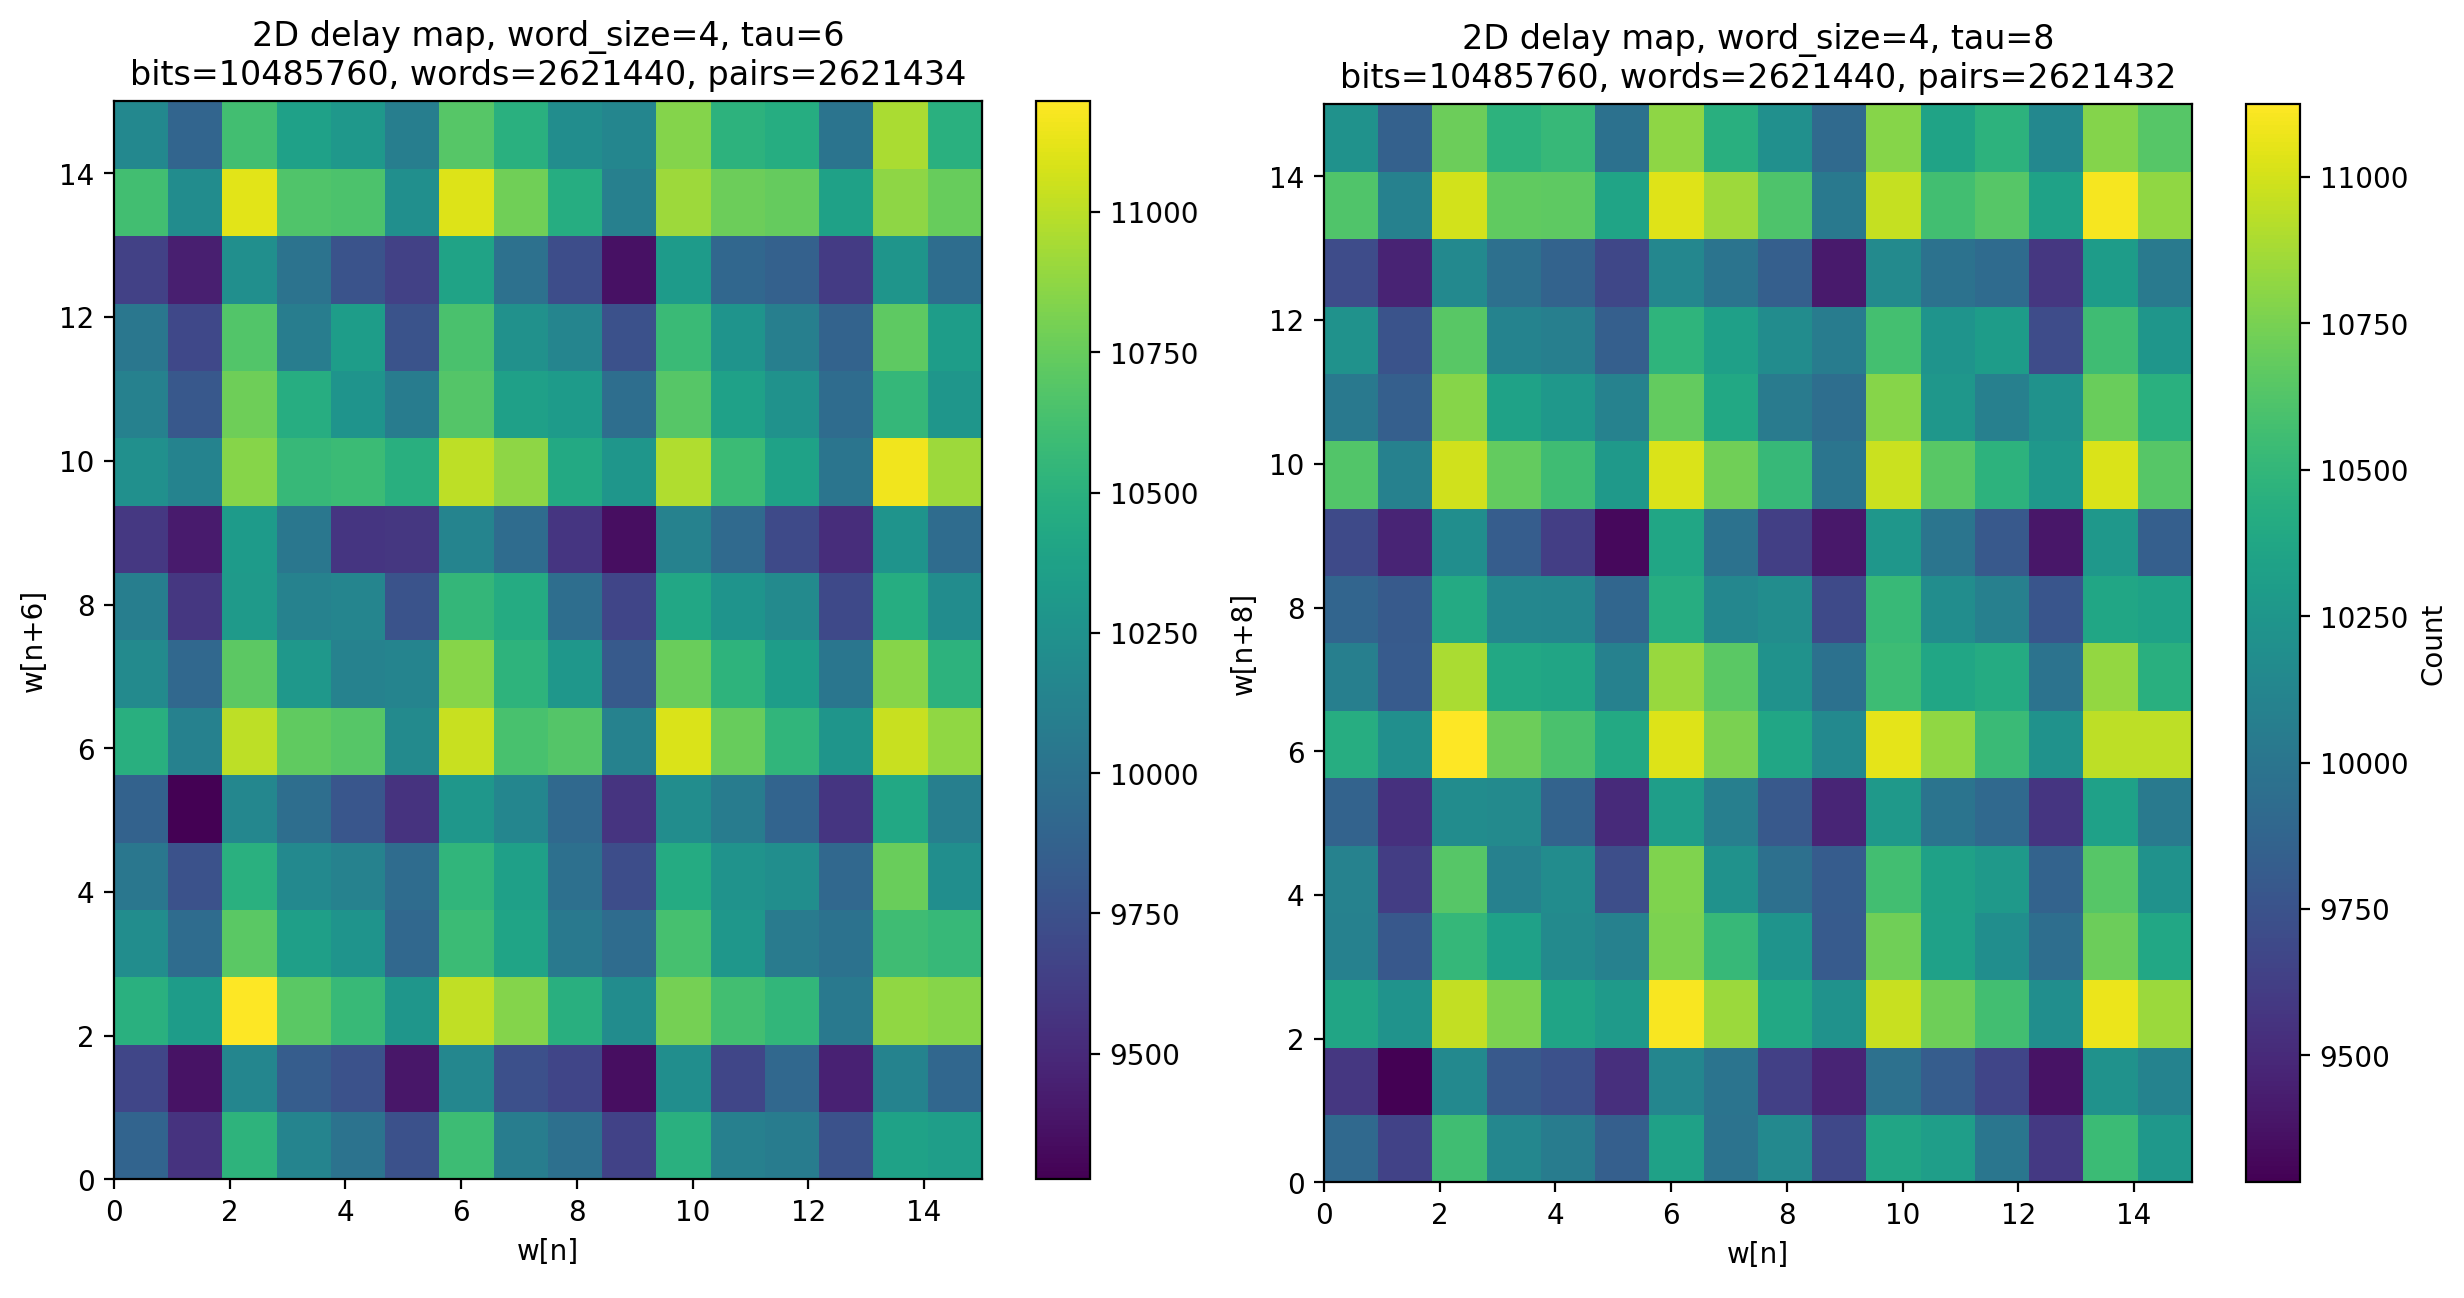
\includegraphics[width=0.98\textwidth]{gfx/no_wh_2d_w4_t6_t8}
    \caption{Mapy 2D dla 8 oscylatorów rozmieszczonych automatycznie, przy parametrach
    $word\_size = 4$ oraz $\tau = 6$, $\tau = 8$.}
    \label{fig:map2d_auto_w4}
\end{figure}

Dla słów czterobitowych widoczny jest regularny układ jaśniejszych i~ciemniejszych pasów,
biegnących zarówno poziomo, jak i~pionowo. Podwyższone zliczenia występują dla wartości
słów o~numerach $2$, $6$, $10$ oraz $14$, natomiast obniżone dla wartości $1$, $5$, $9$
i~$13$. Wszystkie wyróżnione wartości mają wspólną cechę: różnią się o~cztery, a~więc
odpowiadają jednakowemu stanowi dwóch najmłodszych bitów przy zmiennych bitach starszych.
Wskazuje to, że nierównomierność dotyczy przede wszystkim określonych pozycji w~obrębie
słowa, a~zatem konkretnych kanałów wejściowych, nie zaś wartości słowa jako całości.

Przy $2\,621\,434$ analizowanych parach i~$256$ komórkach histogramu wartość oczekiwana
zliczenia wynosi $10\,240$, a~odpowiadające jej odchylenie standardowe rozkładu Poissona
około $101$ zliczeń. Odnotowany zakres, obejmujący przedział od około $9\,400$ do
$11\,100$, odpowiada zatem odchyleniu skrajnemu na poziomie $8{,}5$ odchylenia
standardowego. Rozkład wartości słów odbiega więc od równomiernego w~sposób jednoznacznie
istotny statystycznie, choć skala tego odstępstwa jest znacznie mniejsza niż stwierdzona
później dla konfiguracji z~ręcznym rozmieszczeniem oscylatorów.

Struktura pasowa jest praktycznie identyczna dla obu badanych opóźnień, co oznacza, że
wynika ona z~rozkładu prawdopodobieństwa pojedynczych słów, a~nie z~zależności pomiędzy
słowami oddalonymi w~strumieniu. Mapa dwuwymiarowa jest w~tym przypadku w~przybliżeniu
iloczynem dwóch identycznych rozkładów brzegowych, co odpowiada wzajemnej niezależności
obu współrzędnych przy jednoczesnym odstępstwie każdej z~nich od rozkładu równomiernego.
Nie zaobserwowano również podwyższonych zliczeń wzdłuż przekątnej, a~więc powtarzalność
całych słów po zadanym opóźnieniu nie występuje.

\begin{figure}[ht]
    \centering
    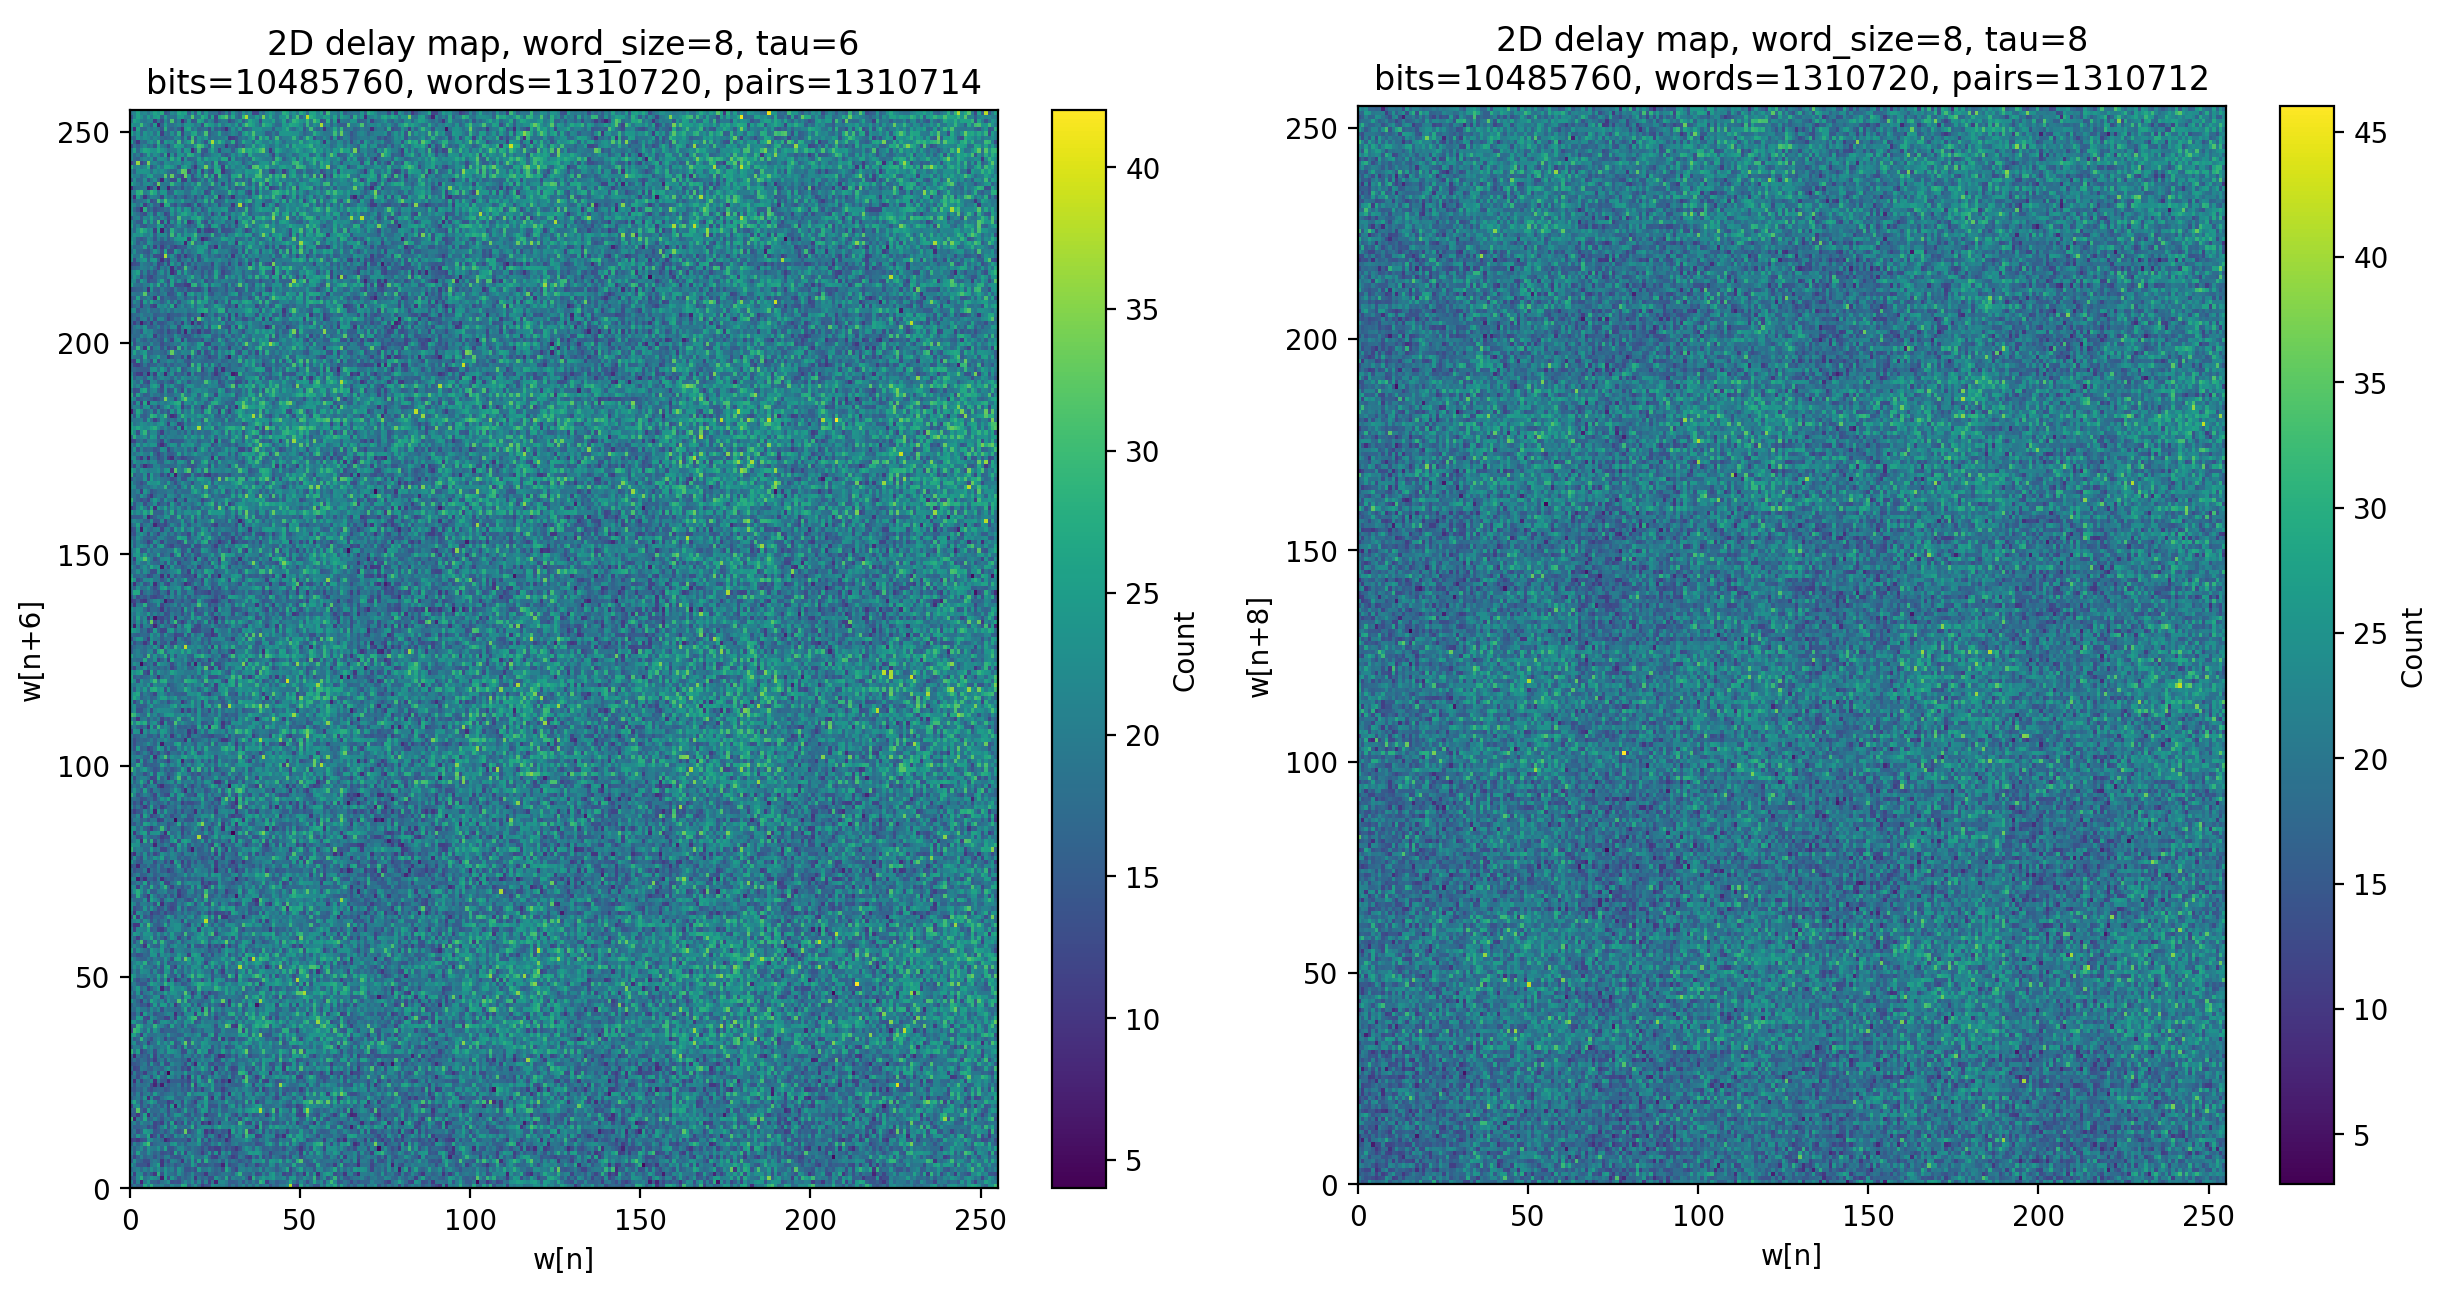
\includegraphics[width=0.98\textwidth]{gfx/no_wh_2d_w8_t6_t8}
    \caption{Mapy 2D dla 8 oscylatorów rozmieszczonych automatycznie, przy parametrach
    $word\_size = 8$ oraz $\tau = 6$, $\tau = 8$.}
    \label{fig:map2d_auto_w8}
\end{figure}

Mapy dla słów ośmiobitowych, przedstawione na rysunku~\ref{fig:map2d_auto_w8}, mają
charakter drobnoziarnistego szumu, w~którym regularna struktura widoczna dla słów
czterobitowych przestaje być rozpoznawalna. Wynika to z~liczności: przy $1\,310\,714$
parach rozłożonych na $65\,536$ komórek wartość oczekiwana zliczenia wynosi zaledwie
dwadzieścia, a~odpowiadające jej odchylenie standardowe około cztery i~pół. Odnotowany
zakres od trzech do czterdziestu sześciu zliczeń odpowiada odchyleniu skrajnemu rzędu
pięciu do sześciu odchyleń standardowych, jednak przy tak dużej liczbie komórek
rozpatrywanych jednocześnie wystąpienie takich wartości jest oczekiwane dla źródła
losowego. Mapa ta potwierdza zatem jedynie brak struktur wielkoskalowych i~nie pozwala
na ilościową ocenę rozkładu, a~za miarodajne dla tej konfiguracji przyjęto wyniki
uzyskane dla słów czterobitowych.

Zestawienie tego wyniku z~testem odchylenia rozkładu prowadzi do obserwacji wartej
podkreślenia. Dla omawianej konfiguracji test monobitowy wykazał odchylenie na poziomie
jedenastu odchyleń standardowych, a~mapy dwuwymiarowe rozrzut zliczeń na poziomie
ośmiu i~pół. Obie metody wskazują zatem zgodnie na istotne odstępstwo od losowości,
przy czym mapy dodatkowo lokalizują je: nierównomierność dotyczy wybranych pozycji
bitowych w~obrębie słowa, co odpowiada zróżnicowaniu właściwości poszczególnych
kanałów wejściowych, a~nie jednolitemu przesunięciu całego strumienia.

\FloatBarrier

\subsection{Mapy dla 8 oscylatorów rozproszonych w strukturze układu}

W konfiguracji z oscylatorami rozmieszczonymi ręcznie w oddalonych obszarach struktury
mapy dwuwymiarowe zachowują ogólny charakter obrazu uzyskanego poprzednio, ujawniają
jednak wyraźniejszą strukturę wewnętrzną. Mapy dla słów czterobitowych przedstawiono na
rysunku~\ref{fig:map2d_spread_w4}.

\begin{figure}[ht]
    \centering
    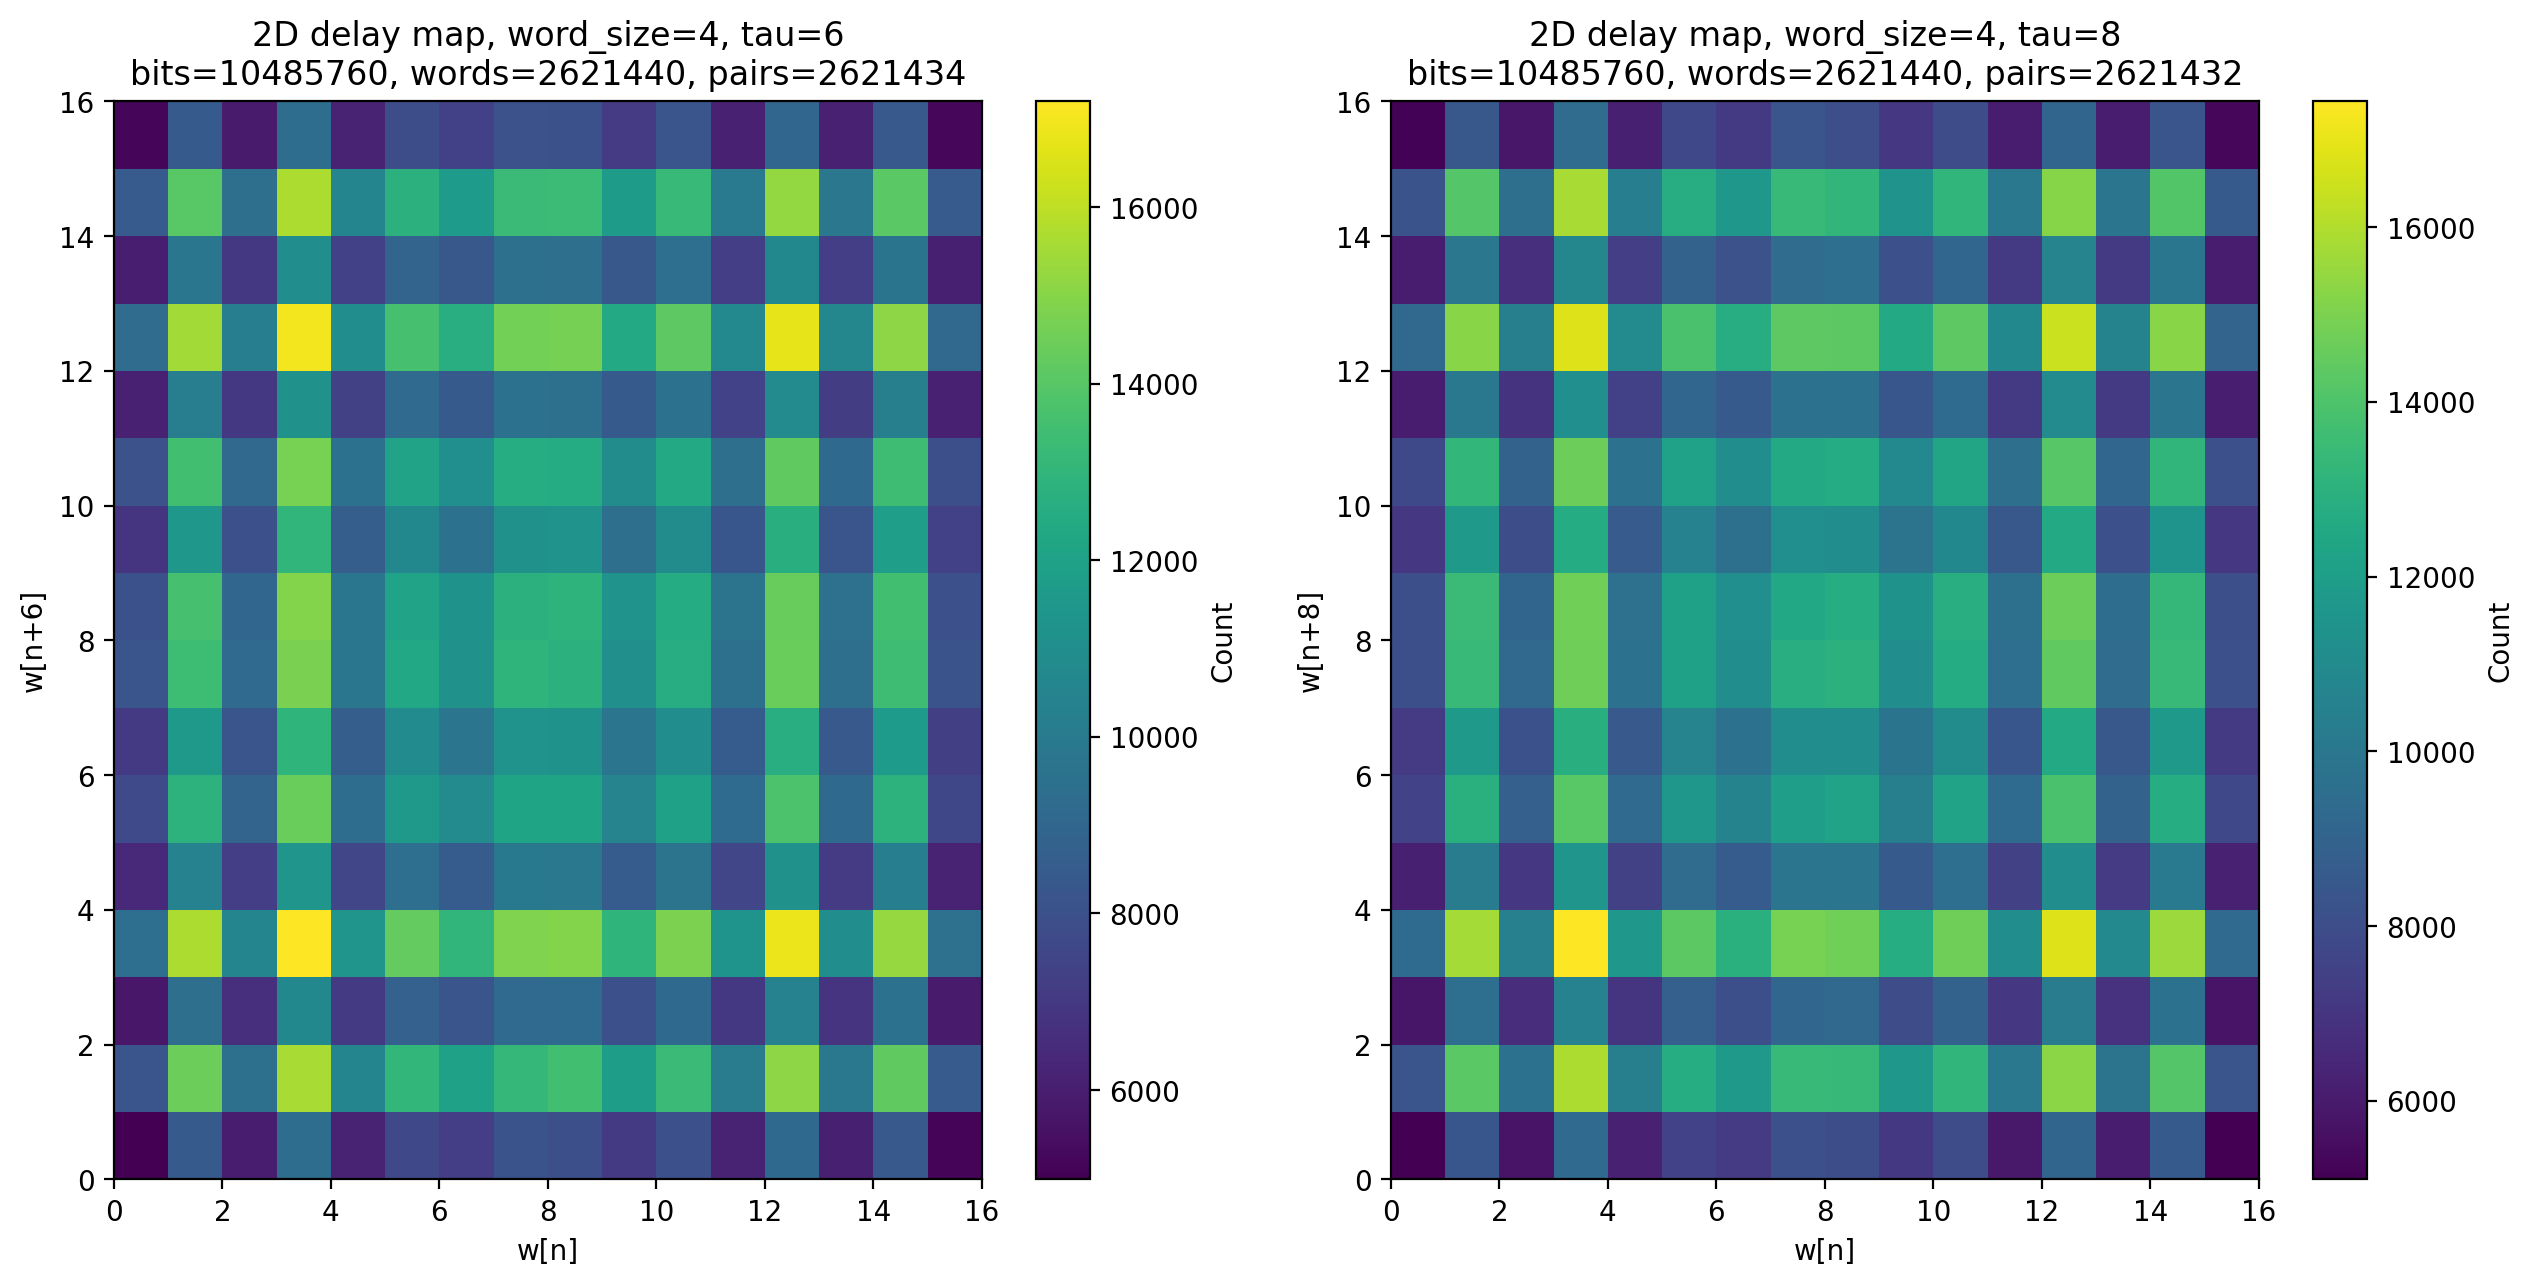
\includegraphics[width=0.70\textwidth]{gfx/spread_2d_w4_t6_t8}
    \caption{Mapy 2D dla oscylatorów rozproszonych w strukturze układu, przy parametrach
    $word\_size = 4$ oraz $\tau = 6$, $\tau = 8$.}
    \label{fig:map2d_spread_w4}
\end{figure}

Dla słów czterobitowych widoczny jest regularny układ jaśniejszych i ciemniejszych pasów
biegnących zarówno poziomo, jak i pionowo. Rozkład ten nie jest przypadkowy: podwyższone
zliczenia występują dla wartości słów o numerach 3, 12 oraz sąsiadujących z nimi,
natomiast wyraźnie obniżone dla wartości skrajnych, to jest 0 i 15. Odpowiada to
odpowiednio kombinacjom bitów o naprzemiennej strukturze oraz kombinacjom złożonym
z bitów jednakowych. Obraz ten stanowi bezpośrednie potwierdzenie wniosku sformułowanego
przy analizie autokorelacji, gdzie dla tej konfiguracji odnotowano silne ujemne
współczynniki w zakresie małych opóźnień: skłonność strumienia do naprzemiennej zmiany
wartości bitów przekłada się na uprzywilejowanie tych wartości słów, w których bity
sąsiednie się różnią, oraz na rzadsze występowanie słów o bitach jednakowych.
Zestawienie map dla dwóch różnych opóźnień pozwala rozdzielić dwa efekty. Struktura pasowa
jest praktycznie identyczna dla $\tau = 6$ i $\tau = 8$, co oznacza, że wynika ona z
rozkładu prawdopodobieństwa pojedynczych słów, a nie z zależności pomiędzy słowami
oddalonymi o zadane opóźnienie. Mapa dwuwymiarowa jest w tym przypadku w przybliżeniu
iloczynem dwóch identycznych rozkładów brzegowych, co odpowiada wzajemnej niezależności
obu współrzędnych przy jednoczesnym odstępstwie każdej z nich od rozkładu równomiernego.

\begin{figure}[ht]
    \centering
    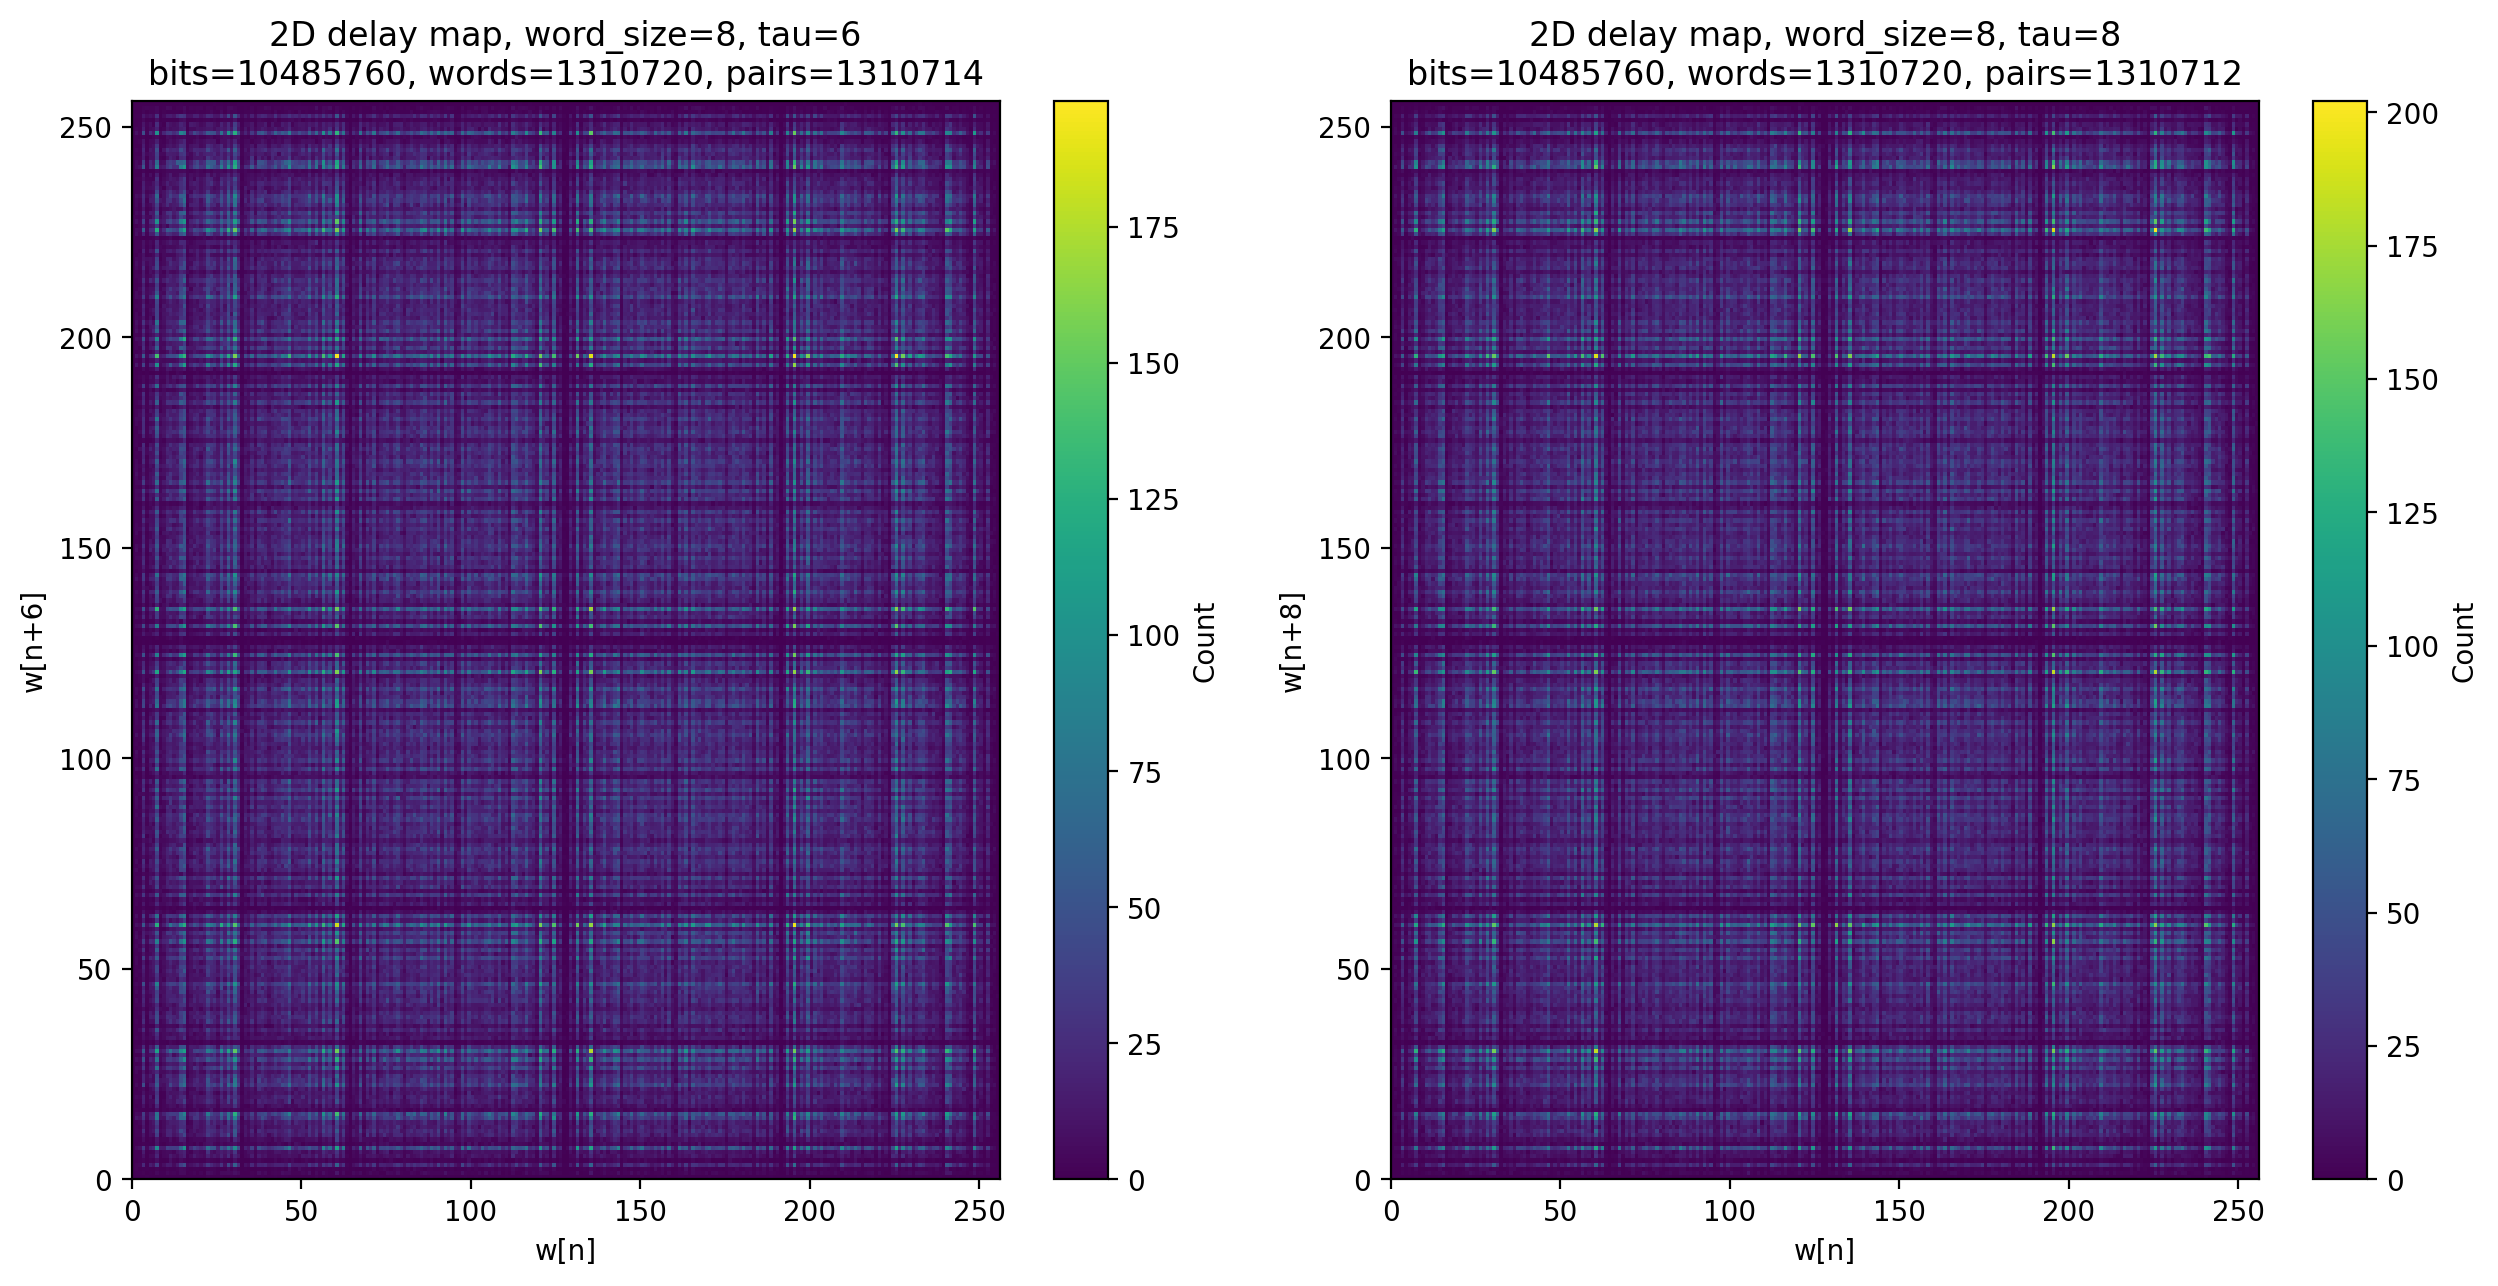
\includegraphics[width=0.98\textwidth]{gfx/spread_2d_w8_t6_t8}
    \caption{Mapy 2D dla oscylatorów rozproszonych w strukturze układu, przy parametrach
    $word\_size = 8$ oraz $\tau = 6$, $\tau = 8$.}
    \label{fig:map2d_spread_w8}
\end{figure}

Mapy dla słów ośmiobitowych, przedstawione na rysunku~\ref{fig:map2d_spread_w8},
ujawniają tę samą prawidłowość w bardziej rozbudowanej postaci. Widoczna jest regularna
siatka linii o obniżonych zliczeniach, dzieląca obszar mapy na bloki o rozmiarze
odpowiadającym w przybliżeniu 32 oraz 64 jednostkom, a więc potęgom liczby dwa. Położenie
tych linii wskazuje na uprzywilejowanie określonych bitów w obrębie bajtu, co jest
oczekiwane wobec faktu, że kolejne pozycje bajtu wypełniane są bitami pochodzącymi od
różnych oscylatorów, pracujących z różnymi częstotliwościami. Nie odnotowano natomiast
podwyższonych zliczeń wzdłuż przekątnej, co potwierdza, że powtarzalność całych bajtów
po zadanym opóźnieniu nie występuje.

Porównanie z konfiguracją poprzednią prowadzi do wniosku, że ręczne rozmieszczenie
oscylatorów nie usunęło nierównomierności rozkładu wartości słów, lecz uczyniło ją
wyraźniejszą. Jest to spójne z wynikiem badania autokorelacji dla tej konfiguracji
i wskazuje, że źródłem obserwowanego efektu nie są warunki pracy poszczególnych
pierścieni, a sposób łączenia bitów pochodzących z wielu kanałów w bajty wyjściowe.

\FloatBarrier

\subsection{Mapy dla 16 oscylatorów łączonych parami operacją XOR}

W konfiguracji obejmującej szesnaście oscylatorów, których wyjścia łączone są parami
operacją XOR, obraz map dwuwymiarowych zmienia się zasadniczo. Mapy dla słów
czterobitowych przedstawiono na rysunku~\ref{fig:map2d_xor_w4}.

\begin{figure}[ht]
    \centering
    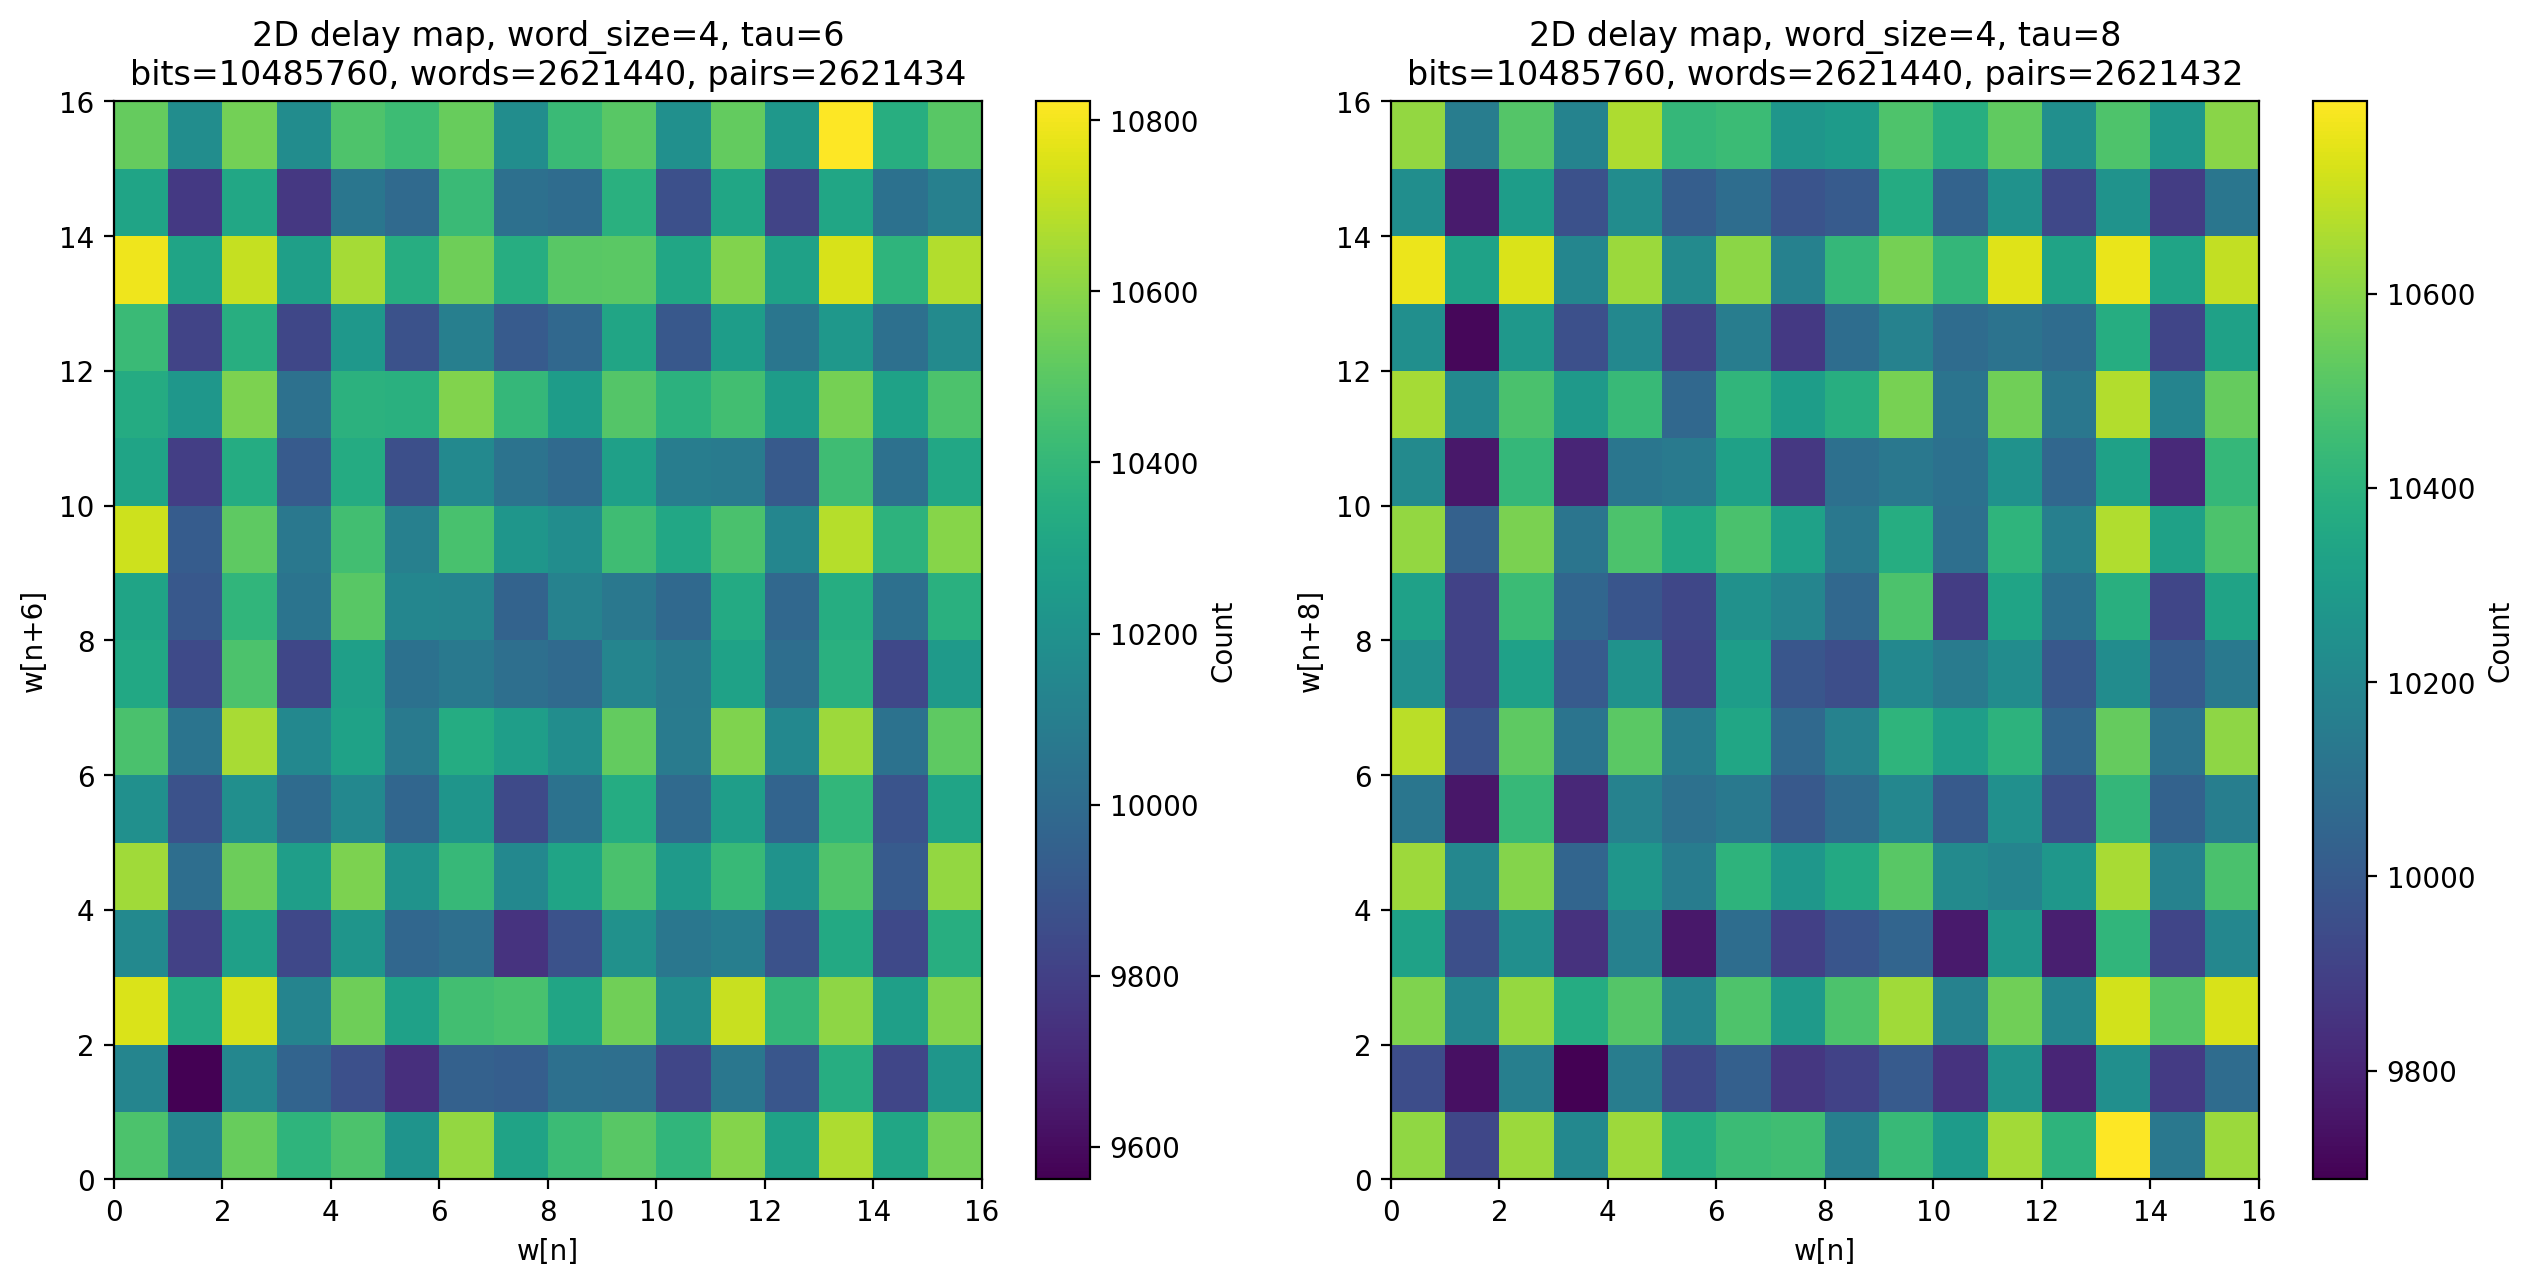
\includegraphics[width=0.98\textwidth]{gfx/xor_2d_w4_t6_t8}
    \caption{Mapy 2D dla 16 oscylatorów łączonych parami operacją XOR, przy parametrach
    $word\_size = 4$ oraz $\tau = 6$, $\tau = 8$.}
    \label{fig:map2d_xor_w4}
\end{figure}

Regularna struktura pasowa, dominująca w poprzednich konfiguracjach, przestała być
widoczna. Zliczenia rozkładają się nieregularnie w całym obszarze mapy, bez
uprzywilejowania określonych wartości słów. Zasadnicza zmiana dotyczy jednak nie samego
układu jasnych i ciemnych komórek, lecz zakresu skali barwnej. Dla konfiguracji bez
łączenia operacją XOR zliczenia obejmowały przedział od około $5\,500$ do $17\,000$,
natomiast obecnie mieszczą się w przedziale od $9\,600$ do $10\,800$. Przy $2\,621\,434$
analizowanych parach i $256$ komórkach histogramu wartość oczekiwana wynosi około
$10\,240$ zliczeń, wobec czego odnotowane odchylenia nie przekraczają sześciu procent
tej wielkości, gdy poprzednio sięgały ponad sześćdziesięciu procent. Interpretacja map
wymaga zatem każdorazowego odczytania zakresu skali, ponieważ jest on dobierany
automatycznie do zawartości danych i mapa o silnym kontraście wizualnym może
przedstawiać rozkład bliższy równomiernemu niż mapa pozornie jednorodna.

Dla źródła w pełni losowego zliczenia w komórkach podlegają rozkładowi Poissona,
którego odchylenie standardowe jest równe pierwiastkowi z wartości oczekiwanej i wynosi
w tym przypadku około $101$ zliczeń. Zaobserwowany rozrzut, obejmujący przedział około
$\pm 600$ zliczeń wokół wartości średniej, odpowiada zatem blisko sześciu odchyleniom
standardowym, co oznacza, że rozkład wartości słów nadal odbiega od równomiernego,
choć skala tego odstępstwa zmalała o rząd wielkości.

\begin{figure}[ht]
    \centering
    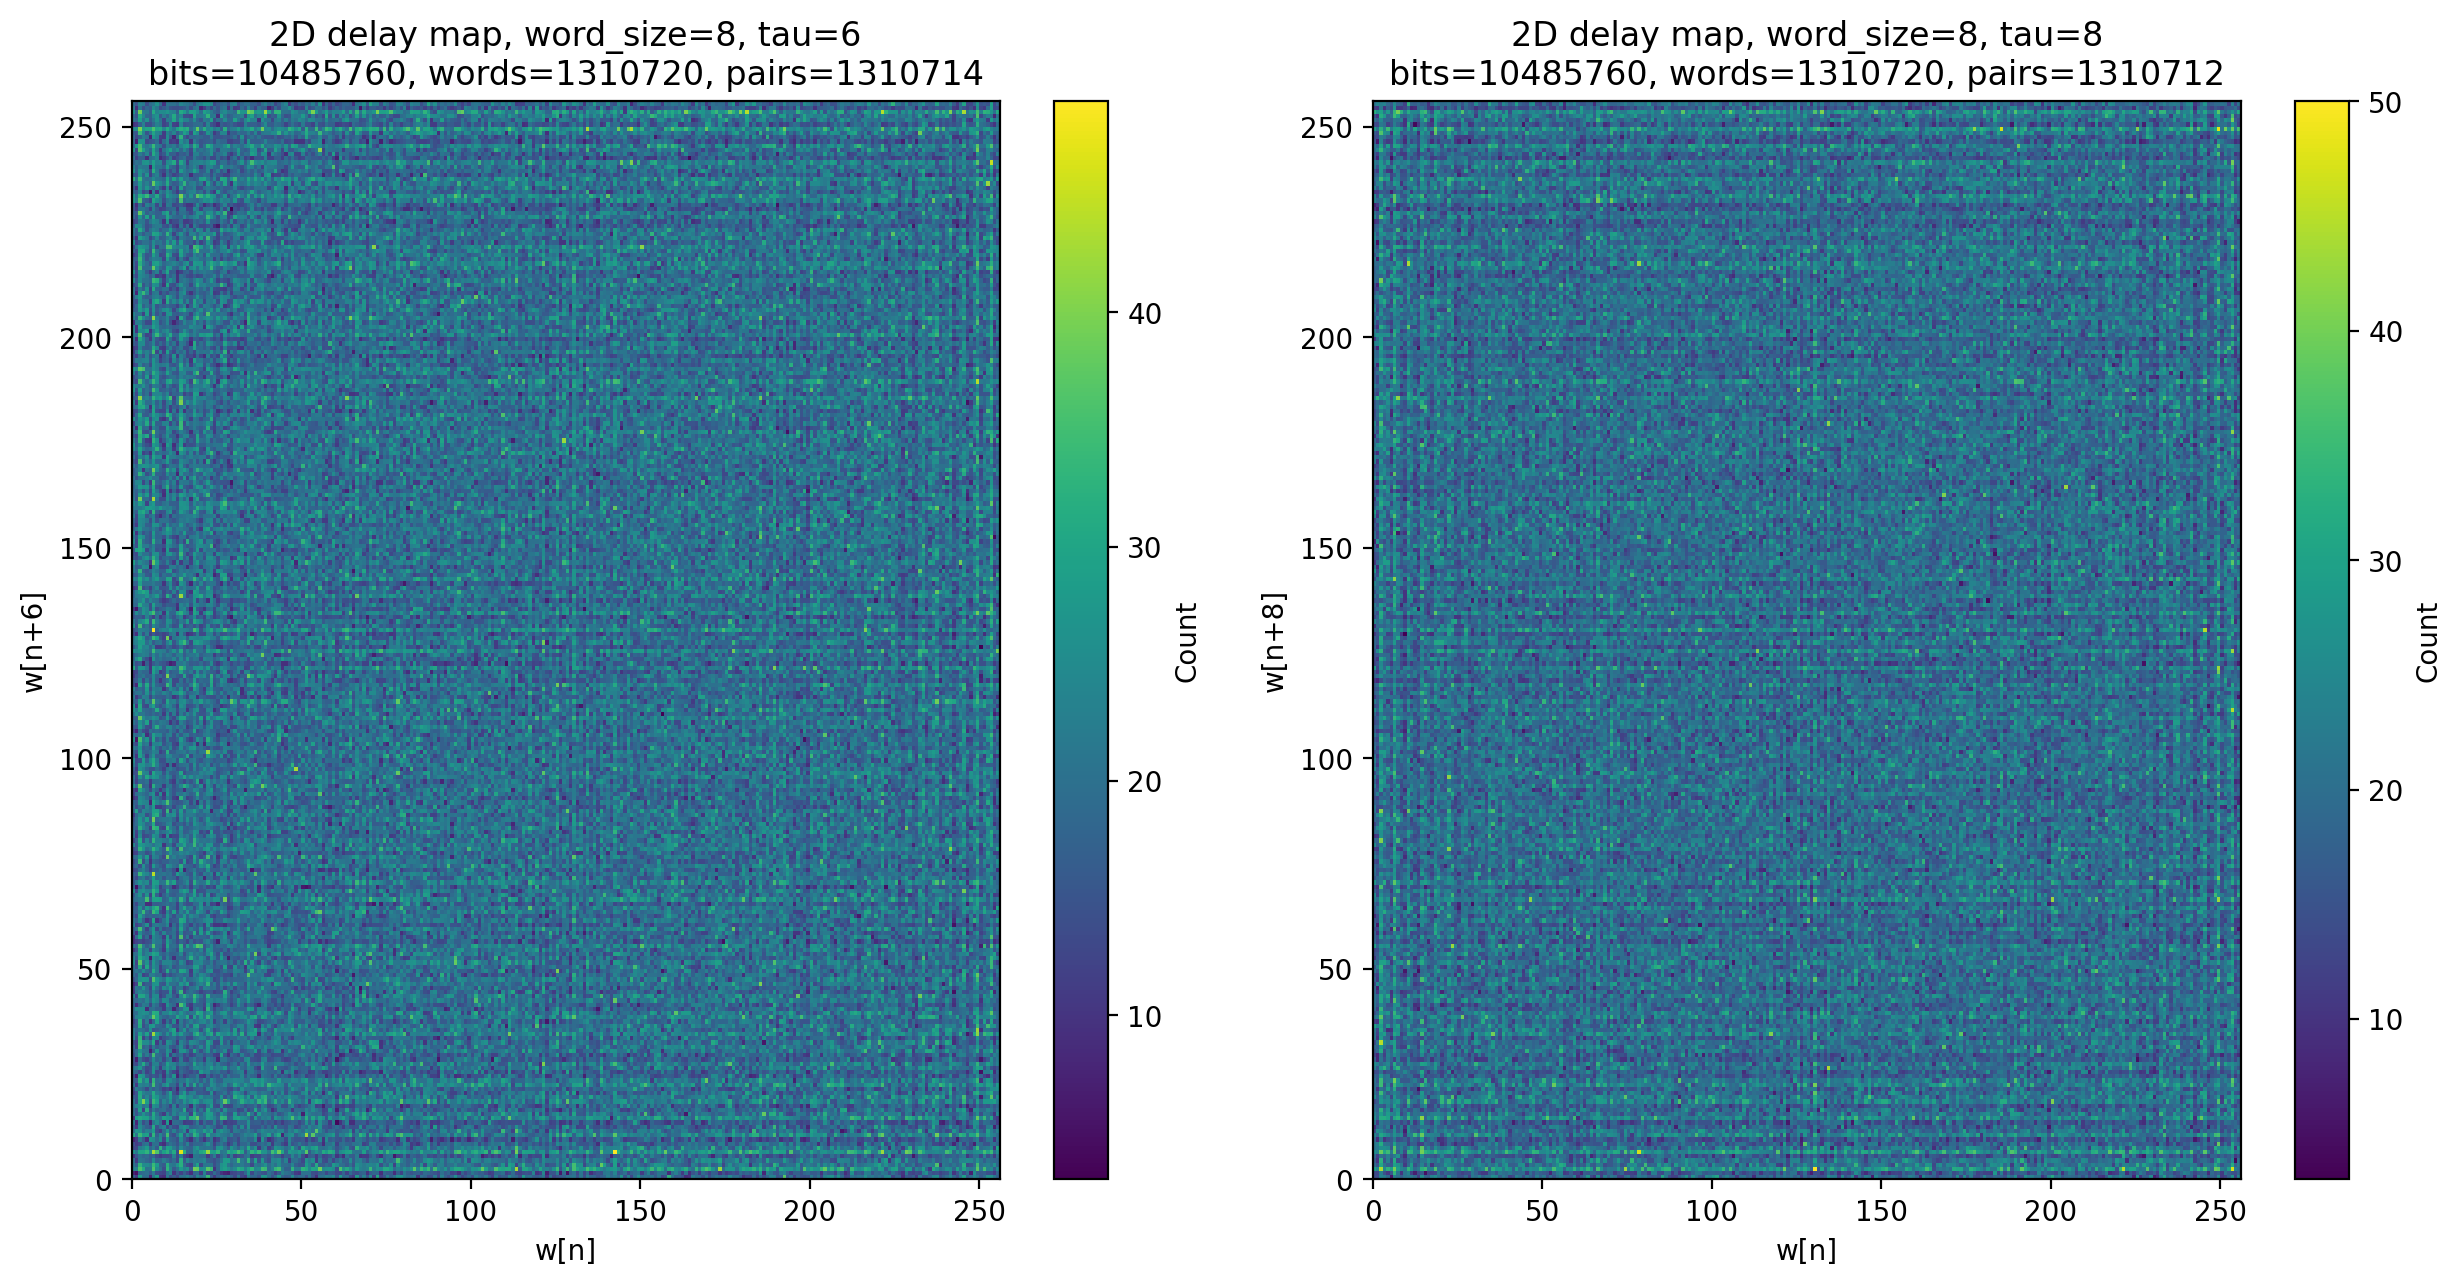
\includegraphics[width=0.98\textwidth]{gfx/xor_2d_w8_t6_t8}
    \caption{Mapy 2D dla 16 oscylatorów łączonych parami operacją XOR, przy parametrach
    $word\_size = 8$ oraz $\tau = 6$, $\tau = 8$.}
    \label{fig:map2d_xor_w8}
\end{figure}

Mapy dla słów ośmiobitowych, przedstawione na rysunku~\ref{fig:map2d_xor_w8}, mają
charakter drobnoziarnistego szumu, bez widocznej siatki linii o obniżonych zliczeniach,
obecnej w konfiguracjach poprzednich. Pewne pozostałości struktury dają się dostrzec
w postaci nieznacznie jaśniejszych pasm przy krawędziach obszaru, odpowiadających
wartościom bajtów o skrajnie małych i skrajnie dużych numerach. Przy $1\,310\,712$
parach rozłożonych na $65\,536$ komórek wartość oczekiwana zliczenia wynosi jedynie
około dwudziestu, a odpowiadające jej odchylenie standardowe około czterech i pół,
wobec czego znaczna część widocznego kontrastu jest naturalnym rozrzutem statystycznym,
nie zaś cechą generatora. Przy tak małej liczbie zliczeń na komórkę mapa dla słów
ośmiobitowych traci wartość diagnostyczną i pełni funkcję głównie jakościową,
potwierdzając brak wyraźnych struktur wielkoskalowych.

W żadnej z przedstawionych map nie występują podwyższone zliczenia wzdłuż przekątnej,
co oznacza brak skłonności do powtarzania tej samej wartości słowa po zadanym
opóźnieniu. Porównanie map dla $\tau = 6$ oraz $\tau = 8$ nie ujawnia istotnych różnic,
z czego wynika, że pozostałe odstępstwa od rozkładu równomiernego dotyczą
prawdopodobieństw wystąpienia poszczególnych wartości słów, a nie zależności pomiędzy
słowami oddalonymi w strumieniu.

\FloatBarrier

\subsection{Mapy dla 16 oscylatorów z wybielaniem metodą von Neumanna}

Ostatnią analizę wykonano dla tej samej serii pomiarowej co poprzednio, poddanej
wybielaniu metodą von Neumanna. Skrócenie strumienia do $2\,620\,032$ bitów zmniejsza
liczbę analizowanych par, a tym samym wartość oczekiwaną zliczenia w komórce histogramu,
co należy uwzględnić przy porównywaniu zakresów skali barwnej z mapami wcześniejszymi.
Mapy dla słów czterobitowych przedstawiono na rysunku~\ref{fig:map2d_vn_w4}.

\begin{figure}[ht]
    \centering
    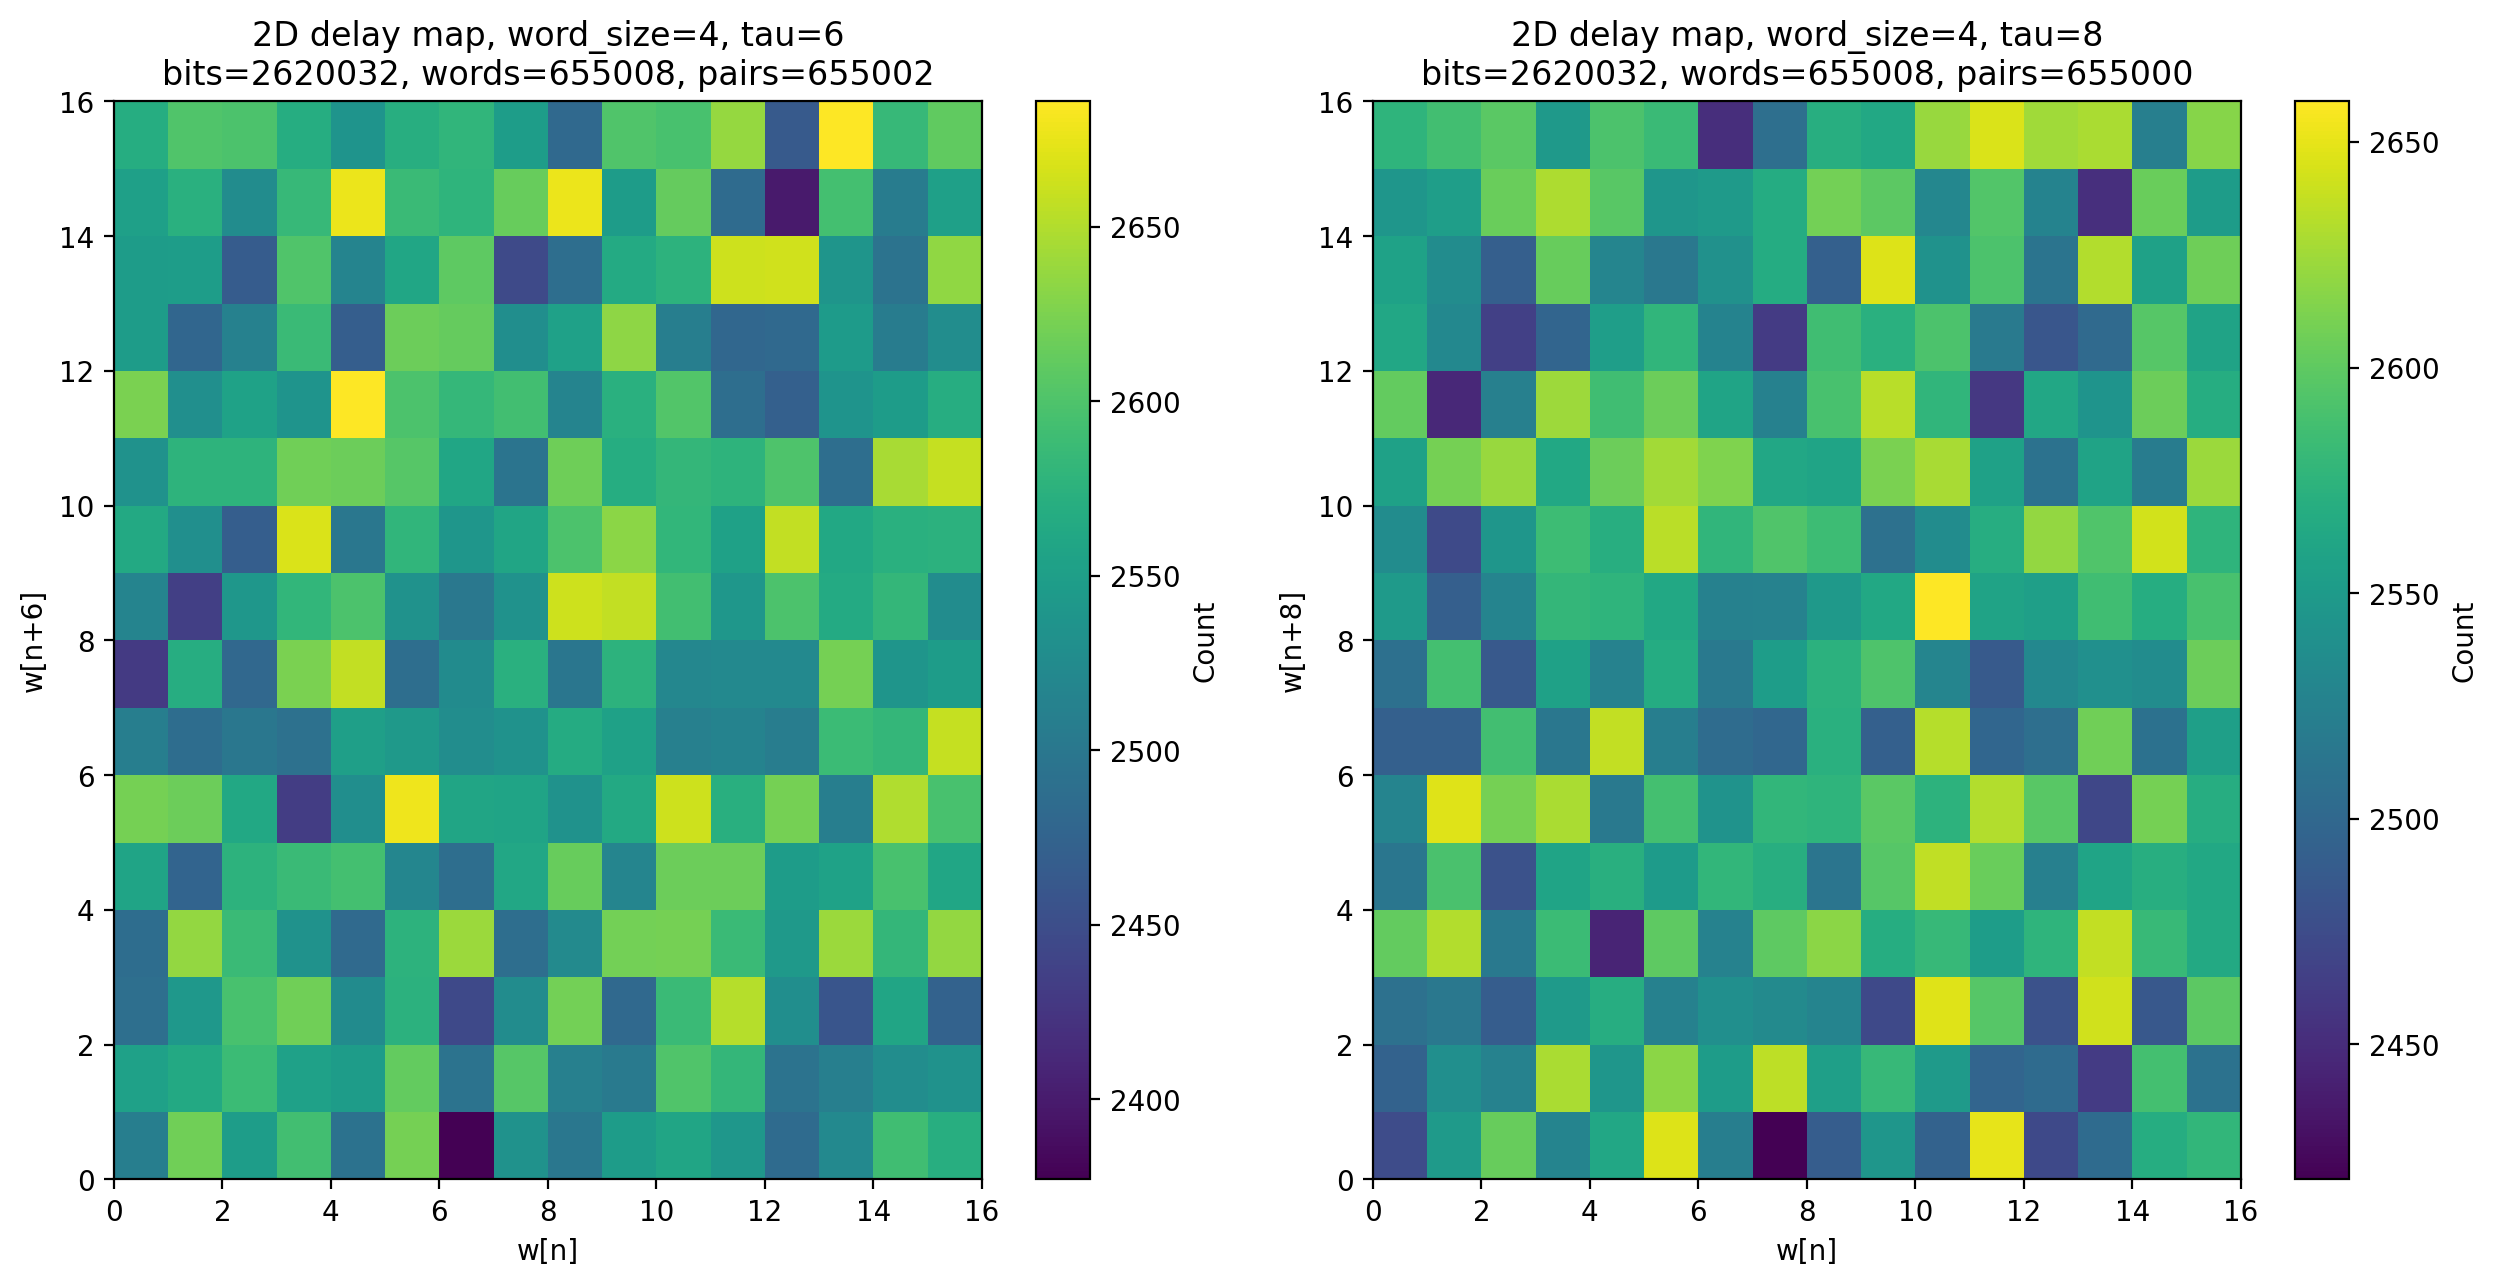
\includegraphics[width=0.98\textwidth]{gfx/vn_2d_w4_t6_t8}
    \caption{Mapy 2D dla 16 oscylatorów łączonych parami operacją XOR, po wybielaniu
    metodą von Neumanna, przy parametrach $word\_size = 4$ oraz $\tau = 6$, $\tau = 8$.}
    \label{fig:map2d_vn_w4}
\end{figure}

Dla słów czterobitowych liczba par wynosi $655\,002$, co przy $256$ komórkach histogramu
daje wartość oczekiwaną około $2\,559$ zliczeń oraz odpowiadające jej odchylenie
standardowe rozkładu Poissona równe około $51$ zliczeniom. Odnotowany zakres zliczeń,
obejmujący przedział od około $2\,390$ do $2\,680$, odpowiada zatem odchyleniu skrajnemu
na poziomie $3{,}3$ odchylenia standardowego dla $\tau = 6$ oraz $2{,}7$ dla $\tau = 8$.
Jest to wynik istotnie lepszy od uzyskanego dla strumienia surowego, w którym odchylenie
skrajne sięgało blisko sześciu odchyleń standardowych. Przy $256$ jednocześnie
analizowanych komórkach wartość maksymalna rzędu trzech odchyleń standardowych jest
zgodna z oczekiwaniem dla rozkładu równomiernego, wobec czego dla tej długości słowa nie
stwierdzono istotnego odstępstwa od losowości.

Porównanie z konfiguracją bez wybielania prowadzi do wniosku, że resztkowa
nierównomierność rozkładu wartości słów, obserwowana w strumieniu surowym, wynikała
w znacznej części z odchylenia prawdopodobieństwa pojedynczych bitów, a nie z zależności
strukturalnych. Metoda von Neumanna, usuwając odchylenie rozkładu, zredukowała je do
poziomu naturalnych fluktuacji statystycznych. Jest to spójne z wynikiem analizy
autokorelacji dla tej konfiguracji, gdzie po wybielaniu również nastąpił zanik
uporządkowanej struktury współczynników.

\begin{figure}[ht]
    \centering
    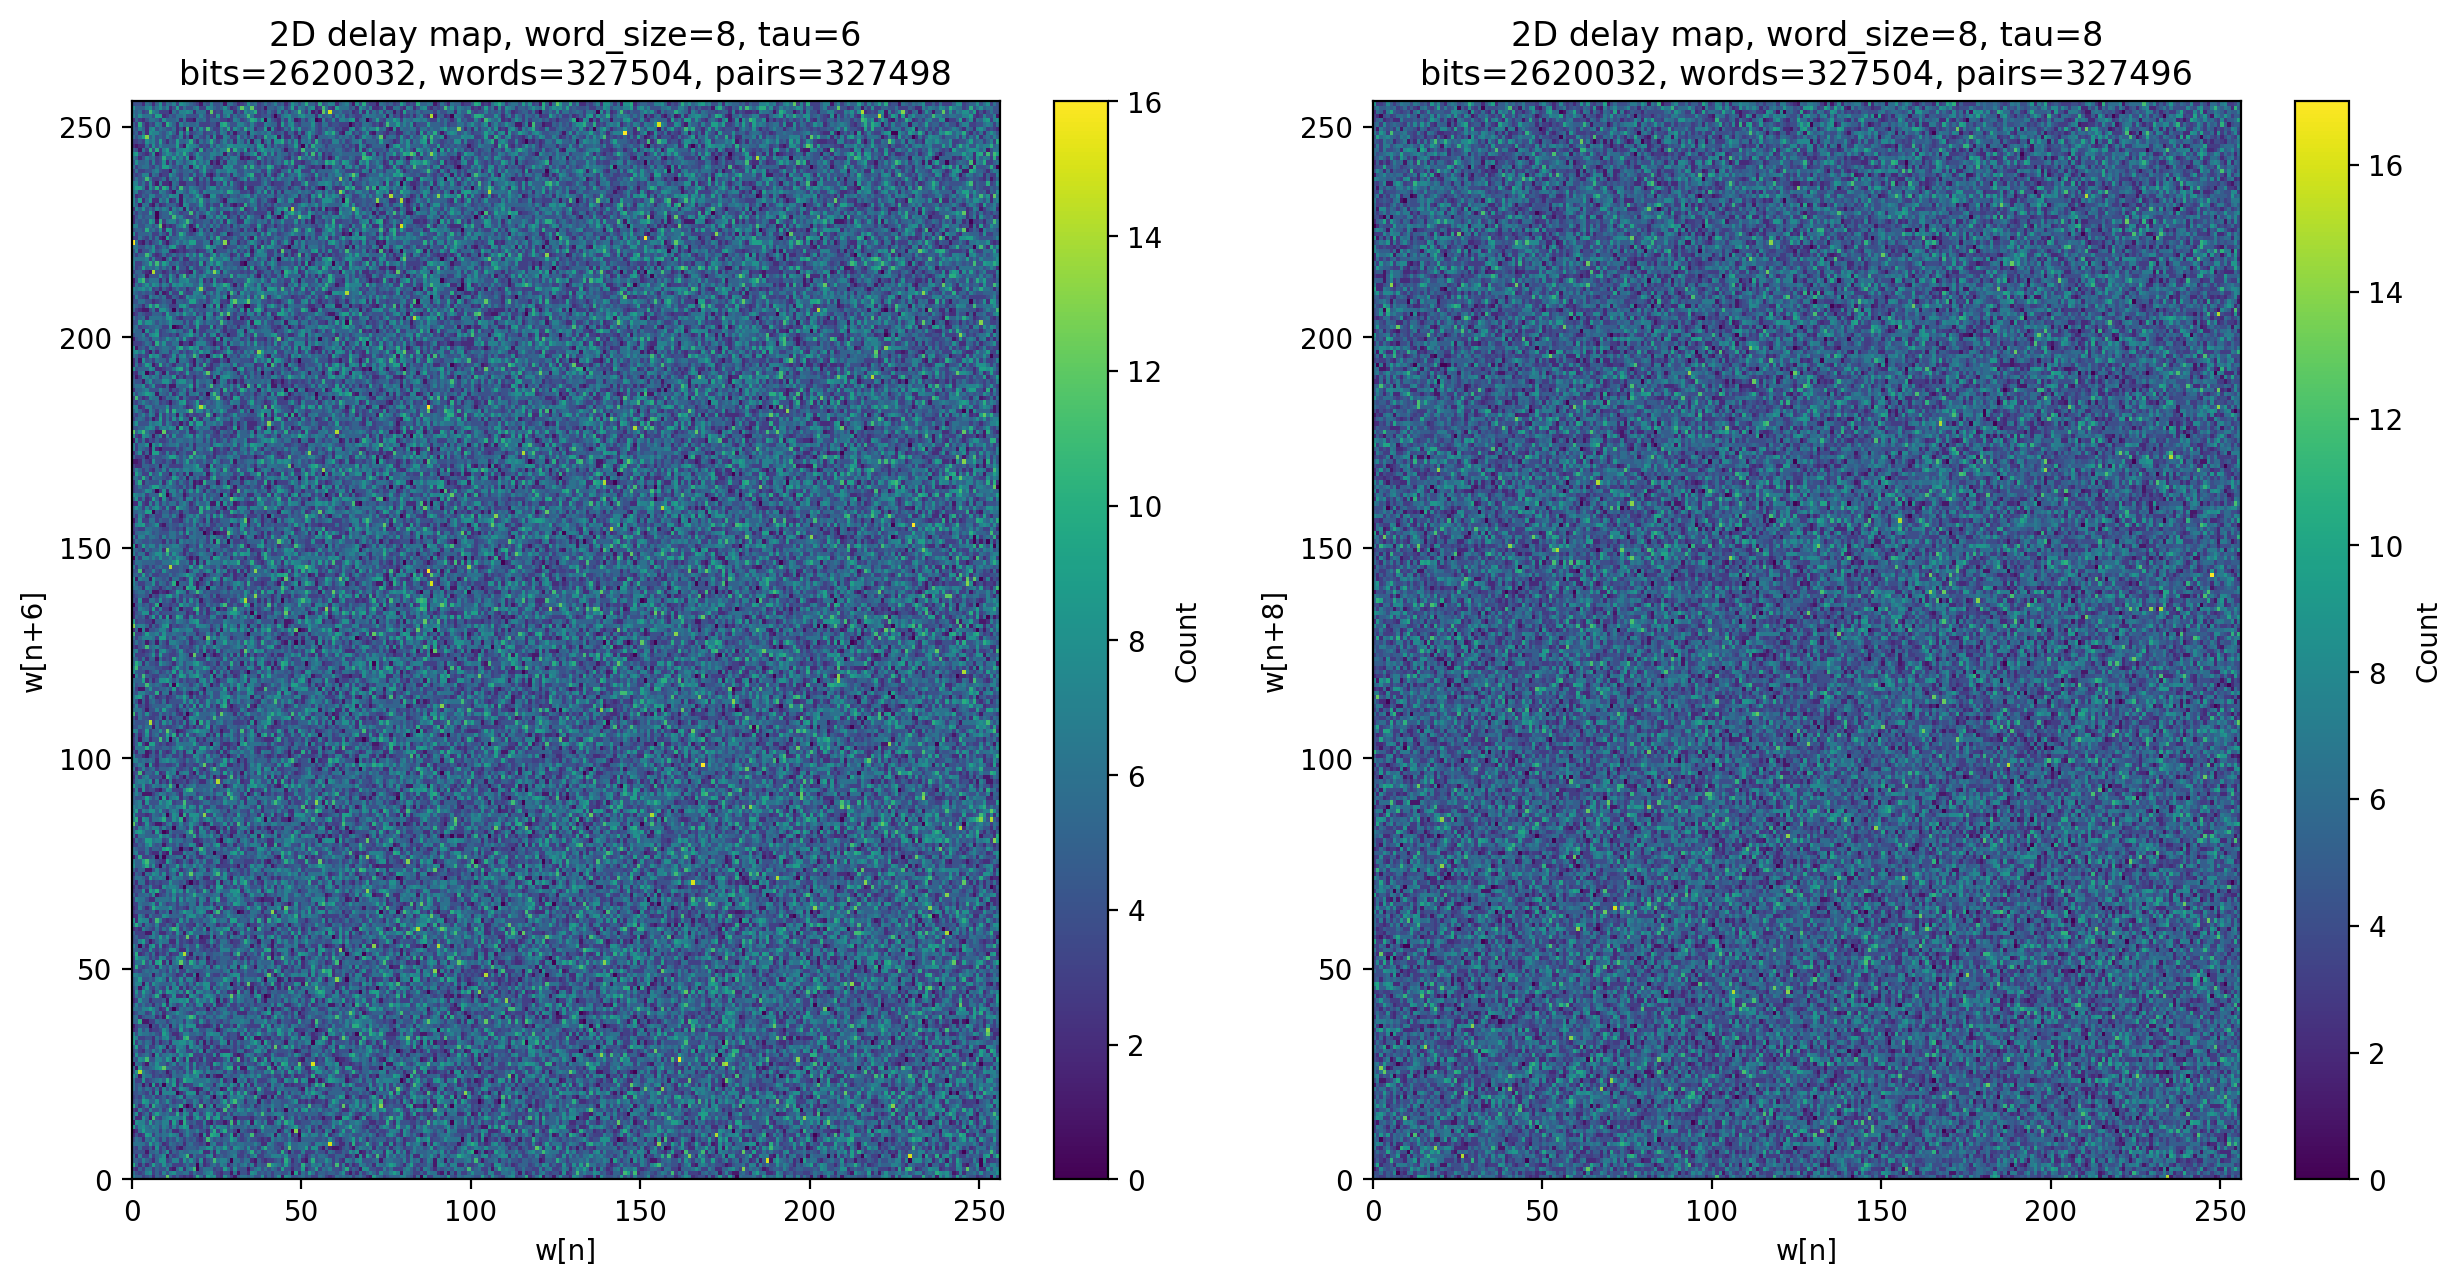
\includegraphics[width=0.98\textwidth]{gfx/vn_2d_w8_t6_t8}
    \caption{Mapy 2D dla 16 oscylatorów łączonych parami operacją XOR, po wybielaniu
    metodą von Neumanna, przy parametrach $word\_size = 8$ oraz $\tau = 6$, $\tau = 8$.}
    \label{fig:map2d_vn_w8}
\end{figure}

Mapy dla słów ośmiobitowych, przedstawione na rysunku~\ref{fig:map2d_vn_w8}, mają
charakter jednorodnego szumu bez żadnych struktur wielkoskalowych. Liczba par wynosi
w tym przypadku $327\,498$, co przy $65\,536$ komórkach daje wartość oczekiwaną zaledwie
pięciu zliczeń na komórkę. Przy tak małej liczności mapa przestaje pełnić funkcję
narzędzia pomiarowego: pojedyncze komórki puste oraz komórki o kilkunastu zliczeniach są
w tych warunkach zjawiskiem naturalnym, a nie oznaką wadliwości generatora. Widoczny
zakres skali, od zera do siedemnastu zliczeń, odpowiada odchyleniu skrajnemu rzędu pięciu
odchyleń standardowych, jednak przy $65\,536$ komórkach rozpatrywanych jednocześnie
wystąpienie takiej wartości jest oczekiwane. Mapa ta potwierdza zatem jedynie brak
struktur wielkoskalowych i nie pozwala na ilościową ocenę rozkładu.

Wynik ten wskazuje na istotne ograniczenie metody map dwuwymiarowych: użyteczna długość
słowa jest ograniczona przez długość serii pomiarowej. Aby uzyskać dla słów
ośmiobitowych liczność porównywalną z tą, jaką zapewniają słowa czterobitowe, seria
musiałaby być około dwustukrotnie dłuższa. Przy analizie strumieni poddanych wybielaniu,
skracającemu dane do jednej czwartej długości, ograniczenie to staje się szczególnie
wyraźne. Z tego względu w dalszej ocenie badanego generatora za miarodajne przyjęto
wyniki uzyskane dla słów czterobitowych, natomiast mapy dla słów ośmiobitowych
traktowano jako uzupełnienie o charakterze jakościowym.

\FloatBarrier

\section{Badanie odchylenia rozkładu bitów}

Kolejnym etapem praktycznej oceny generatora było zbadanie odchylenia rozkładu, czyli
nierównowagi pomiędzy liczbą zer i jedynek w uzyskanym strumieniu bitów. Badanie to
sprawdza, czy wyjście układu FPGA nie wykazuje przesunięcia w stronę jednej z wartości
logicznych. Jest to istotne szczególnie na etapie uruchamiania i strojenia generatora,
ponieważ asymetria może wskazywać na wpływ implementacji sprzętowej, sposobu próbkowania
lub parametrów zastosowanych oscylatorów pierścieniowych na jakość źródła entropii.

\subsection{Wyniki dla 8 oscylatorów rozmieszczonych automatycznie}

Badanie wykonano dla strumienia o długości $10\,485\,760$ bitów, pochodzącego
z~konfiguracji obejmującej osiem oscylatorów pierścieniowych rozmieszczonych
automatycznie przez narzędzie implementacyjne, bez łączenia wyjść operacją XOR
i~bez wybielania. Wyniki zestawiono w~tabeli~\ref{tab:bias_ro8}.

\begin{table}[ht]
    \centering
    \caption{Wyniki badania odchylenia rozkładu dla 8 oscylatorów rozmieszczonych
    automatycznie}
    \label{tab:bias_ro8}
    \small
    \begin{tabular}{lr}
        \toprule
        Parametr & Wartość \\
        \midrule
        Długość serii            & $10\,485\,760$ \\
        Liczba zer               & $5\,224\,958$ \\
        Liczba jedynek           & $5\,260\,802$ \\
        $P(0)$                   & $0{,}498291$ \\
        $P(1)$                   & $0{,}501709$ \\
        Bias $P(1)-0{,}5$        & $+0{,}001709$ \\
        Średnia w $\{-1,+1\}$    & $+0{,}003418$ \\
        $\sigma$                 & $1{,}54 \cdot 10^{-4}$ \\
        Odchylenie w jednostkach $\sigma$ & $11{,}1$ \\
        \bottomrule
    \end{tabular}
\end{table}

W badanym strumieniu występuje przewaga jedynek nad zerami, wynosząca $35\,844$ bity.
W~ujęciu bezwzględnym odchylenie jest niewielkie, ponieważ $P(1) = 0{,}501709$, a~więc
odstępstwo od wartości idealnej wynosi około $0{,}17\%$. Ocena istotności tego wyniku
wymaga jednak odniesienia do długości serii. Odchylenie standardowe udziału jedynek dla
źródła idealnie zrównoważonego wynosi $\sigma = 1/(2\sqrt{N}) \approx 1{,}54 \cdot
10^{-4}$, wobec czego stwierdzone odchylenie odpowiada $11{,}1$ odchylenia standardowego.

Wartość $p$ wykazana w~tabeli jako zero jest w~istocie wynikiem zaokrąglenia do sześciu
miejsc po przecinku; rzeczywista wartość jest rzędu $10^{-28}$. Oznacza to, że
prawdopodobieństwo zaobserwowania takiego odchylenia w~strumieniu pochodzącym ze źródła
idealnie zrównoważonego jest praktycznie zerowe, a~test monobitowy przy poziomie
istotności $\alpha = 0{,}01$ zostaje jednoznacznie odrzucony. Odchylenie ma zatem
charakter systematyczny i~jest cechą badanej implementacji, a~nie efektem przypadkowych
fluktuacji.

Kierunek odchylenia jest zgodny z~oczekiwaniami wynikającymi z~zasady działania
zastosowanego układu ekstrakcji entropii. Bity generowane są na podstawie detekcji zboczy,
przy czym zbocze narastające interpretowane jest jako zero, a~opadające jako jedynka.
Przewaga jedynek oznacza więc, że w~próbkowanym przebiegu częściej rejestrowane były
zbocza opadające, co odpowiada niesymetrycznemu współczynnikowi wypełnienia sygnału
z~oscylatorów. Zjawisko to wynika z~różnicy czasów propagacji zbocza narastającego
i~opadającego w~generatorach funkcji realizujących łańcuch inwerterów i~jest właściwością
technologiczną struktury układu, niezależną od sposobu opisu logiki w~języku HDL.

Uzyskany wynik wskazuje, że strumień w~postaci surowej nie spełnia wymagań stawianych
źródłom losowości i~wymaga zastosowania etapu korekcji rozkładu. Jednocześnie stwierdzone
odchylenie jest na tyle niewielkie w~ujęciu bezwzględnym, że korekcja metodą von Neumanna
powinna je usunąć przy niemal minimalnej stracie przepustowości, ponieważ udział par
odrzucanych rośnie z~kwadratem odchylenia i~dla wartości rzędu tysięcznych części pozostaje
praktycznie nierozróżnialny od przypadku granicznego. Skuteczność tego rozwiązania,
a~także wpływ liczby oscylatorów oraz łączenia ich wyjść operacją XOR na wielkość
odchylenia, przedstawiono w~kolejnych podrozdziałach.

\FloatBarrier

\subsection{Wyniki dla 8 oscylatorów rozmieszczonych ręcznie}

W kolejnej konfiguracji zachowano liczbę oscylatorów oraz długości ich łańcuchów
inwerterów, zmieniając wyłącznie sposób rozmieszczenia struktur, które narzucono ręcznie
w~oddalonych obszarach logiki programowalnej. Wyniki badania odchylenia rozkładu
zestawiono w~tabeli~\ref{tab:bias_ro8_manual}.

\begin{table}[ht]
    \centering
    \caption{Wyniki badania odchylenia rozkładu dla 8 oscylatorów rozmieszczonych ręcznie}
    \label{tab:bias_ro8_manual}
    \small
    \begin{tabular}{lr}
        \toprule
        Parametr & Wartość \\
        \midrule
        Długość serii            & $10\,485\,760$ \\
        Liczba zer               & $5\,241\,251$ \\
        Liczba jedynek           & $5\,244\,509$ \\
        $P(0)$                   & $0{,}499845$ \\
        $P(1)$                   & $0{,}500155$ \\
        Bias $P(1)-0{,}5$        & $+0{,}000155$ \\
        Średnia w $\{-1,+1\}$    & $+0{,}000311$ \\
        $\sigma$                 & $1{,}54 \cdot 10^{-4}$ \\
        Odchylenie w jednostkach $\sigma$ & $1{,}0$ \\
        Wartość $p$              & $0{,}314356$ \\
        \bottomrule
    \end{tabular}
\end{table}

Zmiana rozmieszczenia oscylatorów przyniosła bardzo wyraźną poprawę w~tej metryce.
Przewaga jedynek nad zerami zmalała z~$35\,844$ do $3\,258$ bitów, a~wartość biasu
z~$+0{,}001709$ do $+0{,}000155$, czyli ponad jedenastokrotnie. Stwierdzone odchylenie
odpowiada dokładnie jednemu odchyleniu standardowemu, a~więc mieści się w~zakresie
naturalnych fluktuacji statystycznych, jakich należy oczekiwać nawet od źródła idealnie
zrównoważonego. Potwierdza to wartość $p$ równa $0{,}314$, znacznie przewyższająca
przyjęty poziom istotności $\alpha = 0{,}01$: test monobitowy nie daje żadnych podstaw
do odrzucenia hipotezy o~zrównoważeniu strumienia.

Wynik ten jest tym bardziej wart uwagi, że kierunek odchylenia pozostał niezmieniony,
a~zmieniła się wyłącznie jego skala. Wskazuje to, że mechanizm odpowiedzialny za
asymetrię, czyli różnica czasów propagacji obu rodzajów zboczy, nie zniknął, lecz jego
wpływ na strumień wypadkowy uległ znacznemu osłabieniu. Prawdopodobnym wyjaśnieniem jest
zróżnicowanie warunków pracy poszczególnych pierścieni po ich rozproszeniu w~strukturze
układu. W~konfiguracji poprzedniej, w~której narzędzie implementacyjne umieściło wszystkie
oscylatory w~zwartym obszarze, struktury pracowały w~niemal identycznych warunkach,
wobec czego charakterystyczne dla nich odchylenia miały jednakowy kierunek i~sumowały się
w~strumieniu wyjściowym. Rozmieszczenie w~różnych obszarach struktury, obejmujących
odrębne regiony zegarowe i~różne fragmenty sieci dystrybucji zasilania, prowadzi do
zróżnicowania tych odchyleń, które w~sumie po ośmiu kanałach częściowo się kompensują.

Zestawienie tego wyniku z~wcześniejszą analizą autokorelacji prowadzi do obserwacji
istotnej dla całej pracy. Dla omawianej konfiguracji test monobitowy nie wykazuje
odstępstwa od losowości, natomiast badanie autokorelacji ujawniło w~tym samym strumieniu
zależności sięgające $270$ odchyleń standardowych, a~mapy dwuwymiarowe wyraźną
nierównomierność rozkładu wartości słów. Strumień o~praktycznie idealnie zrównoważonym
rozkładzie bitów może zatem jednocześnie zawierać silne i~łatwo wykrywalne zależności
pomiędzy kolejnymi pozycjami. Pokazuje to, że test monobitowy, choć jest naturalnym
pierwszym krokiem w~ocenie źródła losowości, bada wyłącznie rozkład brzegowy pojedynczych
bitów i~jego pozytywny wynik nie stanowi podstawy do stwierdzenia poprawności generatora.
Ocena jakości strumienia wymaga zastosowania metod badających strukturę czasową danych,
przy czym różne metody mogą prowadzić do odmiennego uszeregowania badanych konfiguracji.

\FloatBarrier

\subsection{Wyniki dla 16 oscylatorów łączonych parami operacją XOR}

W konfiguracji obejmującej szesnaście oscylatorów, których wyjścia łączone są parami
operacją XOR, badanie odchylenia rozkładu przeprowadzono na strumieniu surowym, bez
zastosowania wybielania. Wyniki zestawiono w~tabeli~\ref{tab:bias_ro16_xor}.

\begin{table}[ht]
    \centering
    \caption{Wyniki badania odchylenia rozkładu dla 16 oscylatorów łączonych parami
    operacją XOR}
    \label{tab:bias_ro16_xor}
    \small
    \begin{tabular}{lr}
        \toprule
        Parametr & Wartość \\
        \midrule
        Długość serii            & $10\,485\,760$ \\
        Liczba zer               & $5\,241\,014$ \\
        Liczba jedynek           & $5\,244\,746$ \\
        $P(0)$                   & $0{,}499822$ \\
        $P(1)$                   & $0{,}500178$ \\
        Bias $P(1)-0{,}5$        & $+0{,}000178$ \\
        Średnia w $\{-1,+1\}$    & $+0{,}000356$ \\
        $\sigma$                 & $1{,}54 \cdot 10^{-4}$ \\
        Odchylenie w jednostkach $\sigma$ & $1{,}2$ \\
        Wartość $p$              & $0{,}249115$ \\
        \bottomrule
    \end{tabular}
\end{table}

Odnotowana przewaga jedynek nad zerami wynosi $3\,732$ bity, a~wartość biasu
$+0{,}000178$, co odpowiada $1{,}2$ odchylenia standardowego. Wartość $p$ równa $0{,}249$
znacznie przewyższa przyjęty poziom istotności, wobec czego test monobitowy nie daje
podstaw do odrzucenia hipotezy o~zrównoważeniu strumienia.

Wynik ten jest praktycznie identyczny z~uzyskanym dla konfiguracji z~ośmioma oscylatorami
rozmieszczonymi ręcznie, gdzie bias wyniósł $+0{,}000155$, czyli $1{,}0$ odchylenia
standardowego. Różnica między obiema wartościami mieści się w~granicach naturalnego
rozrzutu i~nie pozwala stwierdzić, która konfiguracja jest w~tej metryce lepsza.
Obserwacja ta wymaga komentarza, ponieważ na pierwszy rzut oka pozostaje w~sprzeczności
z~oczekiwaniem teoretycznym. Połączenie dwóch niezależnych źródeł operacją XOR powinno
prowadzić do zmniejszenia odchylenia w~sposób multiplikatywny: przy odchyleniach
$\varepsilon_1$ oraz $\varepsilon_2$ odchylenie sygnału wynikowego wynosi
$2\varepsilon_1\varepsilon_2$, wobec czego dla wartości rzędu tysięcznych części
oczekiwane odchylenie po operacji XOR powinno być mniejsze o~kilka rzędów wielkości.

Wyjaśnieniem tej rozbieżności jest fakt, że dla obu konfiguracji stwierdzone odchylenie
znajduje się już na poziomie naturalnego rozrzutu statystycznego wyznaczonego długością
serii. Odchylenie standardowe $\sigma \approx 1{,}54 \cdot 10^{-4}$ stanowi w~tym
przypadku granicę czułości pomiaru: nawet gdyby operacja XOR zredukowała odchylenie
rzeczywiste do wartości pomijalnie małej, zmierzony bias pozostałby na poziomie rzędu
jednego $\sigma$, ponieważ wynikałby wówczas wyłącznie z~losowego rozrzutu liczby jedynek
w~skończonej próbie. Test monobitowy nie jest zatem zdolny rozróżnić tych dwóch
konfiguracji przy zastosowanej długości serii, a~stwierdzenie rzeczywistej poprawy
wymagałoby zebrania danych o~kilka rzędów wielkości dłuższych.

Niezależne potwierdzenie bardzo małego odchylenia dla omawianej konfiguracji przynosi
natomiast wydajność wybielania metodą von Neumanna, omówiona w~podrozdziale dotyczącym
autokorelacji. Udział bitów zachowanych po korekcji wyniósł $24{,}99\%$, a~więc
praktycznie tyle, ile wynosi granica teoretyczna dla źródła nieobciążonego. Ponieważ
udział par odrzucanych rośnie z~kwadratem odchylenia, wskaźnik ten jest czuły na bias
i~jego wartość potwierdza, że rzeczywiste odchylenie strumienia było w~tej konfiguracji
istotnie mniejsze, niż wskazuje sam wynik testu monobitowego.

Podsumowując, trzy z~czterech badanych konfiguracji różnią się w~zakresie odchylenia
rozkładu w~sposób jednoznaczny jedynie w~jednym przypadku: automatyczne rozmieszczenie
oscylatorów prowadziło do odchylenia na poziomie $11$ odchyleń standardowych, natomiast
wszystkie konfiguracje z~rozmieszczeniem ręcznym dają wyniki nierozróżnialne od źródła
zrównoważonego. Decydującym czynnikiem w~tej metryce okazało się zatem rozproszenie
struktur w~obrębie układu, a~nie liczba oscylatorów ani zastosowanie operacji XOR.

\FloatBarrier

\subsection{Wyniki dla 16 oscylatorów z wybielaniem metodą von Neumanna}

Ostatni pomiar wykonano dla tej samej serii pomiarowej co poprzednio, poddanej wybielaniu
metodą von Neumanna. Wyniki zestawiono w~tabeli~\ref{tab:bias_ro16_vn}.

\begin{table}[ht]
    \centering
    \caption{Wyniki badania odchylenia rozkładu dla 16 oscylatorów łączonych parami
    operacją XOR, po wybielaniu metodą von Neumanna}
    \label{tab:bias_ro16_vn}
    \small
    \begin{tabular}{lr}
        \toprule
        Parametr & Wartość \\
        \midrule
        Długość serii            & $2\,620\,032$ \\
        Liczba zer               & $1\,308\,483$ \\
        Liczba jedynek           & $1\,311\,549$ \\
        $P(0)$                   & $0{,}499415$ \\
        $P(1)$                   & $0{,}500585$ \\
        Bias $P(1)-0{,}5$        & $+0{,}000585$ \\
        Średnia w $\{-1,+1\}$    & $+0{,}001170$ \\
        $\sigma$                 & $3{,}09 \cdot 10^{-4}$ \\
        Odchylenie w jednostkach $\sigma$ & $1{,}9$ \\
        Wartość $p$              & $0{,}058203$ \\
        \bottomrule
    \end{tabular}
\end{table}

Test monobitowy przy poziomie istotności $\alpha = 0{,}01$ nie daje podstaw do odrzucenia
hipotezy o~zrównoważeniu strumienia, ponieważ wartość $p$ wynosi $0{,}058$. Wynik ten
wymaga jednak uważniejszej interpretacji, gdyż w~ujęciu bezwzględnym wartość biasu
wzrosła: z~$+0{,}000178$ dla strumienia surowego do $+0{,}000585$ po wybielaniu, a~więc
ponad trzykrotnie. Jest to obserwacja sprzeczna z~przeznaczeniem zastosowanej metody,
która ma odchylenie rozkładu usuwać, a~nie zwiększać.

Zasadnicza część tej rozbieżności ma charakter pozorny i~wynika ze skrócenia serii.
Wybielanie zredukowało długość strumienia do jednej czwartej, wobec czego odchylenie
standardowe wzrosło dwukrotnie, do $\sigma \approx 3{,}09 \cdot 10^{-4}$. Wyrażone
w~jednostkach naturalnego rozrzutu odchylenie wynosi zatem $1{,}9$ zamiast $1{,}2$,
a~więc wzrost jest znacznie mniej wyraźny niż w~ujęciu bezwzględnym i~mieści się
w~zakresie, jakiego można oczekiwać przy losowym rozrzucie. Porównywanie wartości biasu
pomiędzy seriami o~różnej długości bez takiego przeliczenia prowadziłoby do błędnych
wniosków, ponieważ każde skrócenie danych z~definicji zwiększa oczekiwaną wartość
bezwzględną zmierzonego odchylenia.

Pozostaje jednak pytanie, dlaczego wybielanie nie doprowadziło do wartości bliższej zeru,
skoro metoda von Neumanna gwarantuje idealne zrównoważenie strumienia wyjściowego.
Gwarancja ta obowiązuje wyłącznie przy założeniu wzajemnej niezależności kolejnych bitów
strumienia wejściowego. Tymczasem analiza autokorelacji wykazała dla tej konfiguracji
istnienie zależności w~zakresie małych opóźnień, przekraczających pięć odchyleń
standardowych. Przy skorelowanym strumieniu wejściowym pary o~różnych wartościach
przestają występować z~jednakowym prawdopodobieństwem, w~konsekwencji czego korekcja nie
usuwa odchylenia w~pełni. Stwierdzone po wybielaniu odchylenie na poziomie dwóch
odchyleń standardowych należy zatem traktować jako pośredni ślad zależności czasowych
obecnych w~strumieniu surowym, a~nie jako niedoskonałość samej implementacji korekcji.

Warto przy tym zauważyć, że mimo braku pełnego usunięcia odchylenia wybielanie
poprawiło wynik pozostałych zastosowanych metod: mapy dwuwymiarowe wykazały spadek
rozrzutu zliczeń z~około sześciu do niespełna trzech odchyleń standardowych, a~przebieg
autokorelacji utracił uporządkowaną strukturę. Metoda von Neumanna okazała się więc
skuteczna wobec tych odstępstw od losowości, których nie wykrywa test monobitowy,
pozostając jednocześnie bez wyraźnego wpływu na samą wielkość odchylenia rozkładu, która
w~konfiguracjach z~ręcznym rozmieszczeniem oscylatorów była już przed korekcją
nierozróżnialna od naturalnego rozrzutu.

\FloatBarrier

\section{Wnioski z analizy statystycznej generatora liczb losowych}

Przeprowadzona analiza objęła trzy metody: badanie autokorelacji strumienia bitów, mapy
dwuwymiarowe rozkładu słów oraz test odchylenia rozkładu bitów. Każdą z nich zastosowano
do czterech konfiguracji generatora, różniących się liczbą oscylatorów pierścieniowych,
sposobem ich rozmieszczenia w~strukturze układu, obecnością operacji XOR na wyjściach oraz
zastosowaniem korekcji metodą von Neumanna. Zestawienie uzyskanych wyników przedstawiono
w~tabeli~\ref{tab:synteza}, przy czym wszystkie wartości wyrażono w~jednostkach odchylenia
standardowego właściwego dla danej metody i~długości serii, co umożliwia porównywanie
pomiarów o~różnej liczności.

\begin{table}[htbp]
    \centering
    \caption{Zestawienie wyników wszystkich zastosowanych metod analizy. Wartości
    wyrażono w~jednostkach odchylenia standardowego}
    \label{tab:synteza}
    \small
    \begin{tabular}{clccc}
        \toprule
        Nr & Konfiguracja & Odchylenie rozkładu & Autokorelacja & Mapy 2D \\
        \midrule
        1 & 8 RO, rozmieszczenie automatyczne & $11{,}1$ & $3{,}8$   & $8{,}5$ \\
        2 & 8 RO, rozmieszczenie ręczne       & $1{,}0$  & $270$     & $67$ \\
        3 & 16 RO, XOR                        & $1{,}2$  & $9{,}8$   & $6$ \\
        4 & 16 RO, XOR, von Neumann           & $1{,}9$  & $3{,}2$   & $2{,}7$ \\
        \bottomrule
    \end{tabular}
\end{table}

Najistotniejszym wnioskiem wynikającym z~tego zestawienia jest brak zgodności pomiędzy
zastosowanymi metodami co do uszeregowania badanych konfiguracji. Konfiguracja pierwsza,
w~której oscylatory rozmieszczono automatycznie, wypadła najlepiej w~badaniu
autokorelacji, a~jednocześnie zdecydowanie najgorzej w~teście odchylenia rozkładu, gdzie
odnotowane odstępstwo sięgnęło jedenastu odchyleń standardowych i~doprowadziło do
odrzucenia hipotezy o~zrównoważeniu strumienia. Konfiguracja druga wykazała zależność
odwrotną: rozproszenie struktur zredukowało odchylenie rozkładu do poziomu naturalnych
fluktuacji, jednocześnie pogarszając wynik autokorelacji o~blisko dwa rzędy wielkości.
Żadna z~pojedynczych metod nie pozwoliłaby zatem na poprawną ocenę badanego źródła,
a~oparcie wniosków wyłącznie na teście monobitowym doprowadziłoby do zaakceptowania
strumienia zawierającego zależności czasowe wykrywalne na poziomie dwustu siedemdziesięciu
odchyleń standardowych.

Rozproszenie oscylatorów w~strukturze układu okazało się czynnikiem decydującym dla
odchylenia rozkładu. Wszystkie trzy konfiguracje z~rozmieszczeniem ręcznym dały wyniki
nierozróżnialne od źródła zrównoważonego, mieszczące się w~przedziale od jednego do dwóch
odchyleń standardowych, wobec jedenastu odchyleń dla rozmieszczenia automatycznego.
Wyjaśnieniem jest zróżnicowanie warunków pracy poszczególnych pierścieni: struktury
umieszczone w~zwartym obszarze pracują w~niemal identycznych warunkach temperaturowych
i~zasilania, wobec czego charakterystyczne dla nich asymetrie czasów propagacji zboczy
mają jednakowy kierunek i~sumują się w~strumieniu wypadkowym, natomiast po rozproszeniu
częściowo się kompensują. Ten sam zabieg pogorszył jednak wynik autokorelacji, ponieważ
zróżnicowanie lokalnych warunków pracy przekłada się na większy rozrzut częstotliwości
oscylatorów, a~przy stałej kolejności zapisu kanałów do bufora prowadzi to do powstania
wyraźniejszej struktury okresowej w~strumieniu wyjściowym.

Zwiększenie liczby oscylatorów do szesnastu wraz z~łączeniem ich wyjść operacją XOR
przyniosło znaczącą poprawę wyników obu metod badających strukturę danych: amplituda
zależności autokorelacyjnych zmalała blisko dwudziestoośmiokrotnie, a~rozrzut zliczeń na
mapach dwuwymiarowych z~sześćdziesięciu siedmiu do sześciu odchyleń standardowych. W~teście
odchylenia rozkładu nie stwierdzono natomiast różnicy względem konfiguracji poprzedniej,
co nie oznacza braku poprawy, lecz wynika z~ograniczonej czułości pomiaru: przy serii
o~długości $10\,485\,760$ bitów odchylenie standardowe wynosi $1{,}54 \cdot 10^{-4}$
i~stanowi granicę rozdzielczości, poniżej której test monobitowy nie różnicuje źródeł.
Pośrednim potwierdzeniem bardzo małego odchylenia dla tej konfiguracji jest wydajność
korekcji von Neumanna, wynosząca $24{,}99\%$ długości wejściowej, a~więc praktycznie równa
granicy teoretycznej osiąganej dla źródła nieobciążonego.

Zastosowanie korekcji metodą von Neumanna okazało się skuteczne wobec tych odstępstw od
losowości, których test monobitowy nie wykrywa. Po wybielaniu przebieg autokorelacji
utracił uporządkowaną strukturę obejmującą opóźnienia od dwóch do sześciu, a~rozrzut
zliczeń na mapach dwuwymiarowych spadł do poziomu poniżej trzech odchyleń standardowych,
zgodnego z~oczekiwaniem dla rozkładu równomiernego. Metoda nie zmniejszyła natomiast
samego odchylenia rozkładu, które pozostało na poziomie dwóch odchyleń standardowych.
Wynika to z~faktu, że korekcja von Neumanna gwarantuje zrównoważenie strumienia
wyjściowego wyłącznie przy założeniu wzajemnej niezależności bitów wejściowych, a~założenie
to nie było w~badanym strumieniu spełnione. Stwierdzone po wybielaniu odchylenie należy
zatem traktować jako pośredni ślad zależności czasowych obecnych w~danych surowych.

Analiza wskazała jednocześnie źródło zasadniczej części wykrytych odstępstw. We wszystkich
konfiguracjach zależności koncentrowały się w~zakresie opóźnień odpowiadających liczbie
kanałów doprowadzonych do modułu ekstrakcji entropii oraz długości bajtu, a~ich charakter
zmieniał się wraz z~relacjami częstotliwości pomiędzy oscylatorami, nie zaś wraz z~jakością
samych źródeł szumu. Wskazuje to na warstwę serializacji jako mechanizm odpowiedzialny za
powstawanie struktury okresowej: bity zapisywane są do bufora w~stałej kolejności numerów
kanałów, wobec czego uporządkowanie oscylatorów według częstotliwości pracy przekłada się
bezpośrednio na uporządkowanie wartości w~strumieniu wyjściowym.

Przy formułowaniu powyższych wniosków należy uwzględnić dwa ograniczenia przyjętej
metodyki. Przejście od konfiguracji drugiej do trzeciej obejmowało jednoczesną zmianę dwóch
parametrów, liczby oscylatorów oraz obecności operacji XOR, w~związku z~czym nie jest
możliwe rozdzielenie wpływu każdego z~nich na obserwowaną poprawę.

Jako kierunki dalszych prac zasadne wydają się trzy zagadnienia. Pierwszym jest
weryfikacja hipotezy o~serializacji poprzez rozdzielenie zarejestrowanego strumienia na
podstrumienie odpowiadające poszczególnym kanałom i~zbadanie każdego z~nich osobno, co
pozwoliłoby stwierdzić, czy zależności powstają w~pojedynczych oscylatorach, czy dopiero
przy ich łączeniu. Drugim jest modyfikacja samego mechanizmu serializacji, na przykład
przez wprowadzenie zmiennej kolejności zapisu kanałów do bufora, co powinno usunąć
zależności okresowe u~ich źródła, bez ponoszenia kosztu przepustowości właściwego dla
korekcji von Neumanna. Trzecim jest przeniesienie korekcji do struktury układu FPGA
i~umieszczenie jej bezpośrednio przed nadajnikiem, co pozwoliłoby uzyskać strumień
o~poprawionych właściwościach statystycznych bez konieczności przetwarzania danych po
stronie komputera.

\FloatBarrier
	\chapter{Podsumowanie}

Celem pracy było zaprojektowanie, implementacja oraz przeprowadzenie analizy statystycznej
generatora bitów losowych opartego na oscylatorach pierścieniowych w strukturze układu
programowalnego FPGA. Cel ten został osiągnięty, a zakres wykonanych prac objął zarówno
warstwę sprzętową, jak i narzędzia programowe niezbędne do rejestracji i oceny
uzyskiwanych danych.

W części sprzętowej opracowano kompletny projekt w języku VHDL, obejmujący
parametryzowany moduł oscylatora pierścieniowego, moduł ekstrakcji entropii oparty na
detekcji zboczy w próbkowanych przebiegach oraz nadajnik interfejsu UART zrealizowany
w postaci automatu skończonego. Poszczególne bloki połączono mechanizmem potwierdzania
gotowości, co pozwoliło oddzielić warstwę generującą entropię od warstwy transmisyjnej
i uzależnić tempo wystawiania danych od przepustowości interfejsu komunikacyjnego.
Struktury oscylatorów objęto atrybutami zabezpieczającymi je przed usunięciem lub
uproszczeniem na etapie syntezy, a ich rozmieszczenie w obrębie układu określono ręcznie
ograniczeniami umieszczonymi w pliku ograniczeń projektu, co zapewniło powtarzalność
implementacji pomiędzy kolejnymi przebiegami narzędzia.

W części programowej przygotowano zestaw skryptów w języku Python, tworzących spójne
środowisko badawcze. Wydzielenie modułu parametrów konfiguracyjnych, oddzielenie etapu
akwizycji od etapów analizy oraz zapis serii pomiarowych do plików pozwoliły na
wielokrotną analizę tych samych danych przy różnych ustawieniach, bez konieczności
ponownego uruchamiania układu. Rozwiązanie to okazało się istotne dla wiarygodności
badań, ponieważ umożliwiło bezpośrednie porównanie strumienia surowego z poddanym
korekcji rozkładu w obrębie tej samej rejestracji.

Zasadniczym rezultatem pracy nie jest jednak sama implementacja, lecz wnioski wynikające
z porównania czterech konfiguracji generatora trzema niezależnymi metodami analizy
statystycznej. Badania wykazały, że poszczególne metody prowadzą do odmiennego
uszeregowania konfiguracji, a zabiegi projektowe poprawiające jedną właściwość strumienia
mogą jednocześnie pogarszać inną. Rozproszenie oscylatorów w strukturze układu
zredukowało odchylenie rozkładu bitów do poziomu naturalnych fluktuacji statystycznych,
pogarszając jednocześnie wynik badania autokorelacji o blisko dwa rzędy wielkości.
Praktycznym wnioskiem wynikającym z tej obserwacji jest konieczność oceny źródeł entropii
zestawem metod badających różne aspekty strumienia, ponieważ pozytywny wynik pojedynczego
testu, w szczególności powszechnie stosowanego testu monobitowego, nie stanowi podstawy
do stwierdzenia poprawności generatora.

Analiza pozwoliła również zlokalizować mechanizm odpowiedzialny za zasadniczą część
wykrytych odstępstw od losowości. Wykryte zależności koncentrowały się w zakresie
opóźnień odpowiadających liczbie kanałów wejściowych oraz długości bajtu, a ich charakter
zmieniał się wraz z relacjami częstotliwości pomiędzy oscylatorami, nie zaś wraz
z jakością samych źródeł szumu. Wskazuje to na warstwę serializacji, w której bity
zapisywane są do bufora w stałej kolejności numerów kanałów, jako na miejsce powstawania
struktury okresowej w strumieniu wyjściowym. Jest to wniosek o znaczeniu praktycznym,
ponieważ przesuwa uwagę projektanta z optymalizacji samych oscylatorów na sposób łączenia
danych pochodzących z wielu równoległych źródeł.

Praca ma określone ograniczenia, które warto wskazać. Przejście pomiędzy dwiema
konfiguracjami obejmowało jednoczesną zmianę dwóch parametrów, w związku z czym nie jest
możliwe rozdzielenie ich wpływu na obserwowaną poprawę. Długość serii pomiarowej,
wynikająca z przepustowości zastosowanego interfejsu komunikacyjnego, wyznacza granicę
czułości obu testów ilościowych i sprawia, że mapy dwuwymiarowe dla słów ośmiobitowych
zachowują wartość jedynie jakościową. Badania przeprowadzono ponadto w stałych warunkach
otoczenia, bez oceny wpływu temperatury oraz napięcia zasilania na stabilność źródła
entropii, co w przypadku generatorów sprzętowych stanowi istotny aspekt ich
charakterystyki. Nie zastosowano również standaryzowanych pakietów testów, których
wykorzystanie pozwoliłoby odnieść uzyskane wyniki do wymagań formalnych stawianych
źródłom losowości.

Naturalnym kierunkiem dalszych prac jest weryfikacja hipotezy dotyczącej warstwy
serializacji przez rozdzielenie zarejestrowanego strumienia na podstrumienie
odpowiadające poszczególnym kanałom oraz zbadanie każdego z nich osobno. Kolejnym jest
modyfikacja samego mechanizmu łączenia bitów, na przykład przez wprowadzenie zmiennej
kolejności zapisu kanałów do bufora, co powinno usunąć zależności okresowe u ich źródła
bez ponoszenia kosztu przepustowości właściwego dla korekcji von Neumanna. Wartościowe
byłoby także przeniesienie korekcji do struktury układu FPGA i umieszczenie jej
bezpośrednio przed nadajnikiem, co pozwoliłoby uzyskać strumień o poprawionych
właściwościach statystycznych bez przetwarzania danych po stronie komputera, oraz
zwiększenie przepustowości interfejsu komunikacyjnego, umożliwiające rejestrację serii
na tyle długich, by rozszerzyć zakres stosowalności zastosowanych metod na dłuższe słowa
bitowe.

    % Bibliografia - musi być, jest w pliku EE-dyplom.bib
    % Bibliography - must exist, is in the file EE-dyplom.bib
    \bibliografia

    % Strony końcowe - można zakomentować, jeśli zbędne
    % Additional pages - comment out if not needed
    
    % Wykaz symboli i skrótów - patrz opis w tekście przykładowym
    % \acronymslist
    % Spis rysunków
    \listoffigures
    % Spis tabel
    \listoftables
    % Załączniki (plik appendices.tex)
    % \easyappendices
\end{document}
%%%%%%%%%%%%%%%%%%%%%%%%%%%%%%%%%%%%%%%%%%%%%%%%%%%%%%%%%%%%%%%%%%%%%%%%%%%

